\chapter{Implementation}
\label{chap:implementation}

\section{Overview}
This chapter describes how the Agentic AI Tutor was implemented following the MLOps lifecycle. It explains how each stage of the pipeline was carried out in practice.

The development of the Agentic AI Tutor is organised into six main stages that follow the MLOps lifecycle:
\begin{itemize}
    \item Data collection and processing
    \item Model development and training
    \item Model evaluation and testing
    \item Model deployment
    \item Monitoring and maintenance
    \item Lifecycle management
\end{itemize}

\section{Data collection and processing}
\subsection{Data collection}
The Agentic AI Tutor focuses on three modules:

\begin{itemize}
    \item \textbf{Fundamentals of Software Development (FSD)},
    \item \textbf{Fundamentals of Computer Science (FCS)},
    \item \textbf{Discrete Mathematics (DMA)}.
\end{itemize}

The Agentic AI Tutor targets three academic modules: Fundamentals of Software Development (FSD),
Fundamentals of Computer Science (FCS), and Discrete Mathematics (DMA). In this project, the full data processing, training, and evaluation pipeline was implemented and applied consistently to all three subjects. Each subject was processed independently using the same subject-agnostic pipeline, resulting in separate datasets, fine-tuned models, and evaluation results for FSD, FCS, and DMA.

\paragraph{Sources of teaching materials.}
All teaching materials were downloaded from the official university Moodle platform.
For FSD, the 2022/23 Moodle course was used.

\begin{itemize}
    \item Fundamentals of Software Development (CSI\_4\_FSD\_2223)
\end{itemize}

The FSD course for 2024/25 is not visible to students on Moodle, and the 2025/26 course does not yet contain a full set of lecture and tutorial resources. The 2022/23 course was therefore chosen because it provides a complete set of materials for the whole module.

For FCS and DMA, the raw resources were downloaded from the 2024/25 Moodle courses:

\begin{itemize}
    \item Fundamentals of Computer Science (CSI\_4\_FCS\_2425)
    \item Discrete Mathematics (CSI\_4\_DMA\_2425)
\end{itemize}

\paragraph{Directory structure and file formats.}
All teaching resources are stored in a data/ directory in the project repository. Each subject has its own subdirectory with a raw/ folder that contains the original files as downloaded from Moodle:

\begin{verbatim}
data/
  fsd/
    raw/
  fcs/
    raw/
  dma/
    raw/
\end{verbatim}

This structure makes it easy to reproduce the experiments. Any script that needs the materials can read all files in data/<subject>/raw/.

For FSD, all files are in PDF format. The fsd/raw directory contains lecture slide decks, tutorial sheets, mixed learning session slides, one project handout, and tutorial solution documents.

For FCS and DMA, the raw directories contain a mix of PPTX slide decks, DOC/DOCX tutorial sheets and solutions, and several supporting PDFs (for example, short chapters or summary notes).

The data loading code used later in the project can read PDF, PPTX, DOC, DOCX, TXT and Markdown (MD) files. This means that all teaching materials from Moodle can be processed by the same pipeline.

\paragraph{Coverage of the modules.}

Table\ref{tab:data-summary} summarises the collected teaching materials for all three subjects.

\begin{table}[h]
    \centering
    \caption{Summary of collected teaching materials per subject
             (raw files in \texttt{data/<subject>/raw/}).}
    \label{tab:data-summary}
    \resizebox{\textwidth}{!}{
    \begin{tabular}{lccccc}
        \hline
        Subject & Source Moodle course & Lecture decks & Extra docs & Tutorial sheets & Tutorial solutions \\
        \hline
        FSD & CSI\_4\_FSD\_2223 & 10 & 5 & 9 & 7 \\
        FCS & CSI\_4\_FCS\_2425 & 10 & 3 & 10 & 11 \\
        DMA & CSI\_4\_DMA\_2425 & 10 & 0 & 10 & 5 \\
        \hline
    \end{tabular}
    }
\end{table}

\subsection{Data exploration}
Before any downstream steps, an exploratory analysis of the teaching materials for the three target modules (FSD, FCS and DMA) was carried out. To make automatic grouping possible, all files were manually renamed so that the filename starts with a topic prefix in the form Topic\_XX. This makes it possible to group files by topic in an automated way.

\paragraph{Building topic-level documents.}
In the pipeline, the main unit is a topic document. For each subject, all files that share the same Topic\_XX prefix are grouped together. Text is extracted from each file (PDF, PPTX, DOC/DOCX), and all extracted text within the same topic is concatenated into one topic-level document (for example, FSD\_Topic\_03).

\paragraph{Corpus size and basic statistics.}
Table \ref{tab:corpus-vocab} summarises corpus size and vocabulary statistics at topic-document level. FCS contains the largest amount of extracted text (41,073 words across 10 topics), followed by DMA (37,043 words across 10 topics), while FSD is smaller in total size (24,318 words) but contains more topics (16).

Vocabulary statistics show a clear difference between subjects.
DMA and FCS have similar relative vocabulary growth (2,317 and 2,628 unique words with TTR 0.063 and 0.064), whereas FSD contains the largest number of unique words (3,129) despite the smallest total word count, resulting in a substantially higher TTR (0.129). This suggests higher lexical variety in FSD materials, plausibly influenced by the presence of shorter topic documents and more heterogeneous terminology.

\begin{table}[h]
\centering
\caption{Corpus size and vocabulary statistics at topic-document level.}
\label{tab:corpus-vocab}
\small
\setlength{\tabcolsep}{6pt}
\begin{tabular}{lrrrr}
\toprule
Module & Topics & Total words & Unique words & TTR (unique/total) \\
\midrule
DMA & 10 & 37,043 & 2,317 & 0.063 \\
FCS & 10 & 41,073 & 2,628 & 0.064 \\
FSD & 16 & 24,318 & 3,129 & 0.129 \\
\bottomrule
\end{tabular}
\end{table}
\FloatBarrier

Figure \ref{fig:vocab-vs-tokens} provides a complementary visual comparison of corpus scale (total words) and vocabulary size (unique words), reinforcing the contrast between FCS as the largest corpus by volume and FSD as the most lexically diverse relative to its size.

\begin{figure}[h]
    \centering
    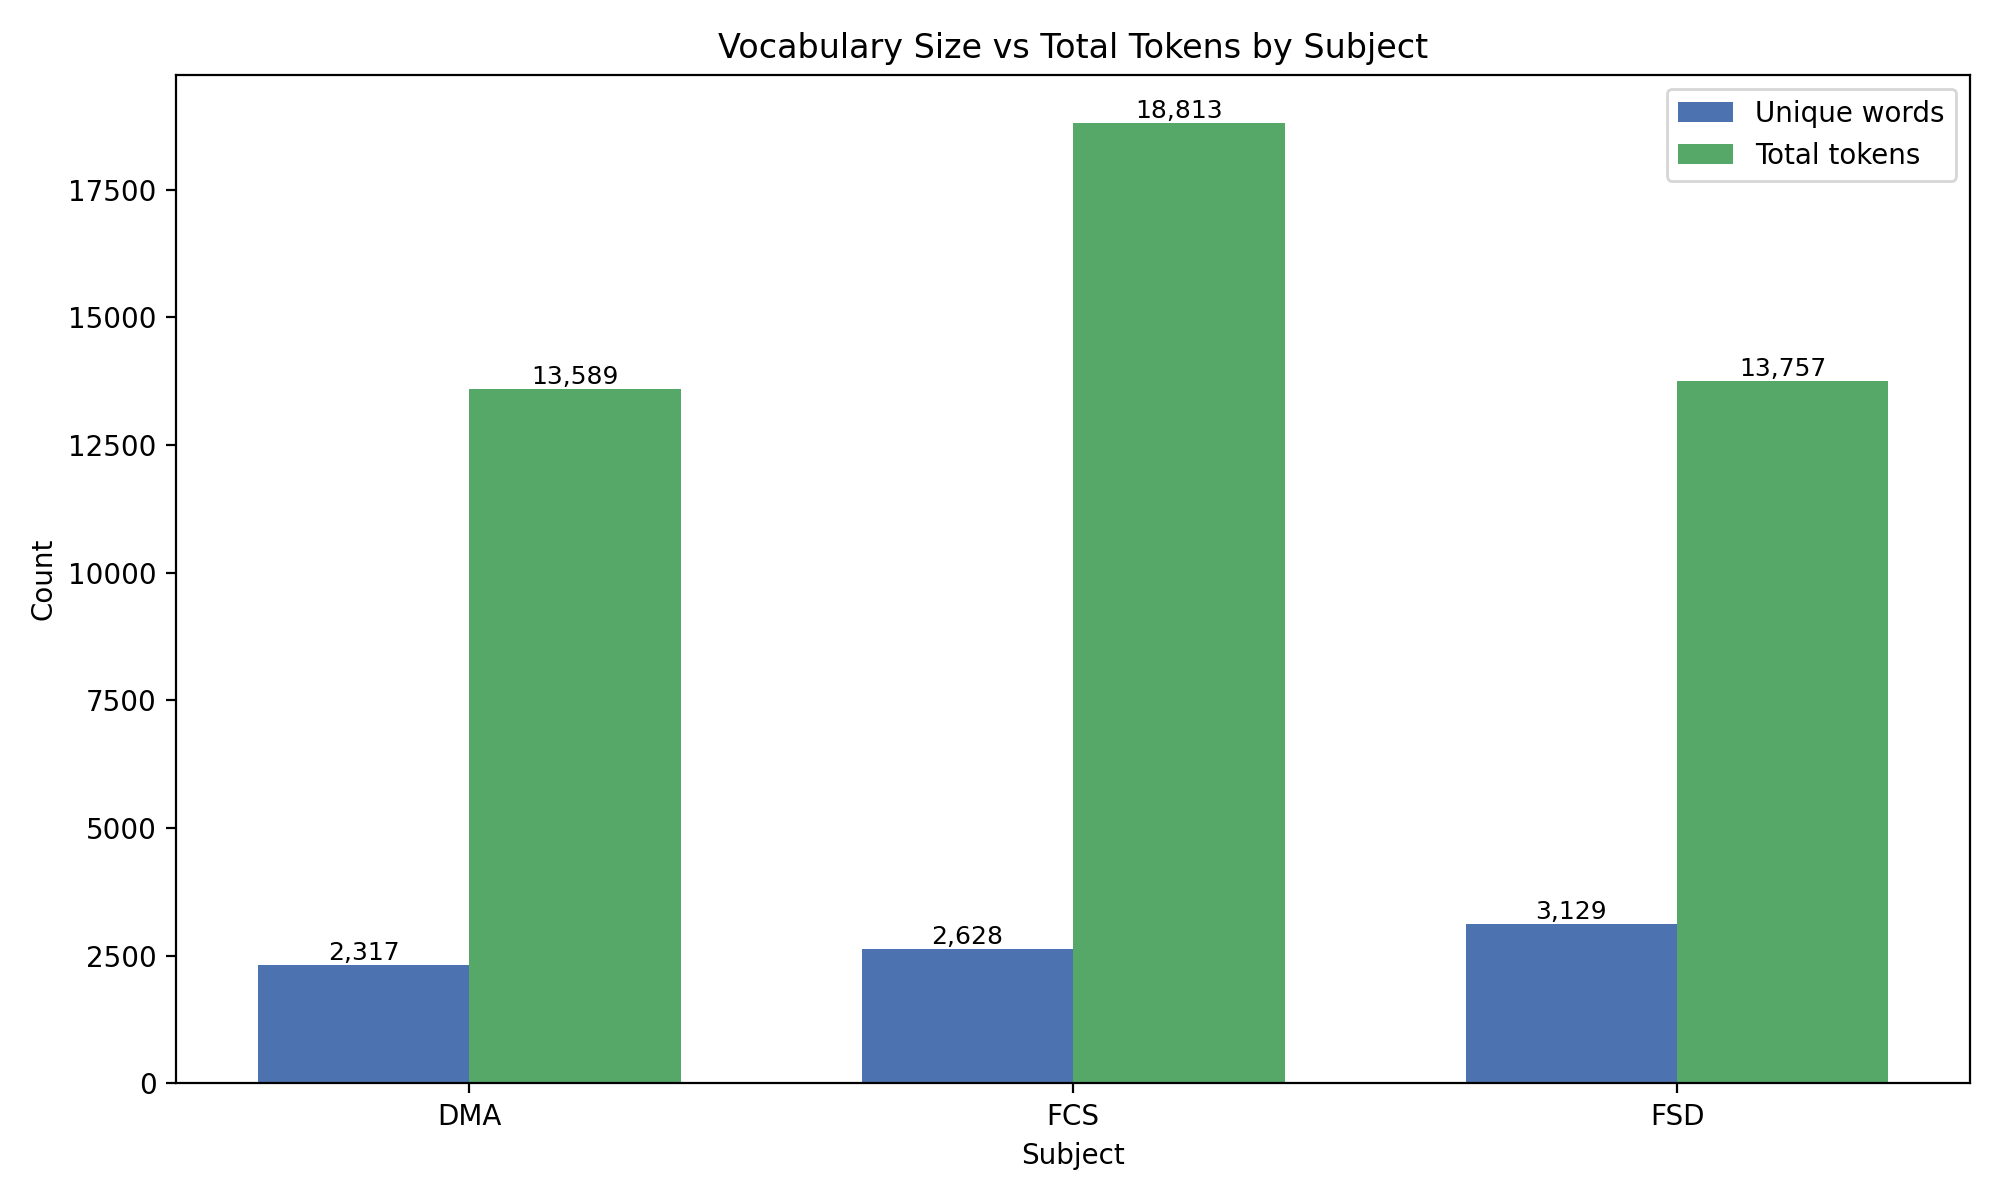
\includegraphics[width=\textwidth]{figs/vocabulary_size_comparison.png}
    \caption{Vocabulary size (unique words) versus total tokens for each subject corpus.}
    \label{fig:vocab-vs-tokens}
\end{figure}
\FloatBarrier

Figure \ref{fig:topic-stats-bubble} provides a topic-level view across all subjects. The x-axis shows total words per topic document, and bubble size represents the number of unique words, making both length outliers and lexical variation explicit.

\begin{figure}[h]
    \centering
    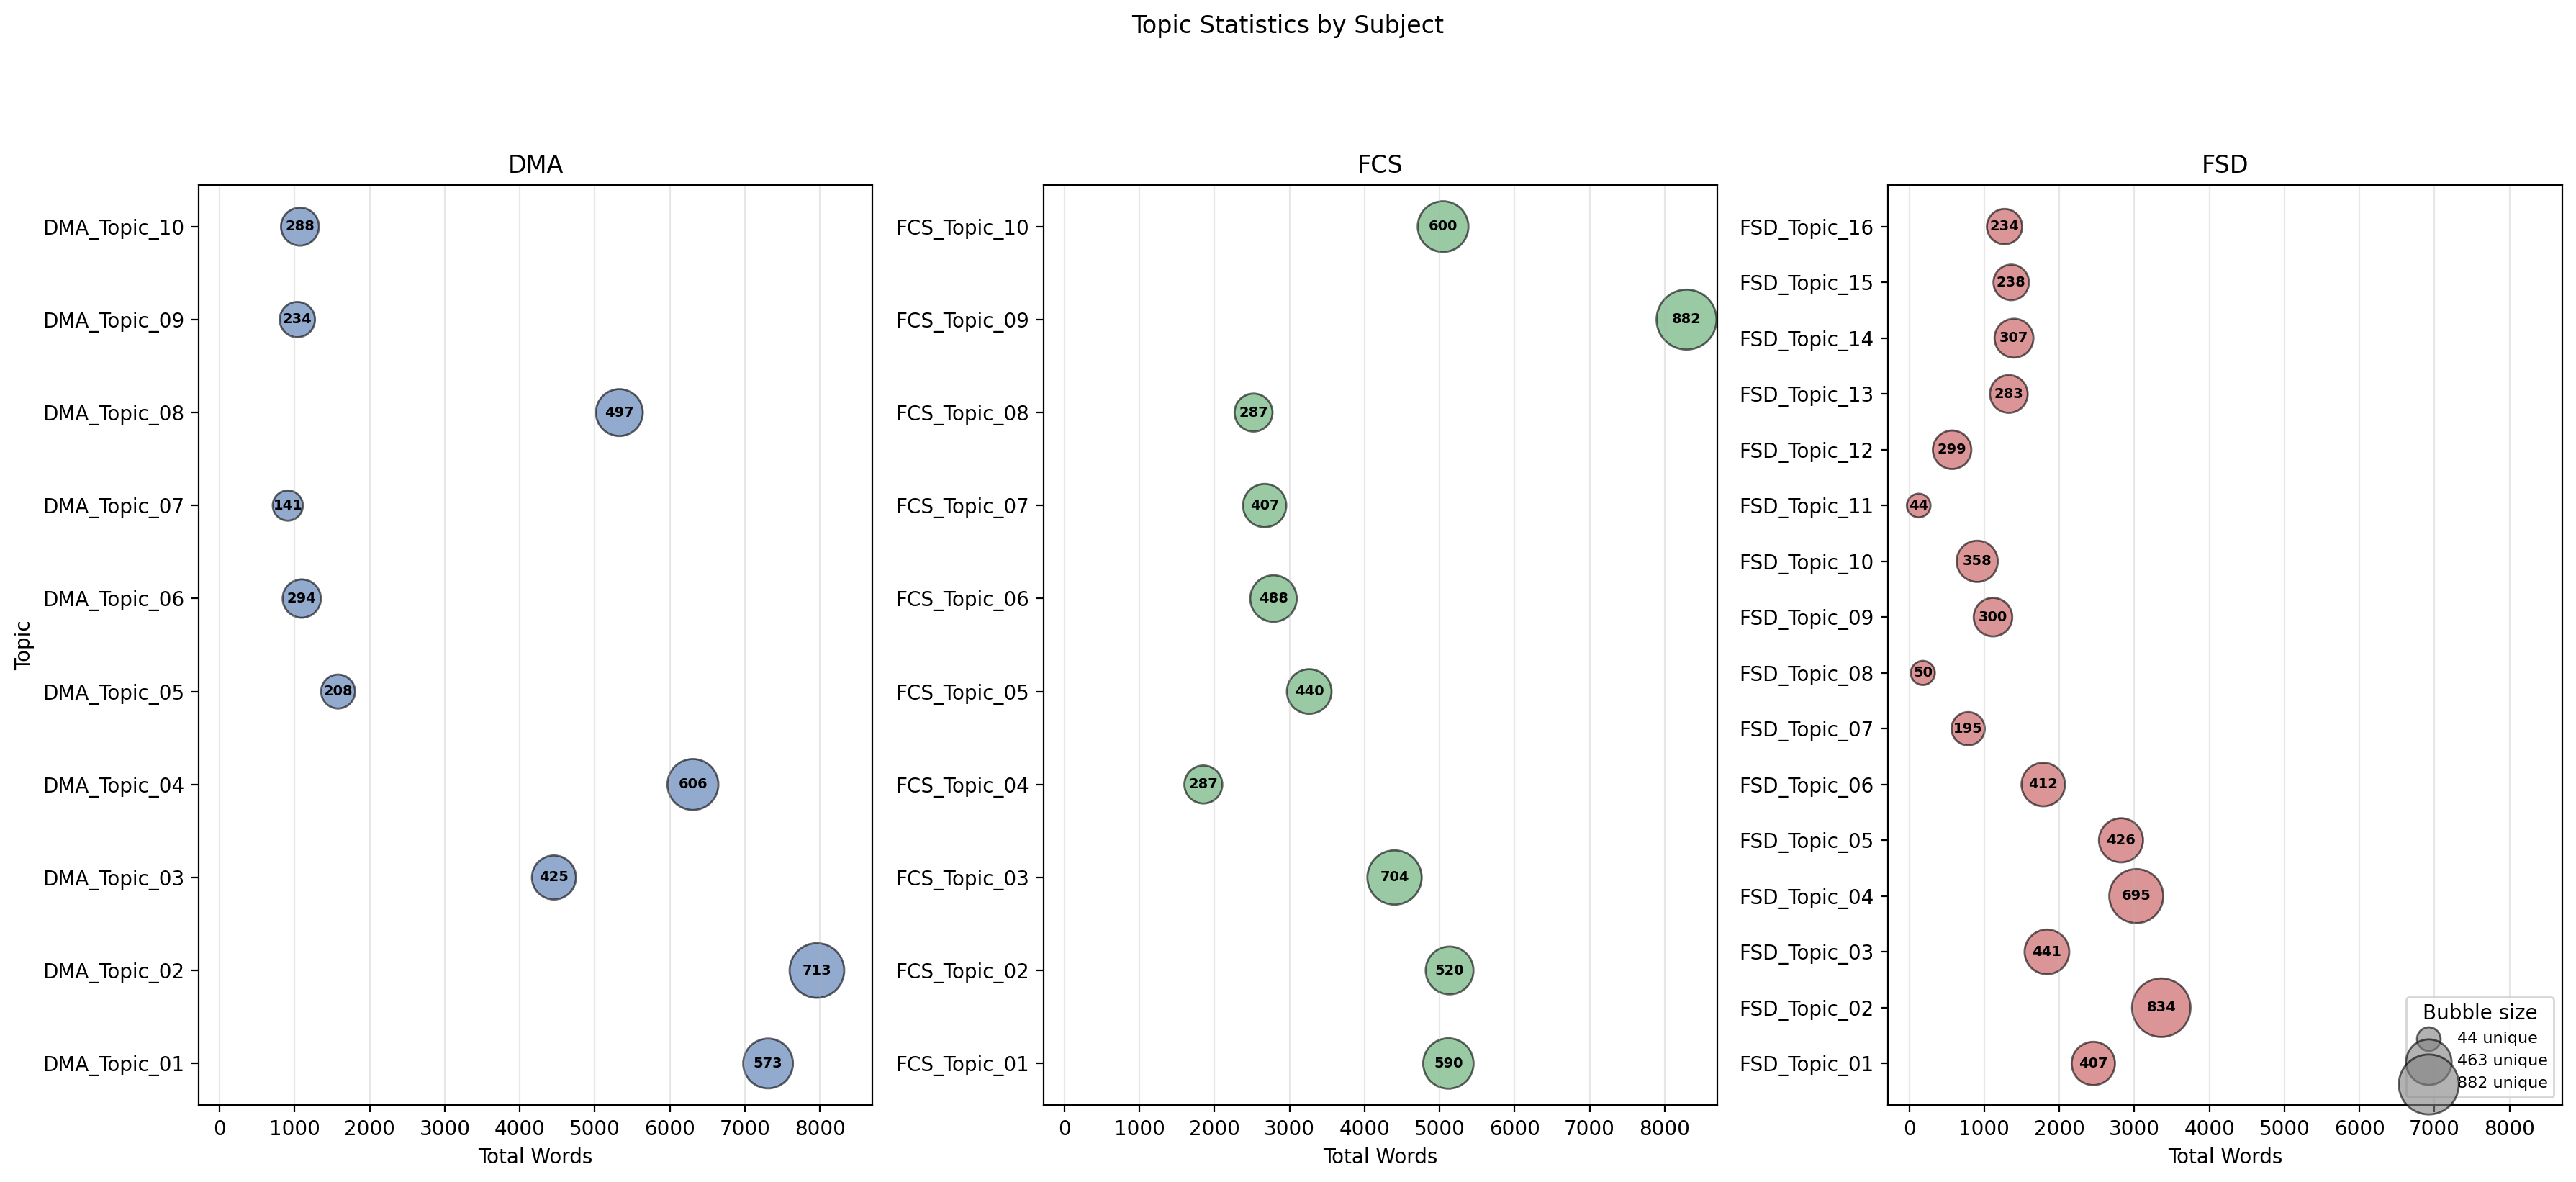
\includegraphics[width=\textwidth]{figs/all_topics_bubble.png}
    \caption{Topic-level statistics by subject. The x-axis shows total words per topic document; bubble size indicates the number of unique words.}
    \label{fig:topic-stats-bubble}
\end{figure}
\FloatBarrier

FCS contains one clear length outlier (Topic\_09 at 8,291 words), while DMA appears more polarised, combining multiple very large topics with several short ones. In FSD, most topics remain below 2,000 words, and two exceptionally short topics (126 and 181 words) stand out, consistent with limited extractable text in some slide-based materials. Bubble sizes further suggest that longer topics tend to introduce more unique terms, while FSD maintains relatively high lexical variety even in moderately sized topics.

These distributional differences motivate a unified token-based chunking strategy for downstream QA generation. Chunking is essential for long, information-dense topics (especially in FCS and DMA) to fit within the model context window, while keeping preprocessing consistent for shorter FSD topics, which typically map to a single coherent chunk.

\paragraph{Vocabulary and main topics.}
The vocabulary of each corpus was analysed using the same preprocessing pipeline. Text is converted to lowercase and URL/email patterns are removed. Tokenisation keeps only alphabetic tokens with a minimum length of two characters. Common English stop words and a small set of domain-specific stop words are removed. Finally, the remaining tokens are lemmatised.

Based on these tokens, a word cloud and a bar chart of the 20 most frequent content words were generated for each module (Figures \ref{fig:fsd-wordcloud}-\ref{fig:dma-topwords}). In addition, frequent bigrams and trigrams were computed to highlight repeated multi-word phrases in the materials (Figures \ref{fig:fsd-bigrams}-\ref{fig:dma-trigrams}).

For FSD, frequent content words include statement, printf, loop, program, variable, value and function. Frequent bigrams and trigrams like "include stdio", "stdio int main", and "task write program" show repeated code patterns and repeated task instructions. Overall, the results confirm that the FSD materials focus on basic programming syntax, control flow and code examples.

\begin{figure}[h]
    \centering
    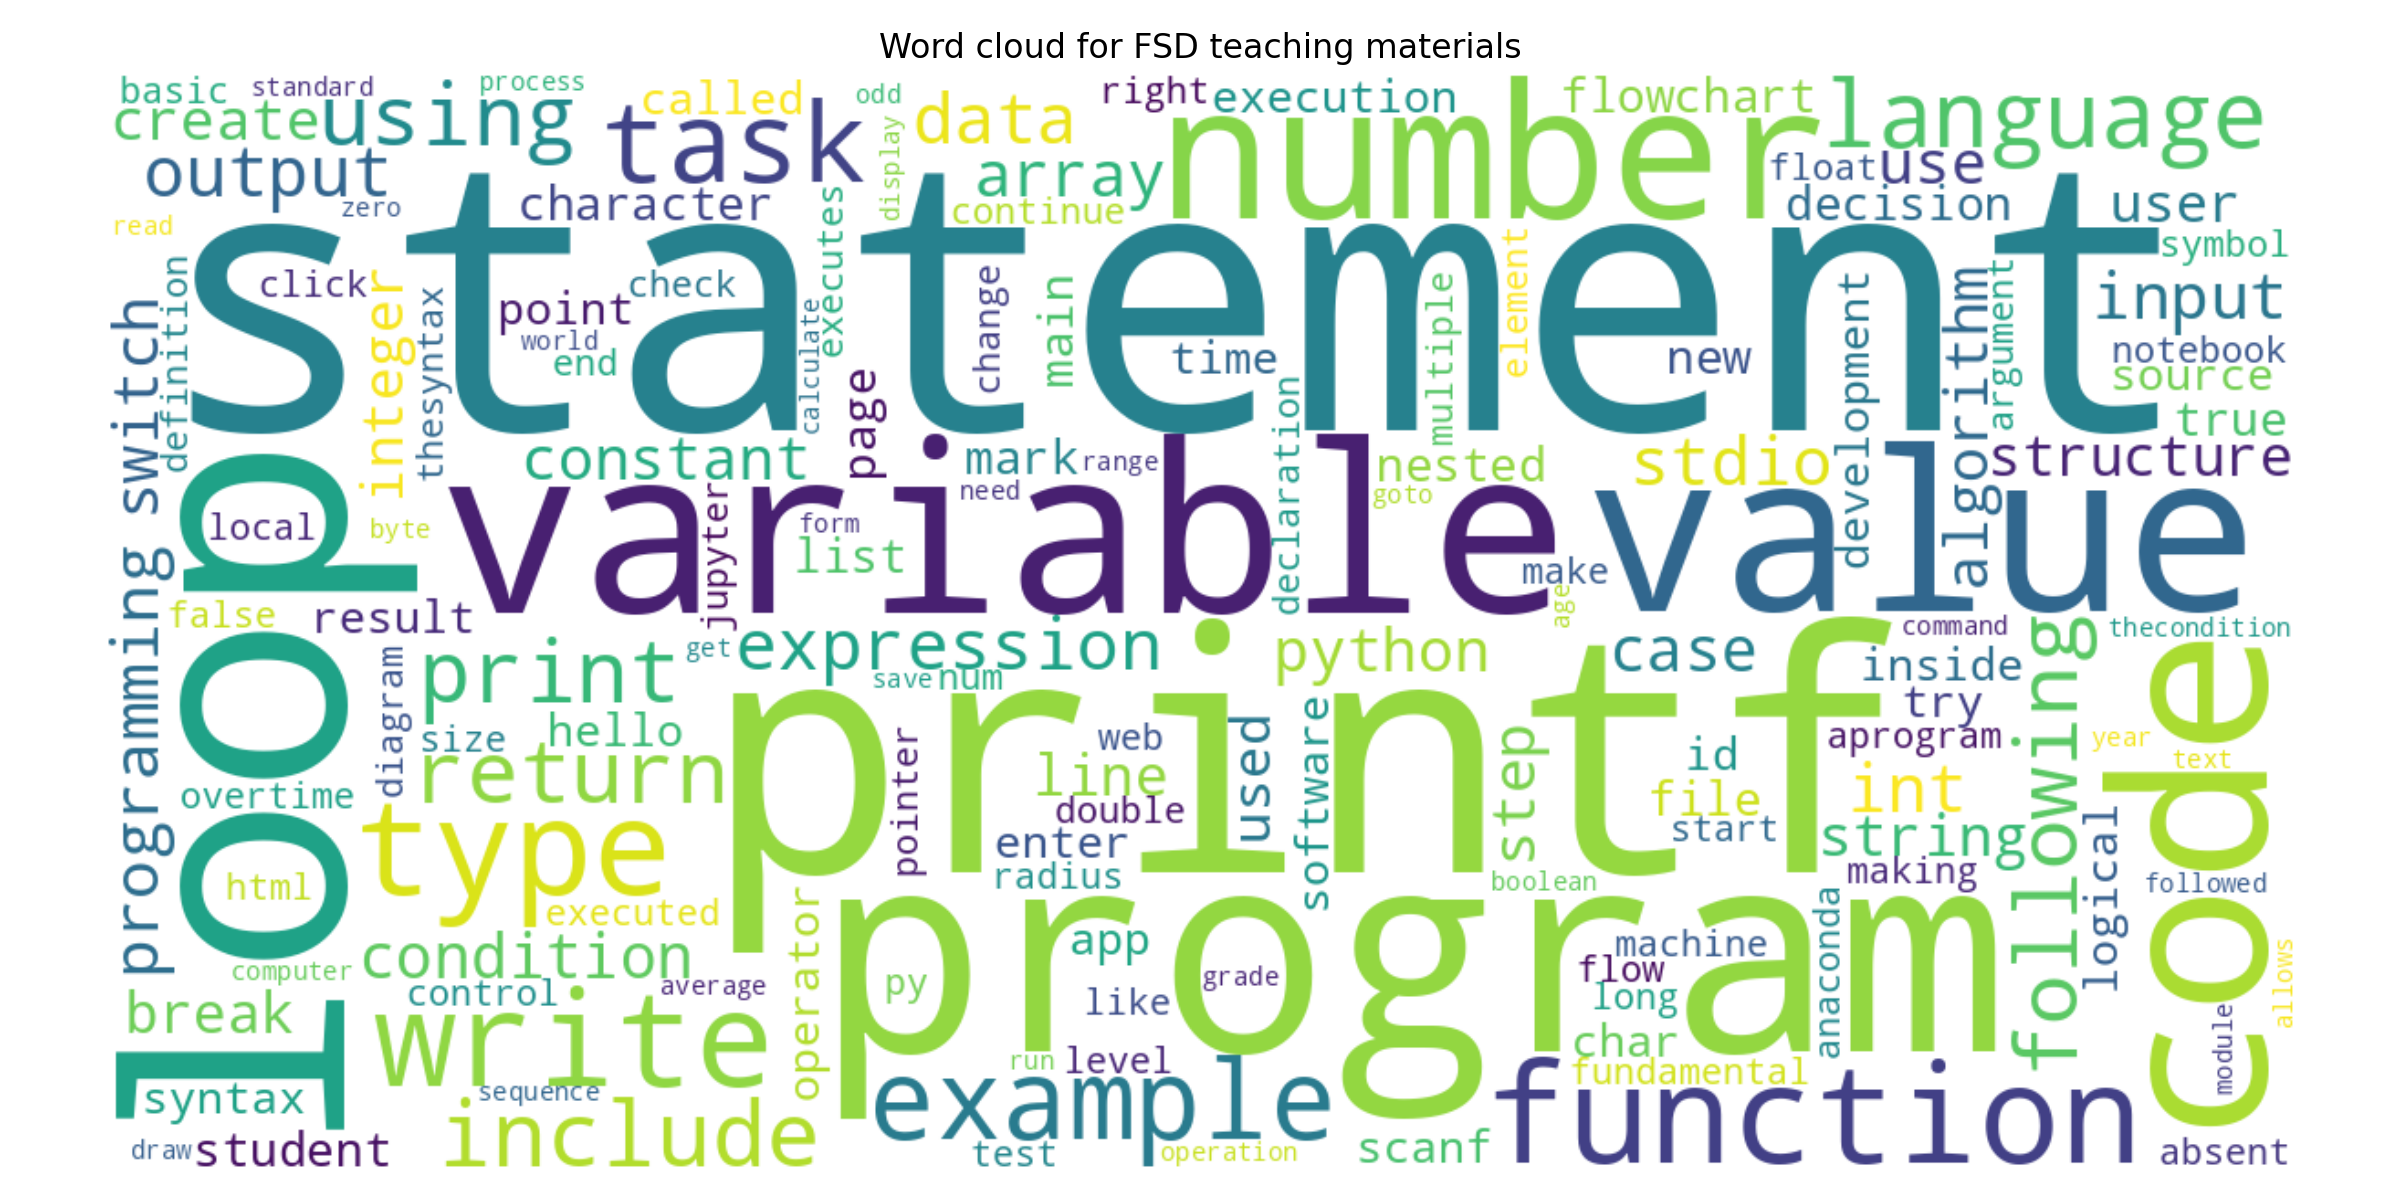
\includegraphics[width=\textwidth]{figs/FSD_wordcloud.png}
    \caption{Word cloud for the top content words in the FSD teaching materials.}
    \label{fig:fsd-wordcloud}
\end{figure}
\FloatBarrier

\begin{figure}[h]
    \centering
    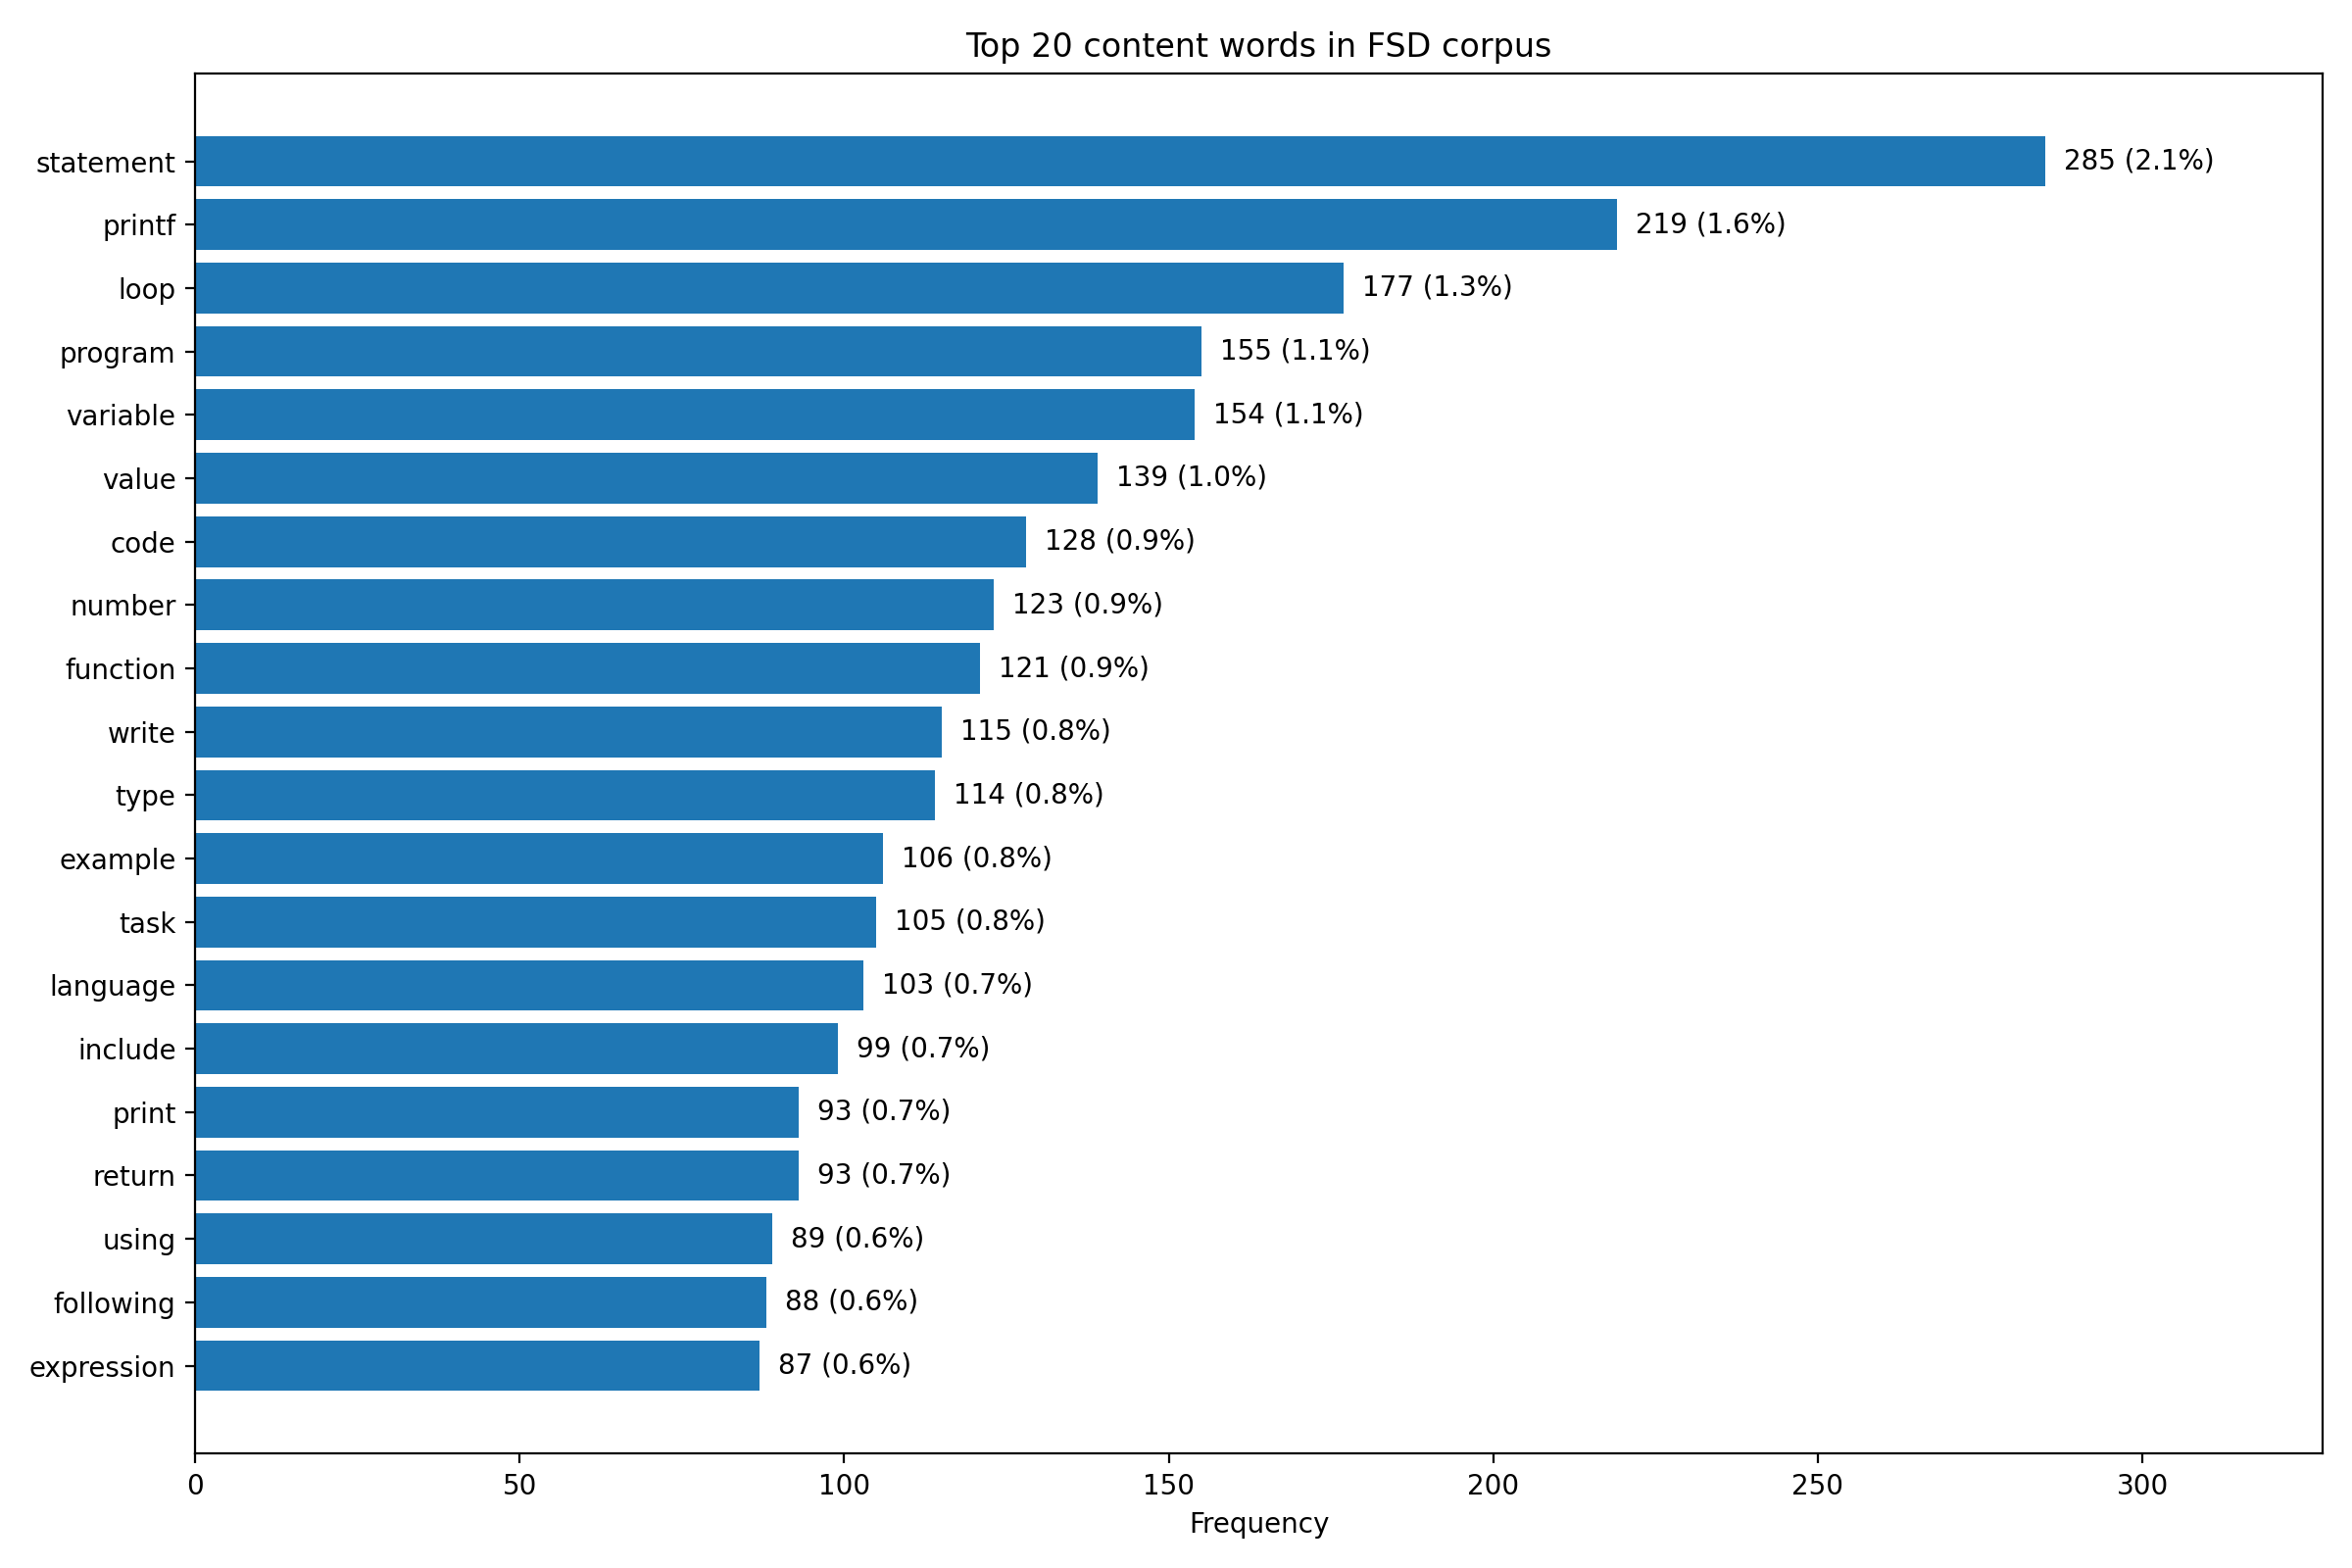
\includegraphics[width=\textwidth]{figs/FSD_top_words.png}
    \caption{Top 20 content words in the FSD corpus with their frequencies.}
    \label{fig:fsd-topwords}
\end{figure}
\FloatBarrier

\begin{figure}[h]
    \centering
    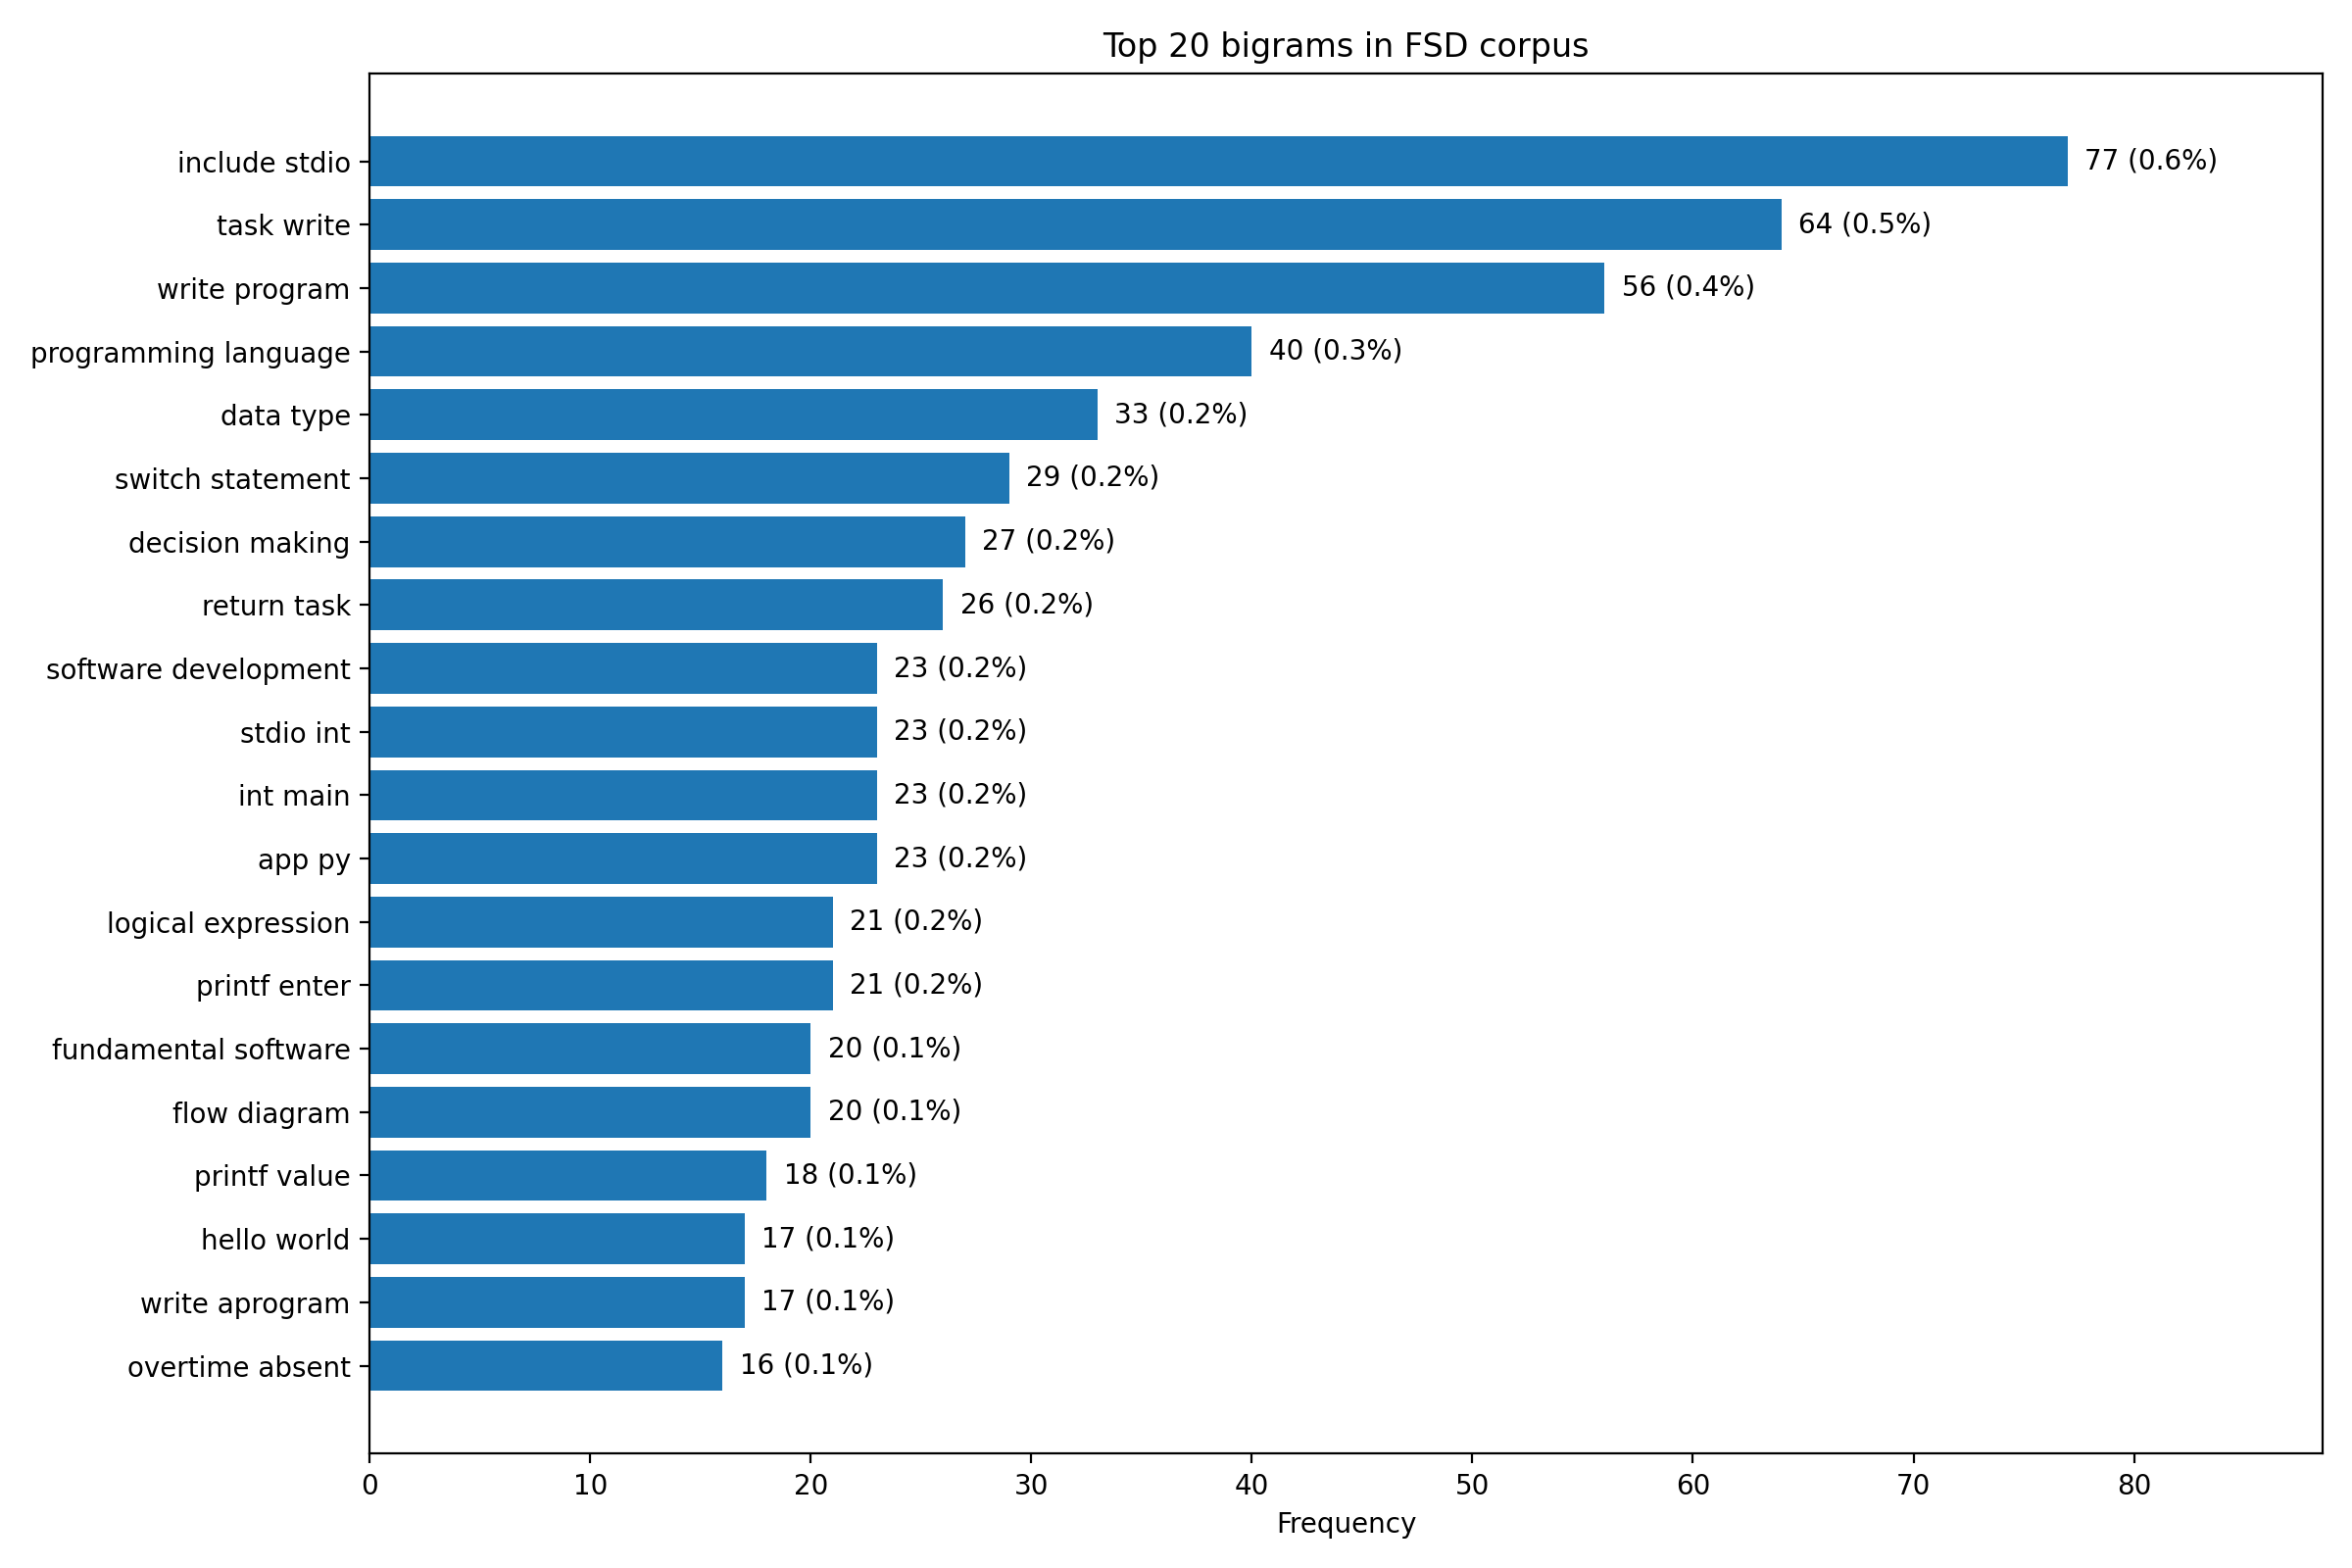
\includegraphics[width=\textwidth]{figs/FSD_top_bigrams.png}
    \caption{Top 20 bigrams in the FSD corpus.}
    \label{fig:fsd-bigrams}
\end{figure}
\FloatBarrier

\begin{figure}[h]
    \centering
    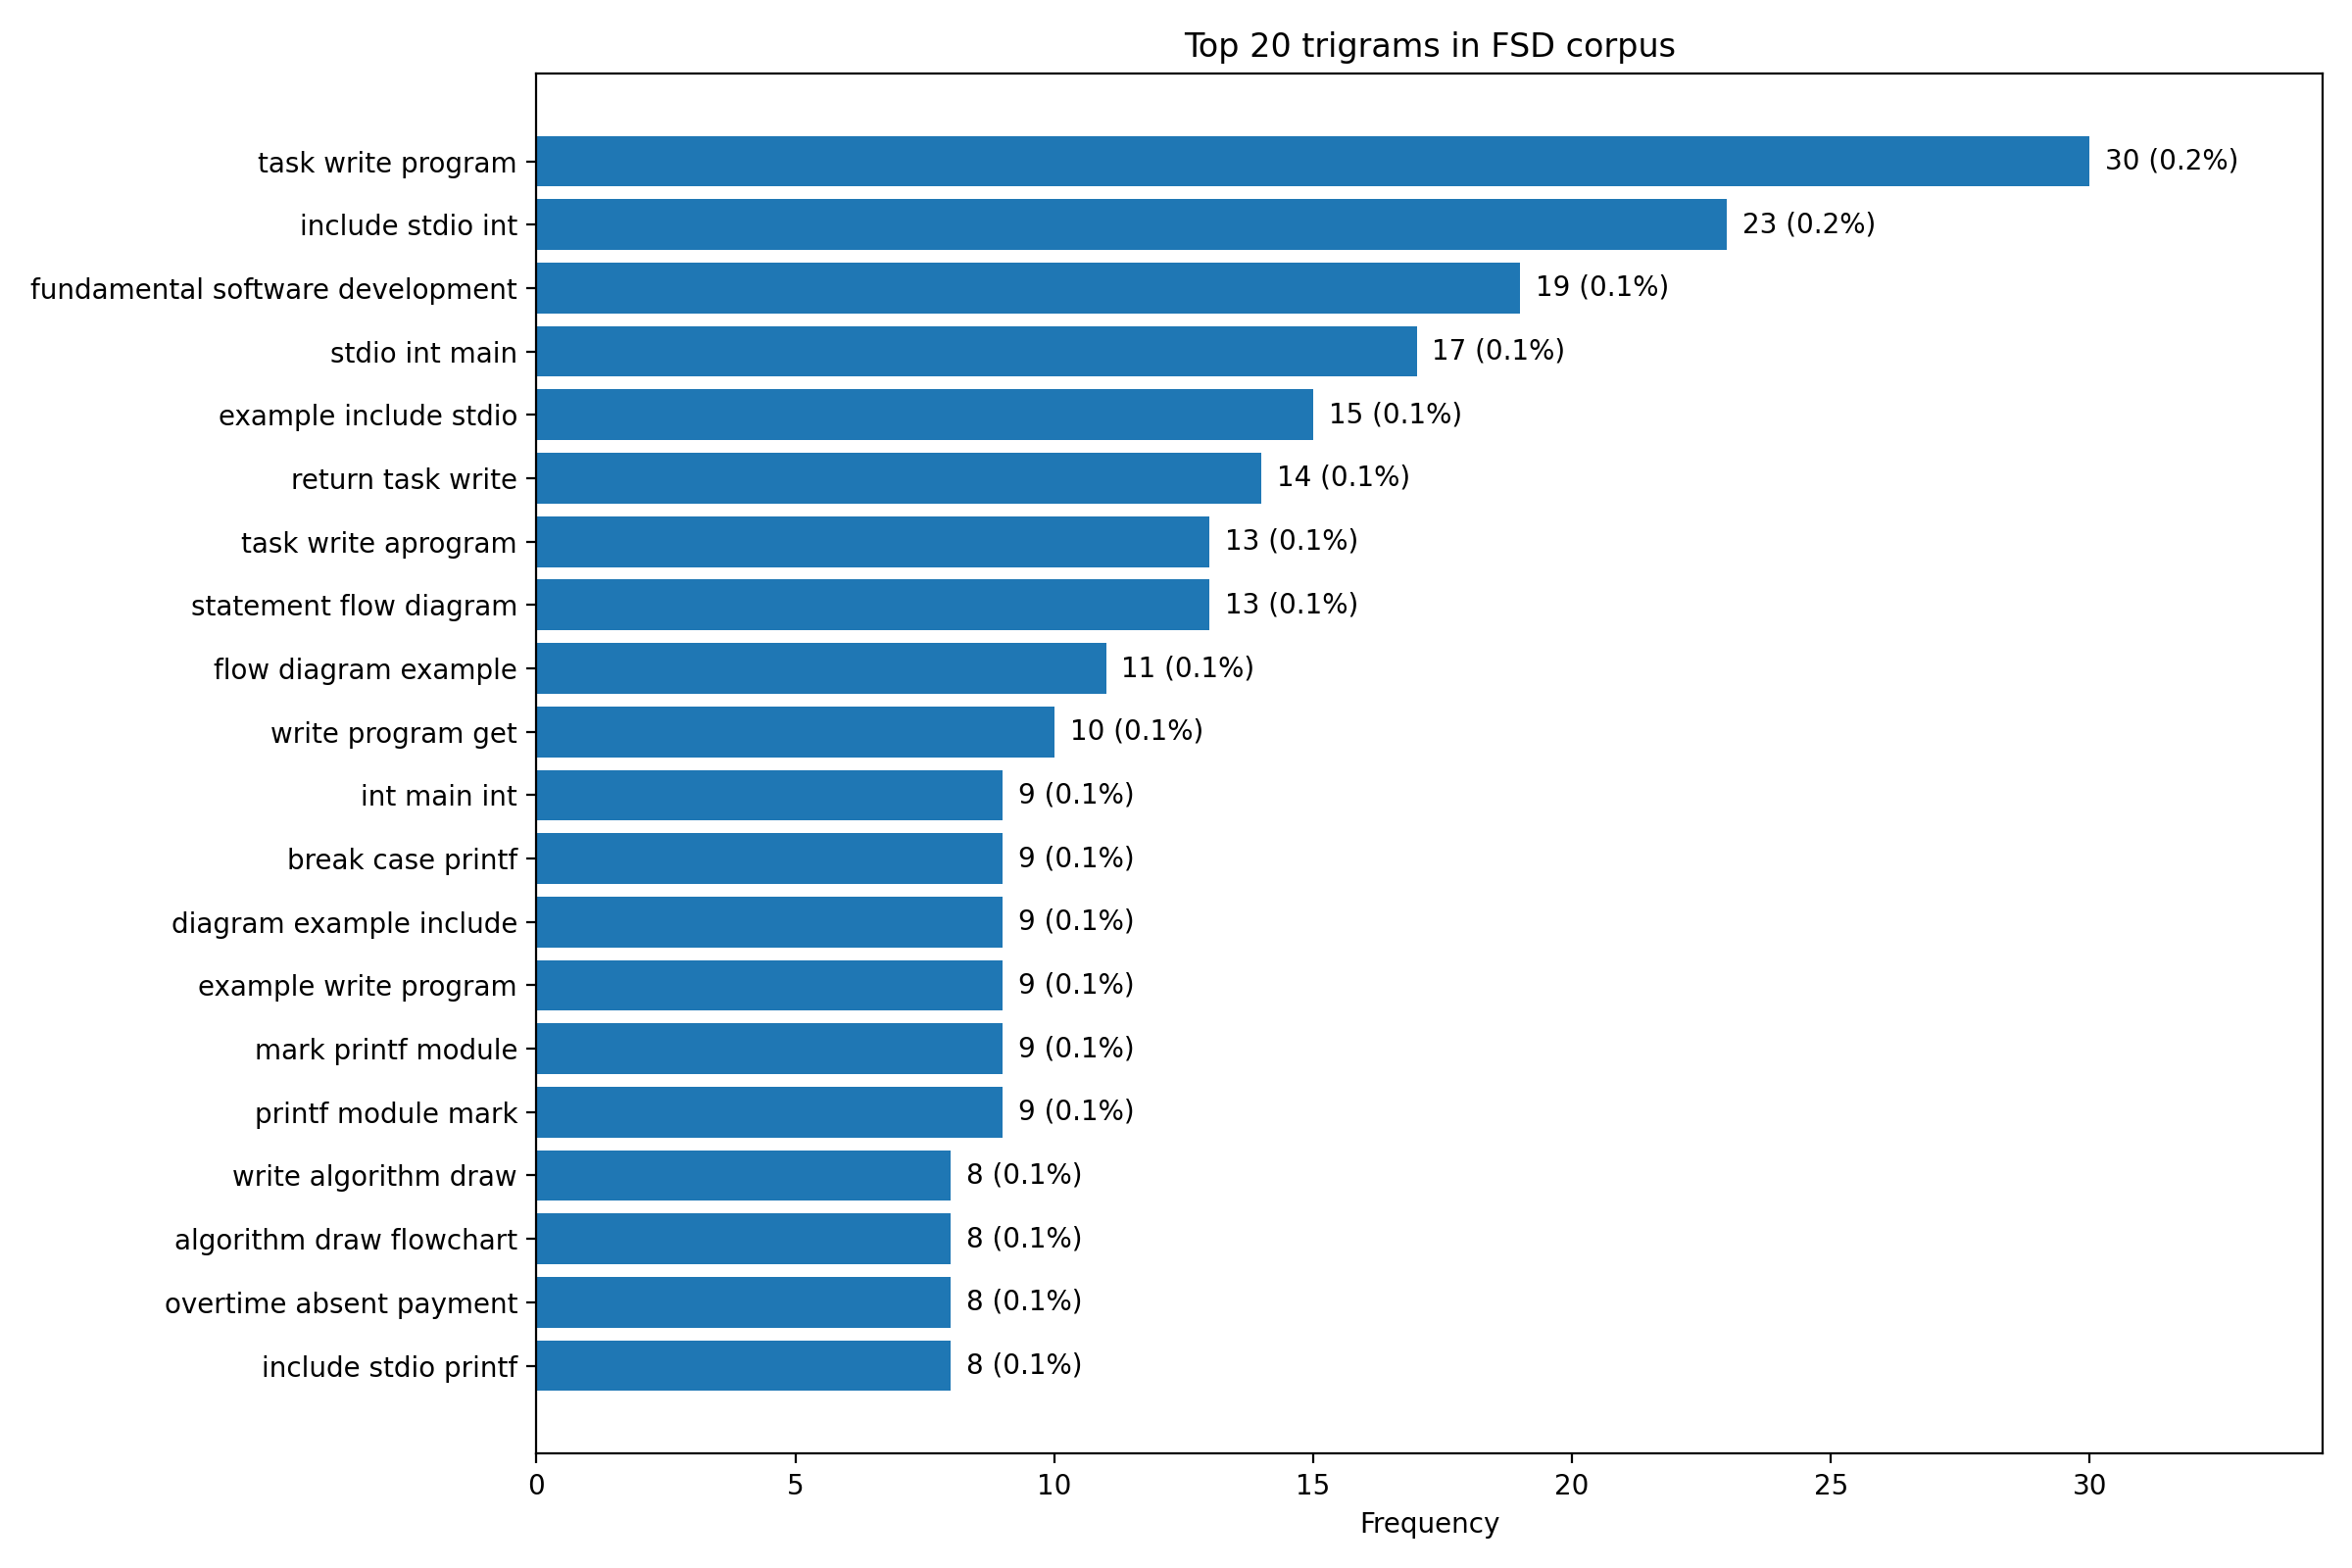
\includegraphics[width=\textwidth]{figs/FSD_top_trigrams.png}
    \caption{Top 20 trigrams in the FSD corpus.}
    \label{fig:fsd-trigrams}
\end{figure}
\FloatBarrier

For FCS, the top content words such as data, bit, number, memory, cpu, binary and instruction reflect the focus on data representation and computer architecture. At the n-gram level, the results contain both meaningful technical phrases like "binary number" and "memory location" and repeated institutional headers like "csi fcs". This suggests that removing headers and footers could further improve the quality of the text.

\begin{figure}[h]
    \centering
    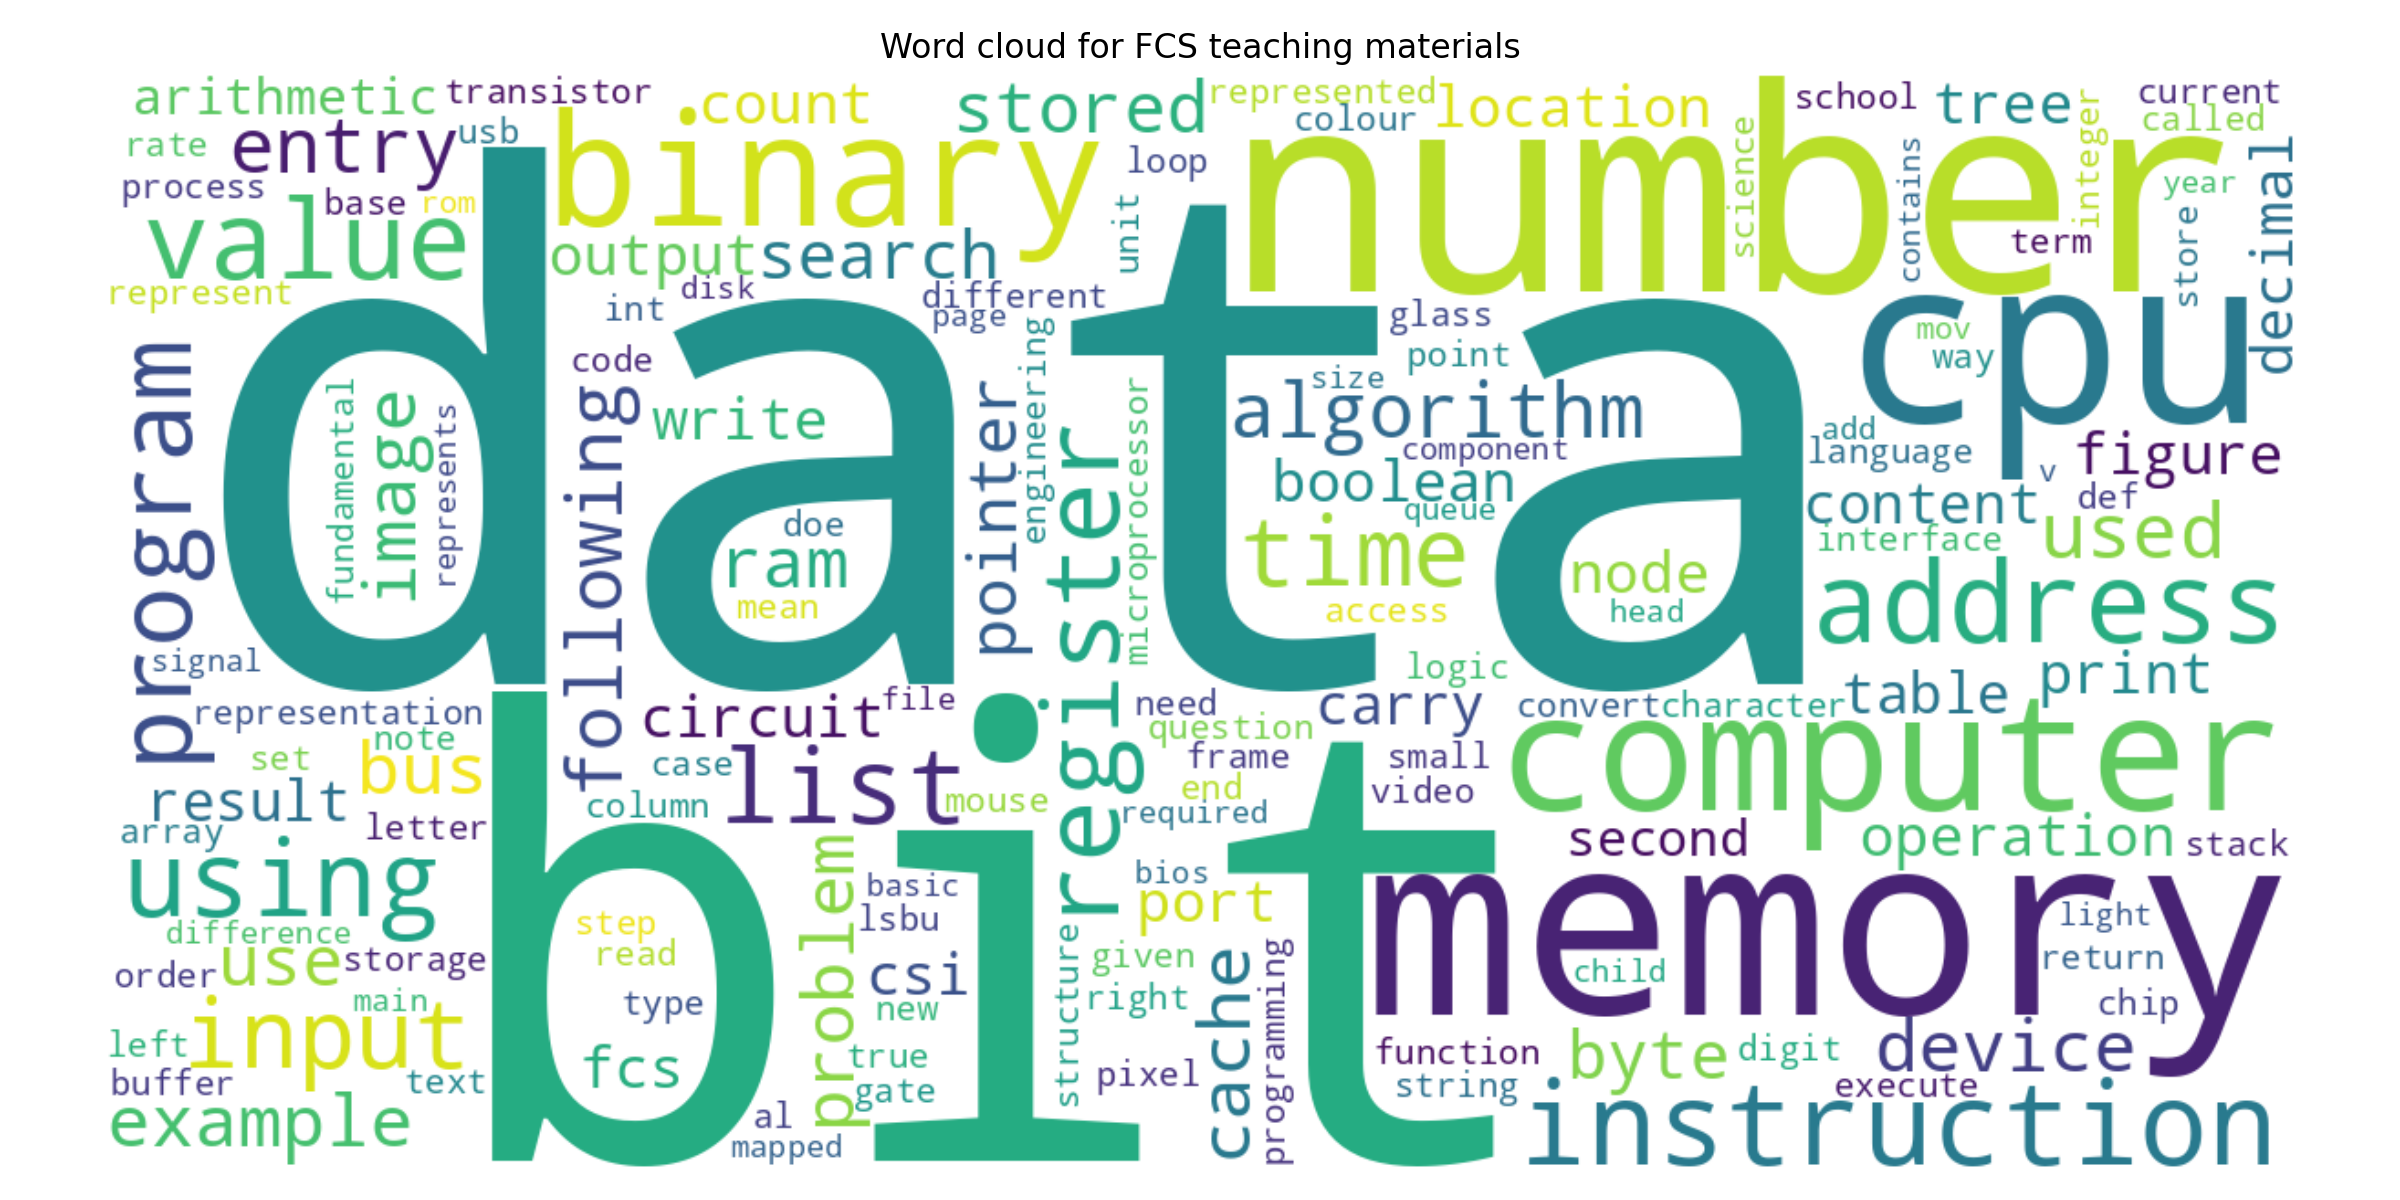
\includegraphics[width=\textwidth]{figs/FCS_wordcloud.png}
    \caption{Word cloud for the top content words in the FCS teaching materials.}
    \label{fig:fcs-wordcloud}
\end{figure}
\FloatBarrier

\begin{figure}[h]
    \centering
    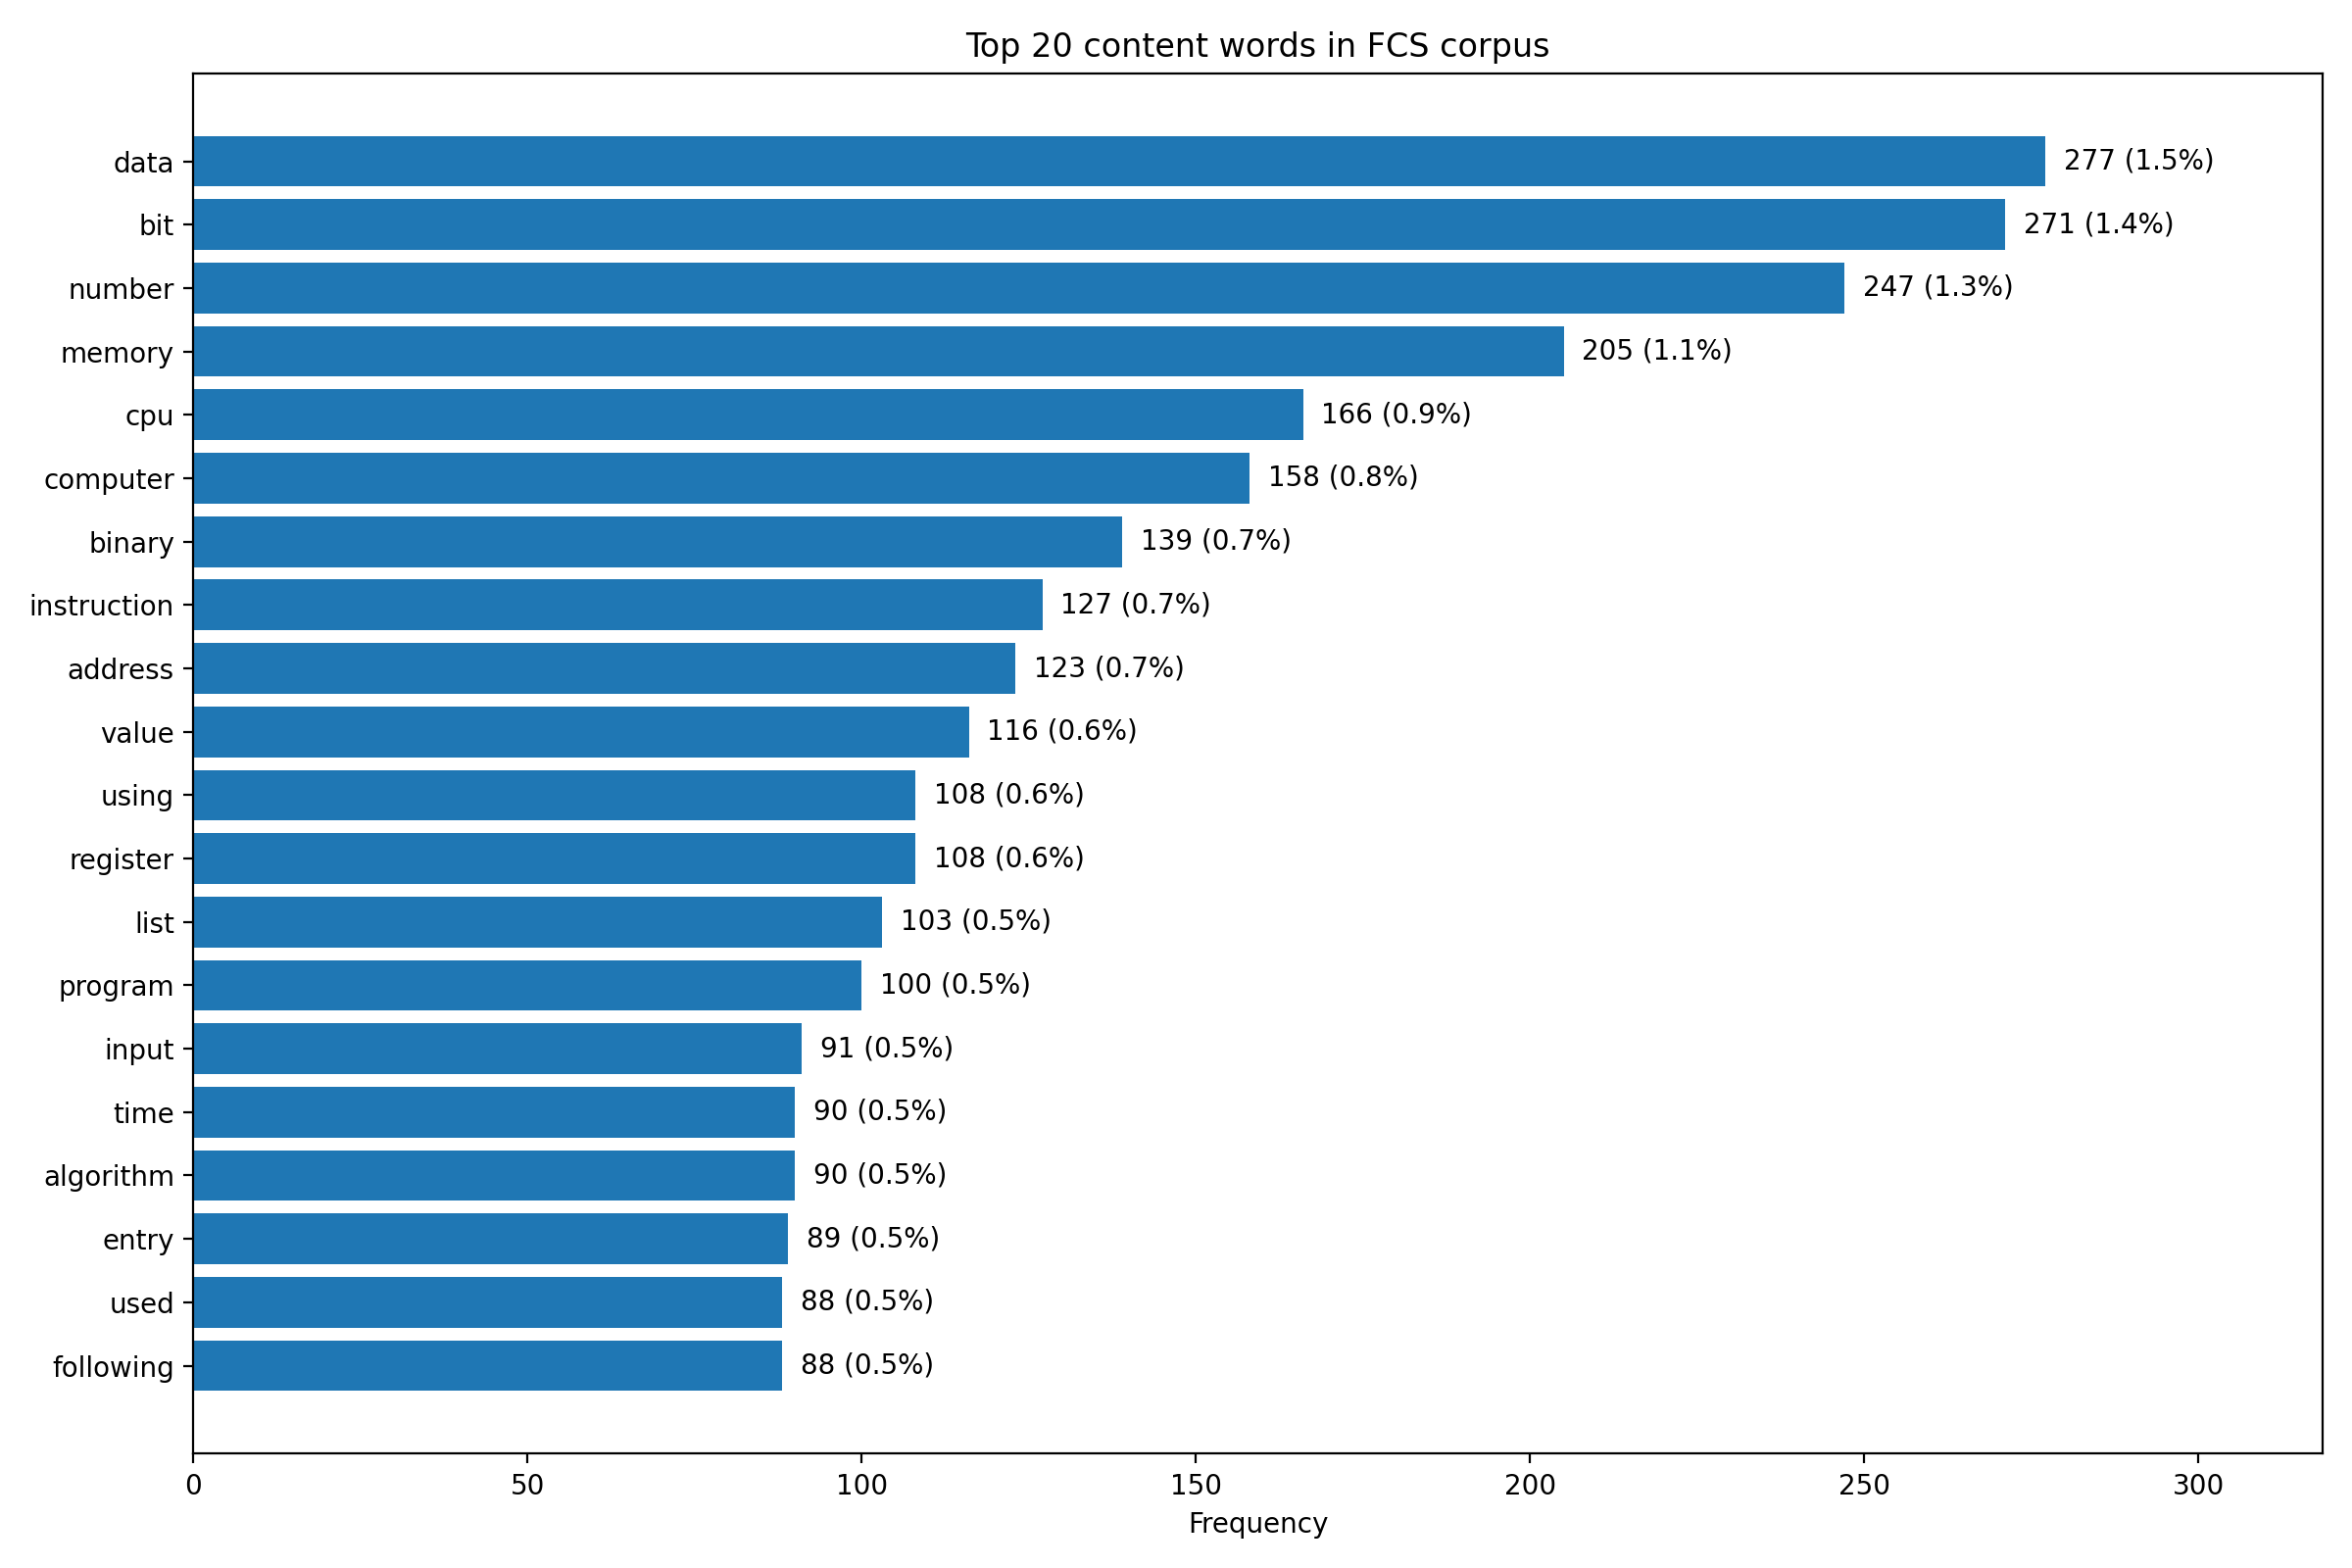
\includegraphics[width=\textwidth]{figs/FCS_top_words.png}
    \caption{Top 20 content words in the FCS corpus with their frequencies.}
    \label{fig:fcs-topwords}
\end{figure}
\FloatBarrier

\begin{figure}[h]
    \centering
    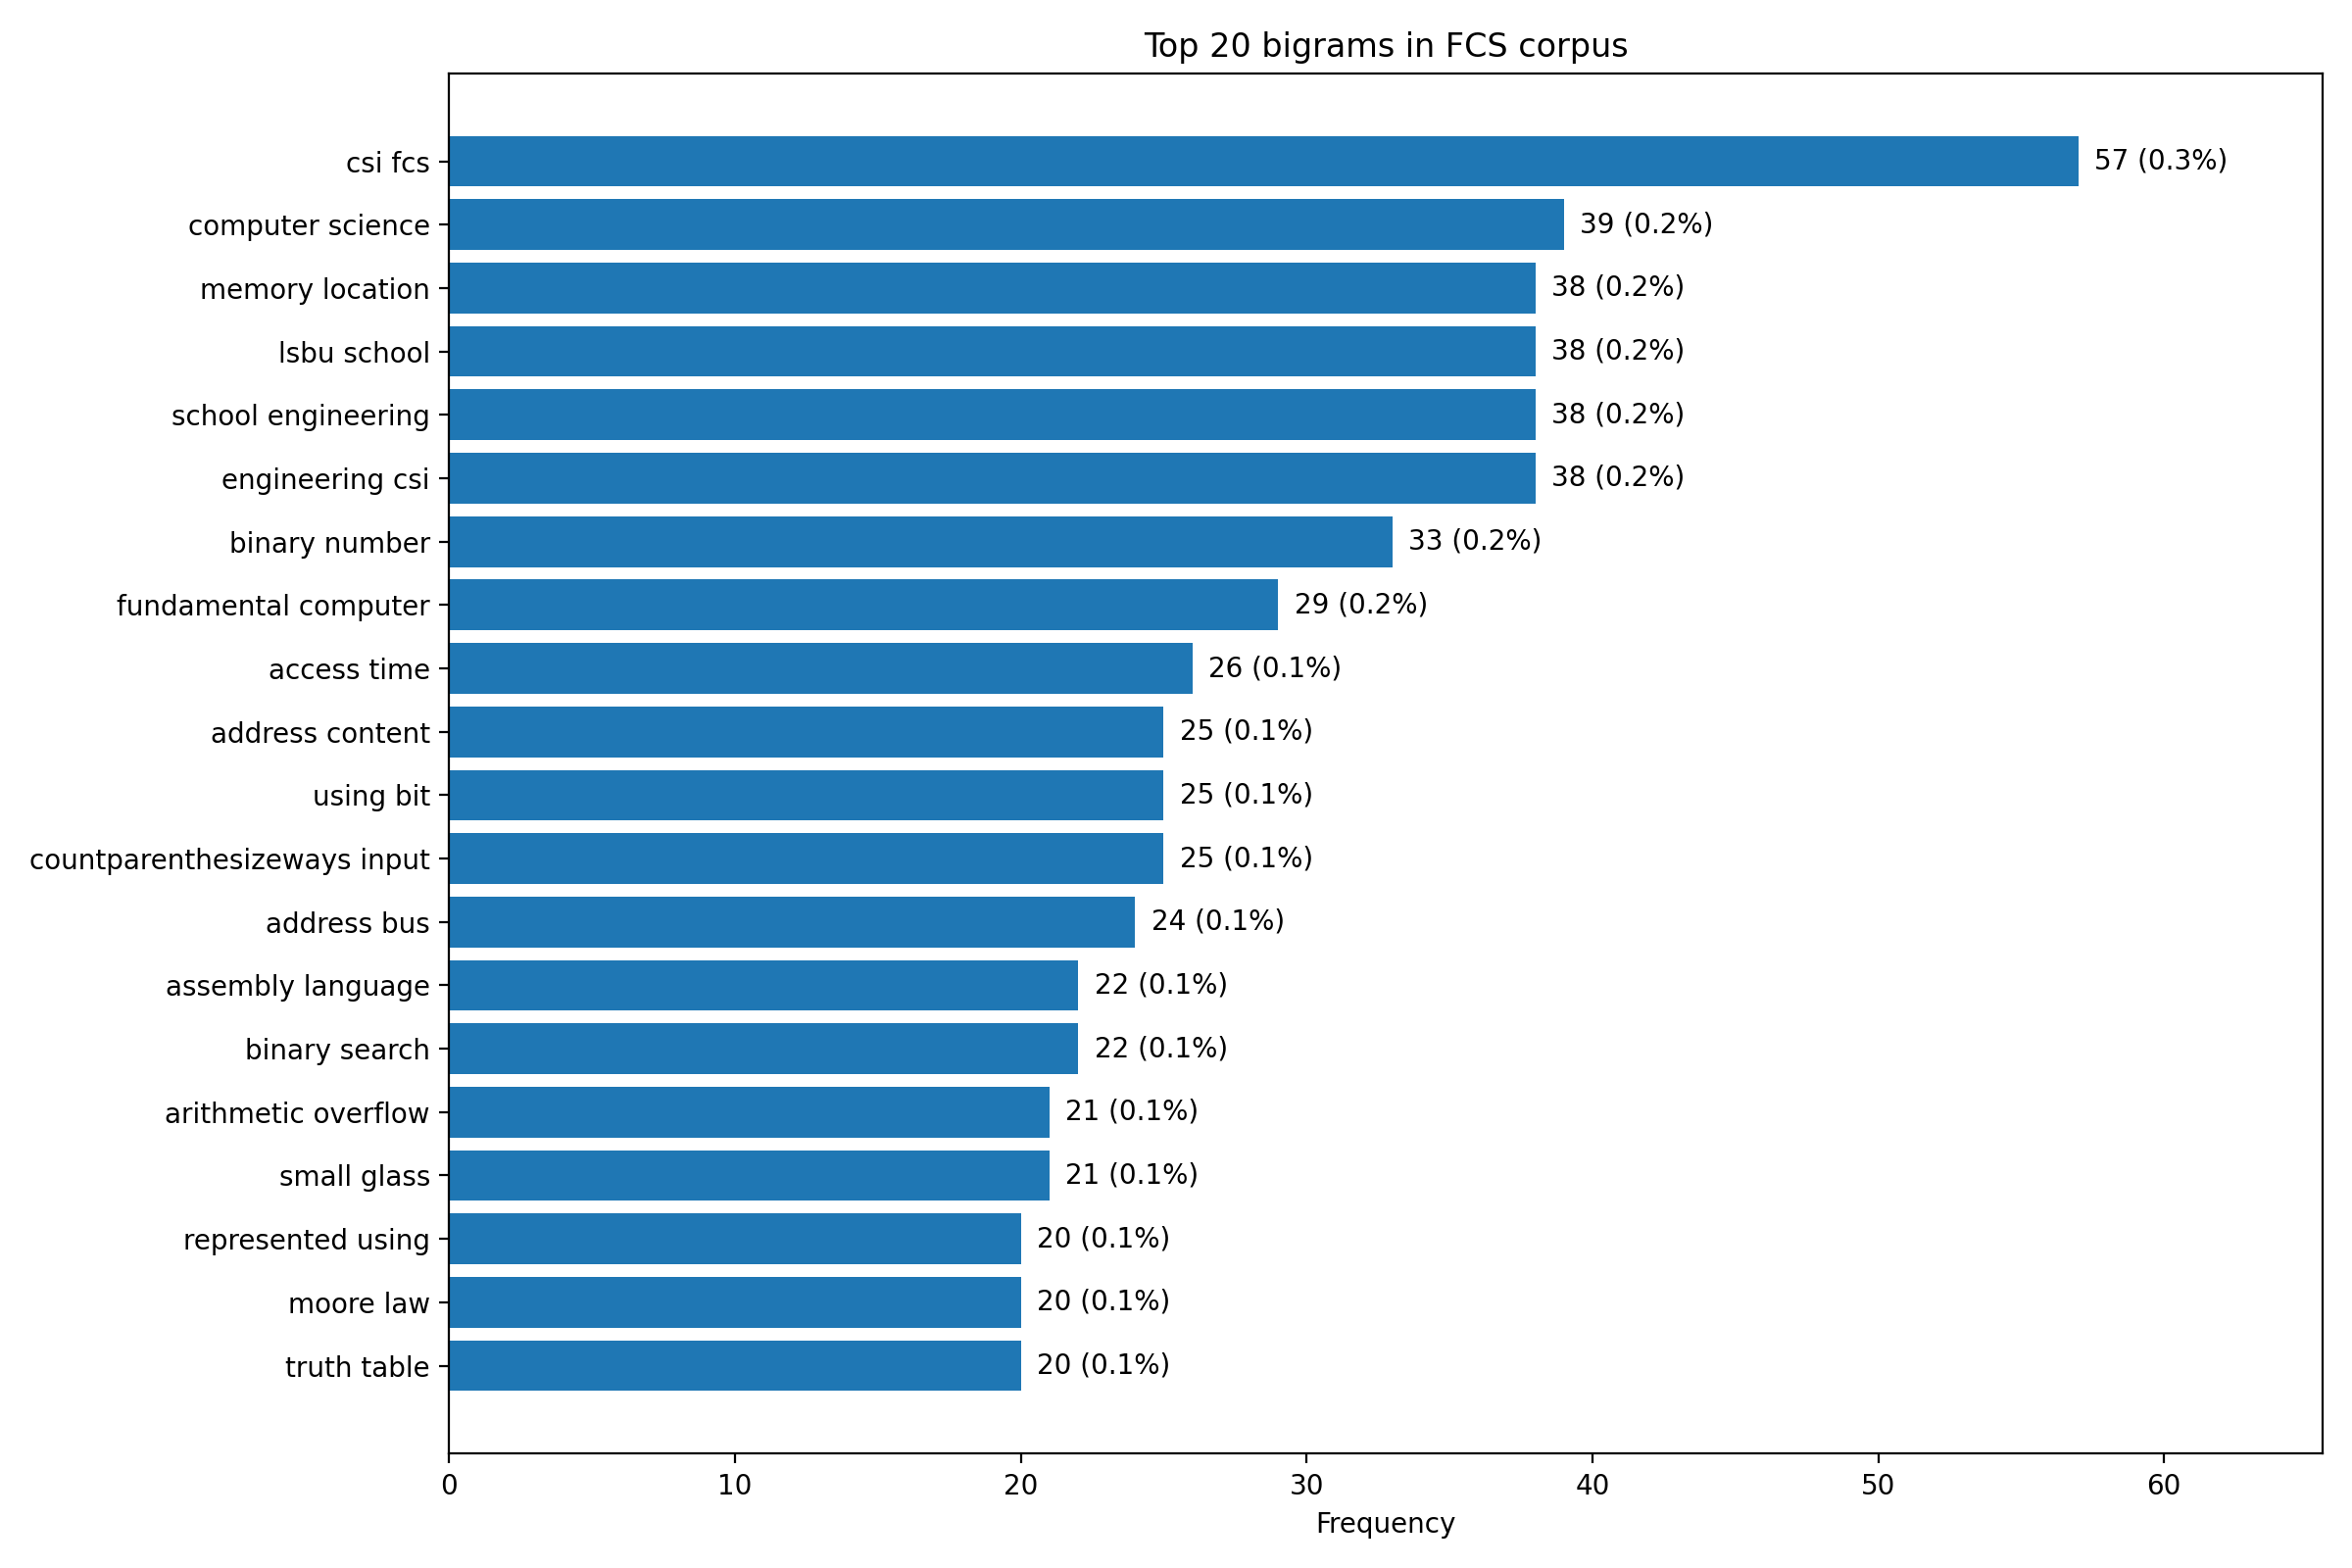
\includegraphics[width=\textwidth]{figs/FCS_top_bigrams.png}
    \caption{Top 20 bigrams in the FCS corpus.}
    \label{fig:fcs-bigrams}
\end{figure}
\FloatBarrier

\begin{figure}[h]
    \centering
    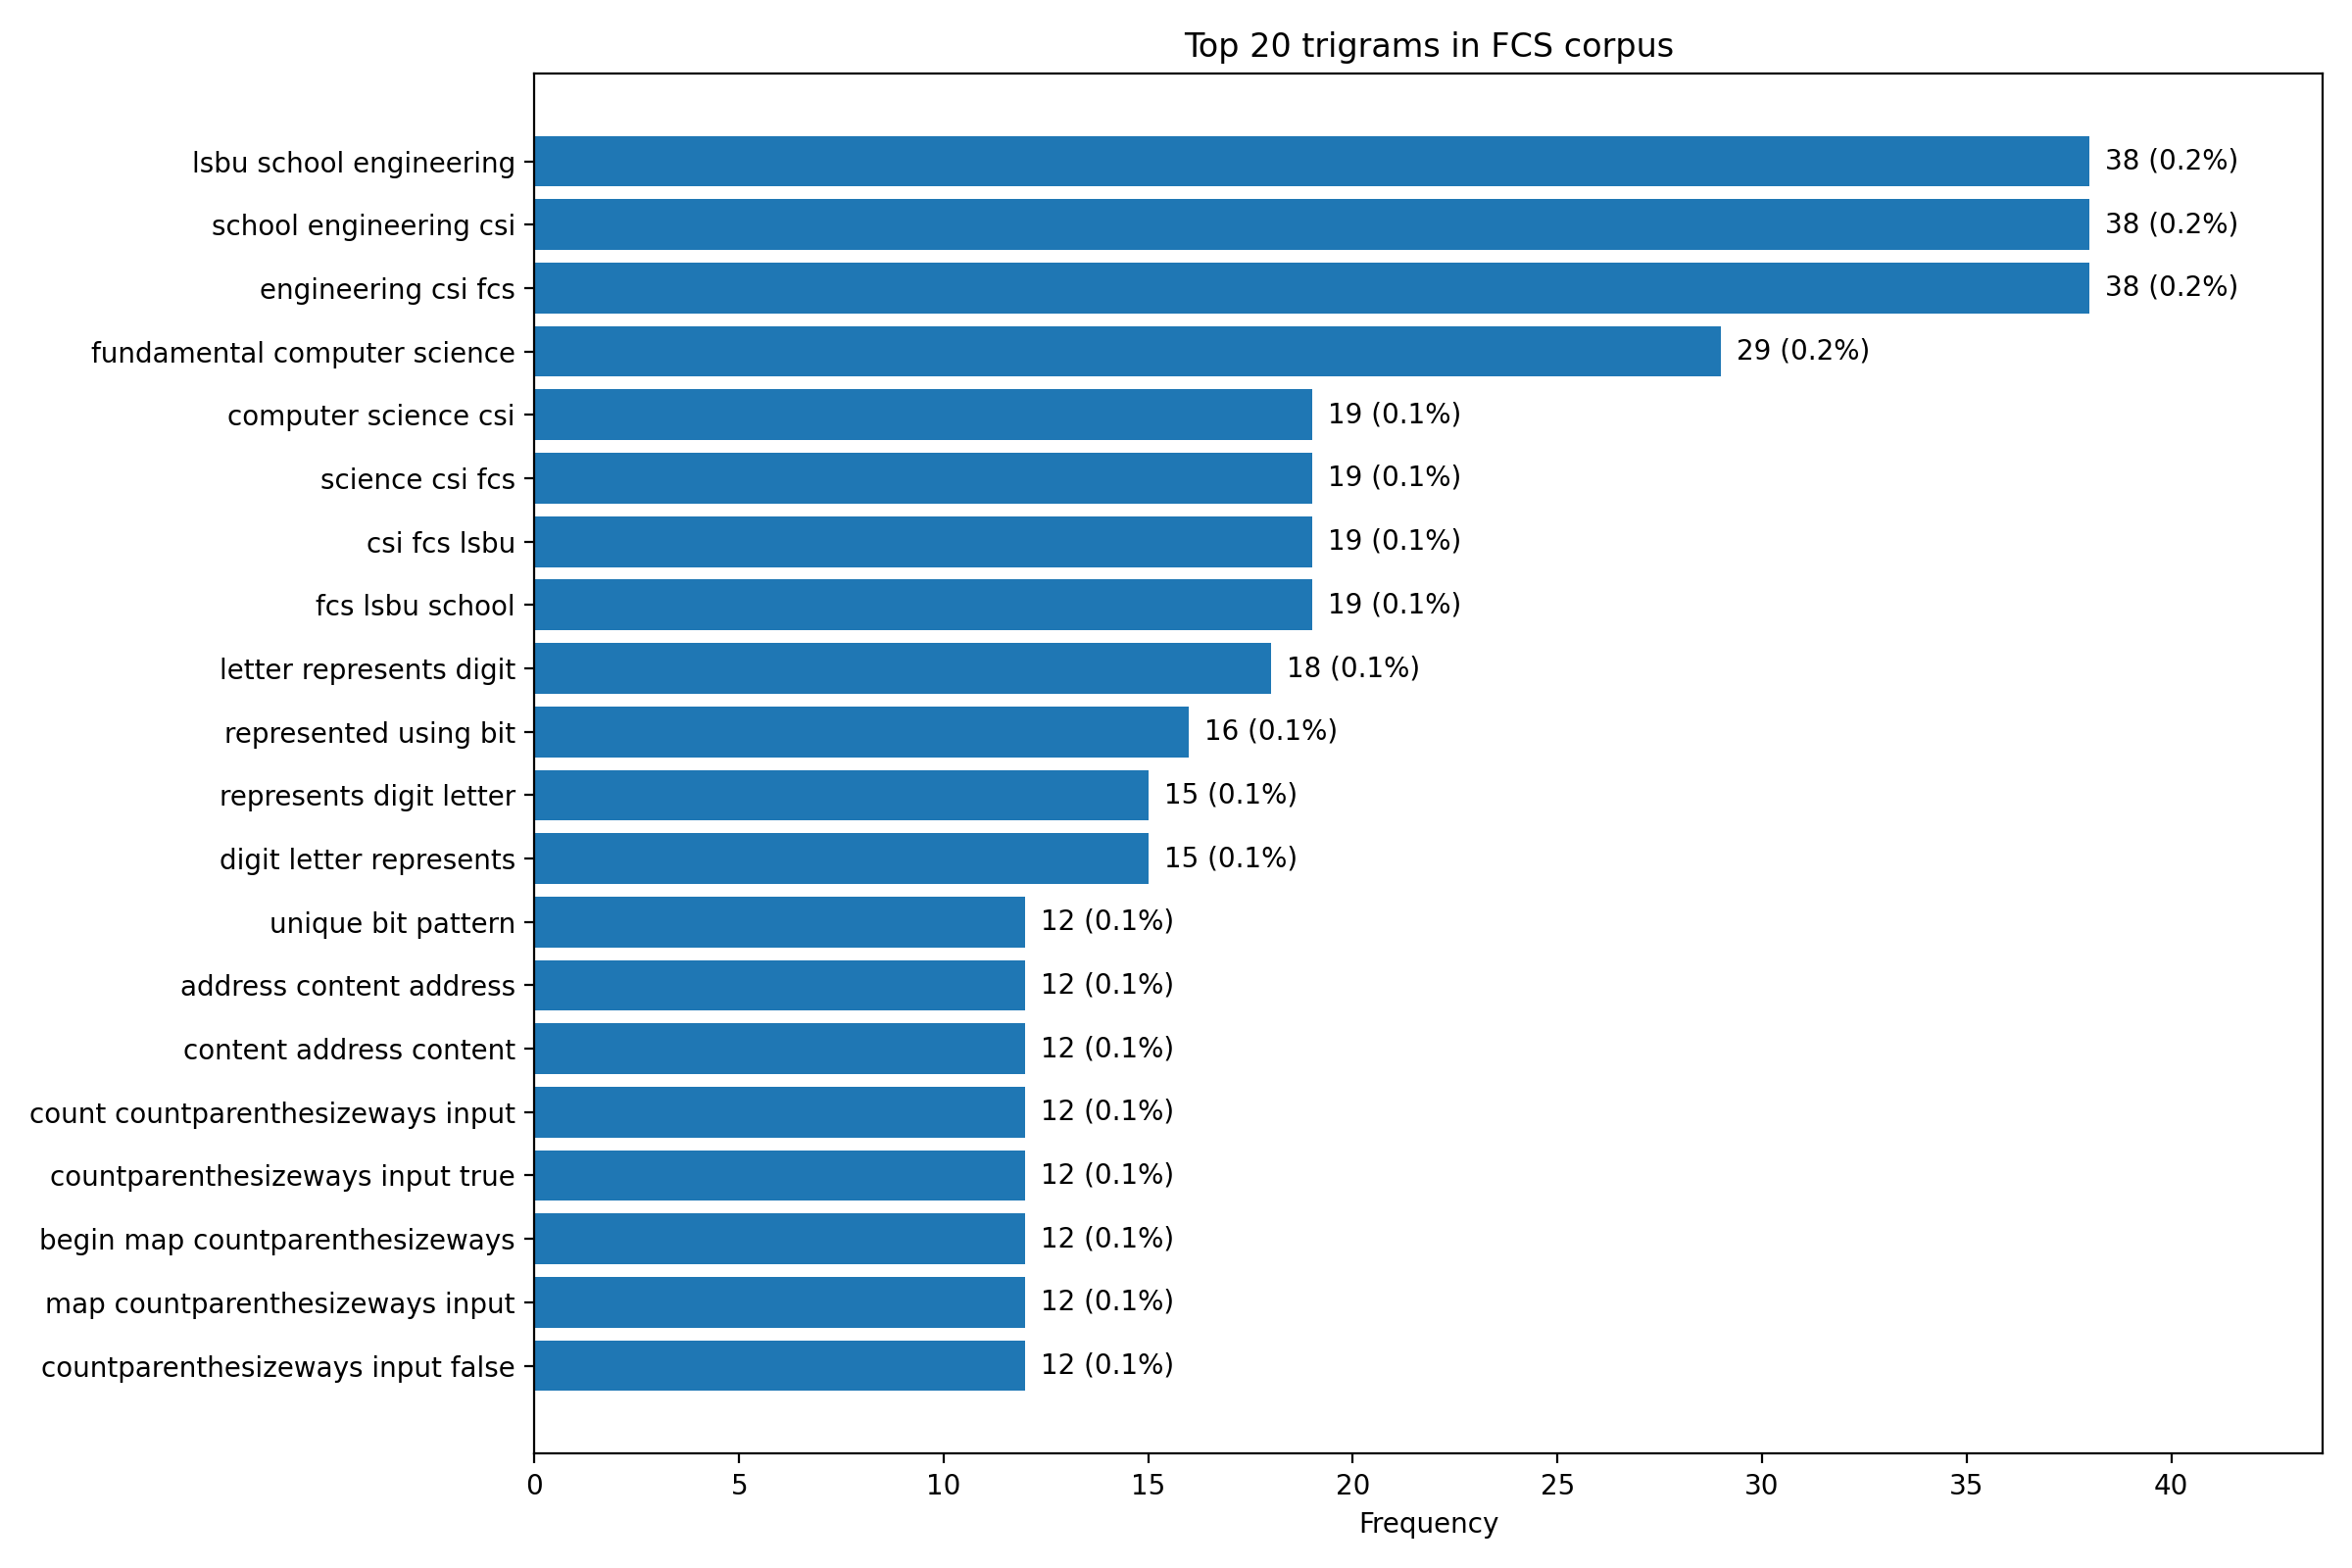
\includegraphics[width=\textwidth]{figs/FCS_top_trigrams.png}
    \caption{Top 20 trigrams in the FCS corpus.}
    \label{fig:fcs-trigrams}
\end{figure}
\FloatBarrier

For DMA, frequent words such as set, graph, vertex, edge, proposition, predicate and truth match the main topics of the module: set theory, logic and graph theory. However, frequent n-grams also include tutorial artefacts like "exercise page". These patterns describe the nature of the teaching materials, but may need extra cleaning if the goal is to focus only on conceptual content.

\begin{figure}[h]
    \centering
    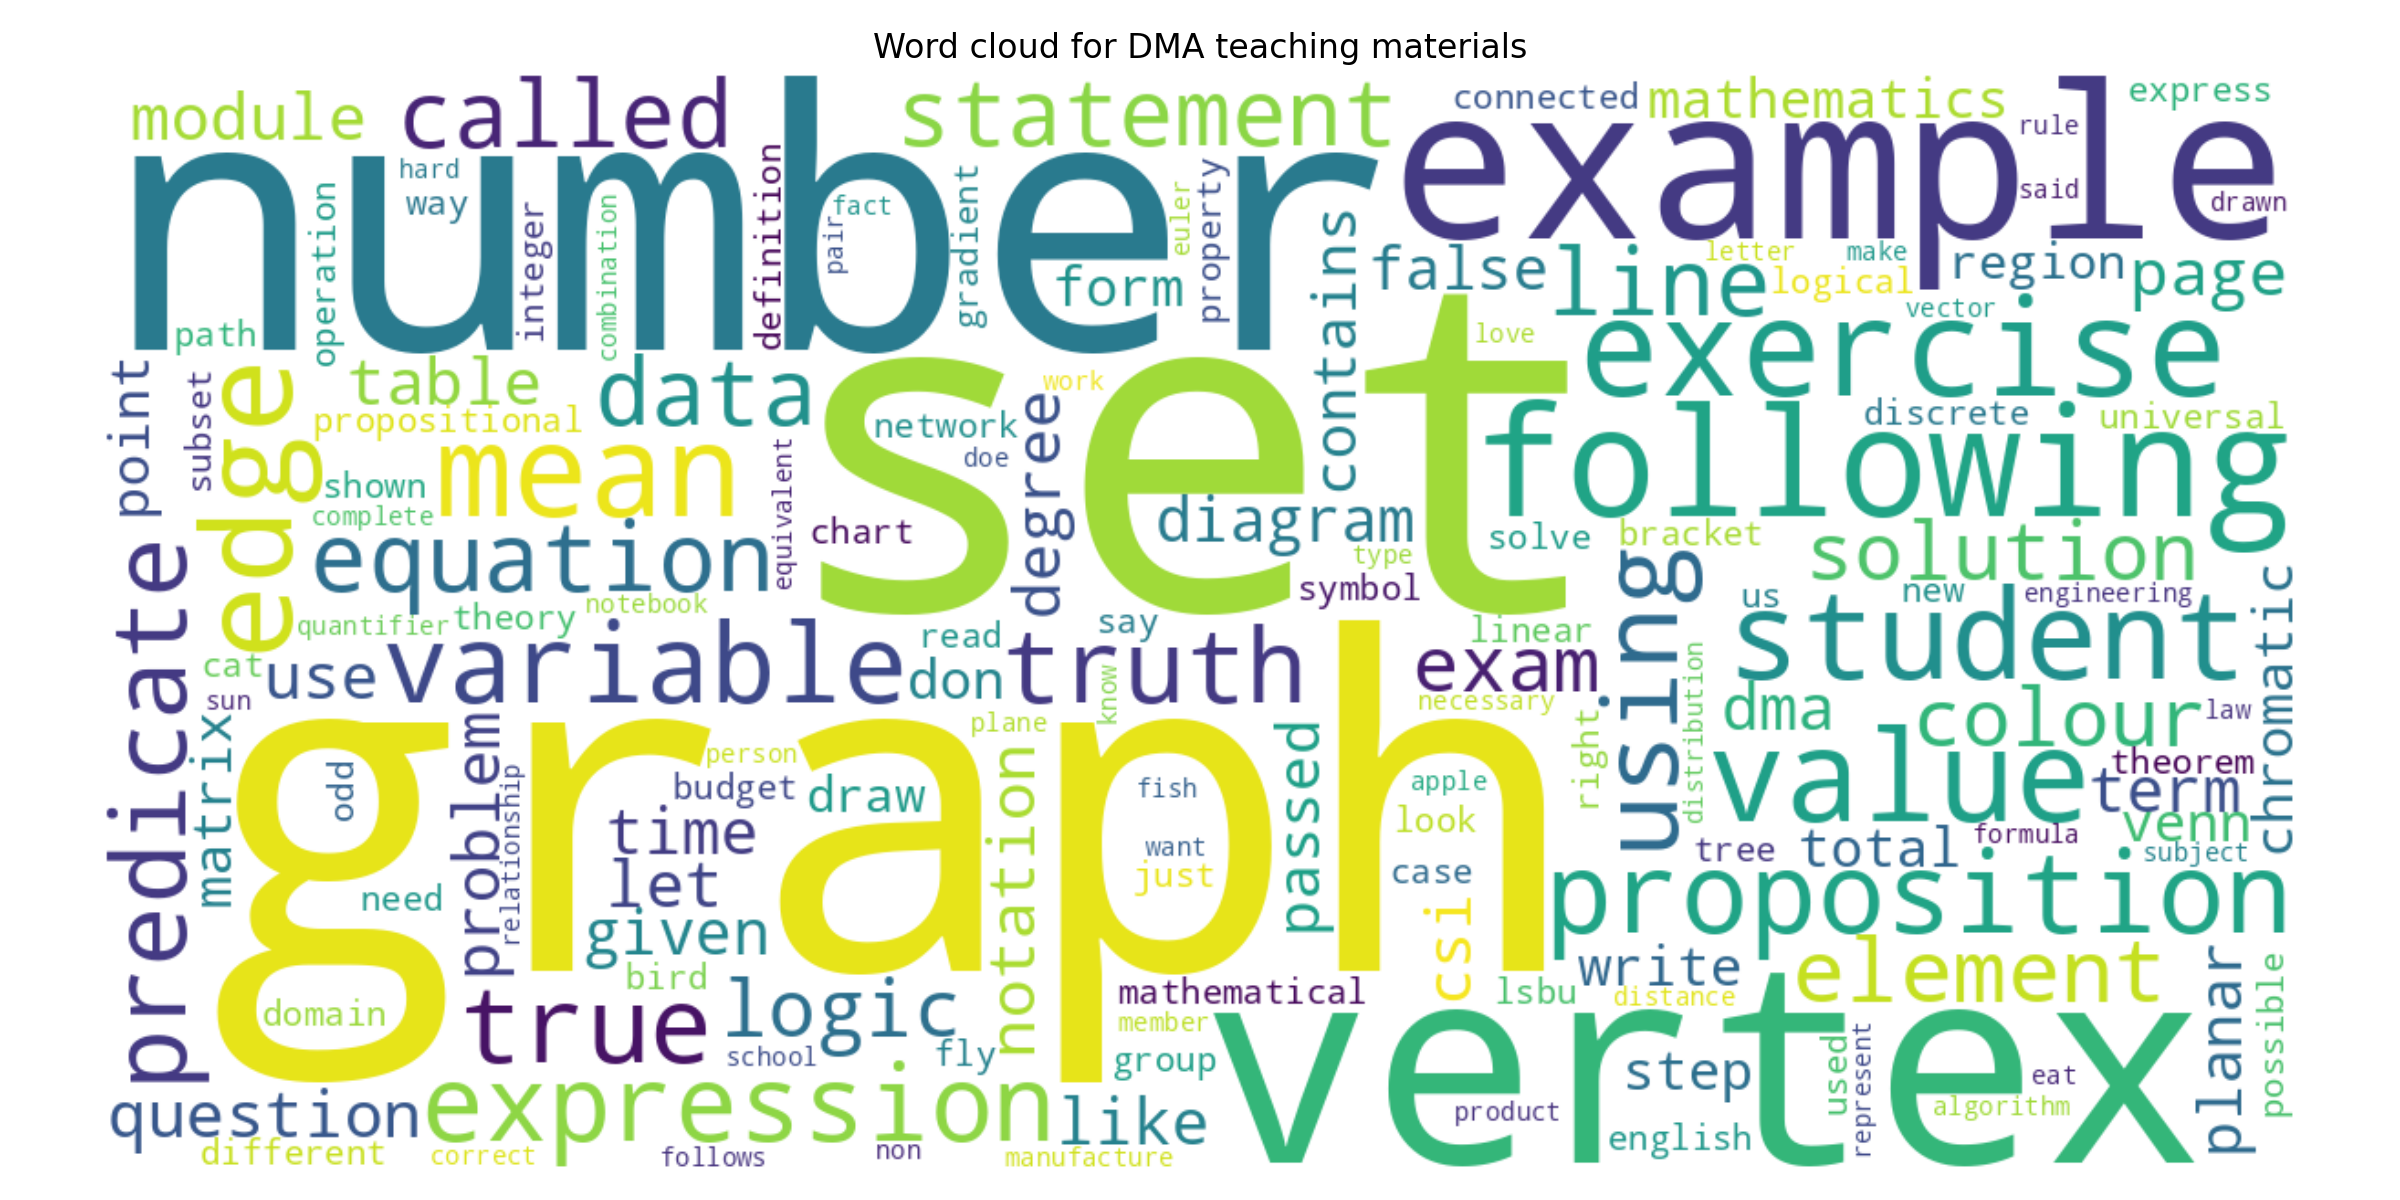
\includegraphics[width=\textwidth]{figs/DMA_wordcloud.png}
    \caption{Word cloud for the top content words in the DMA teaching materials.}
    \label{fig:dma-wordcloud}
\end{figure}
\FloatBarrier

\begin{figure}[h]
    \centering
    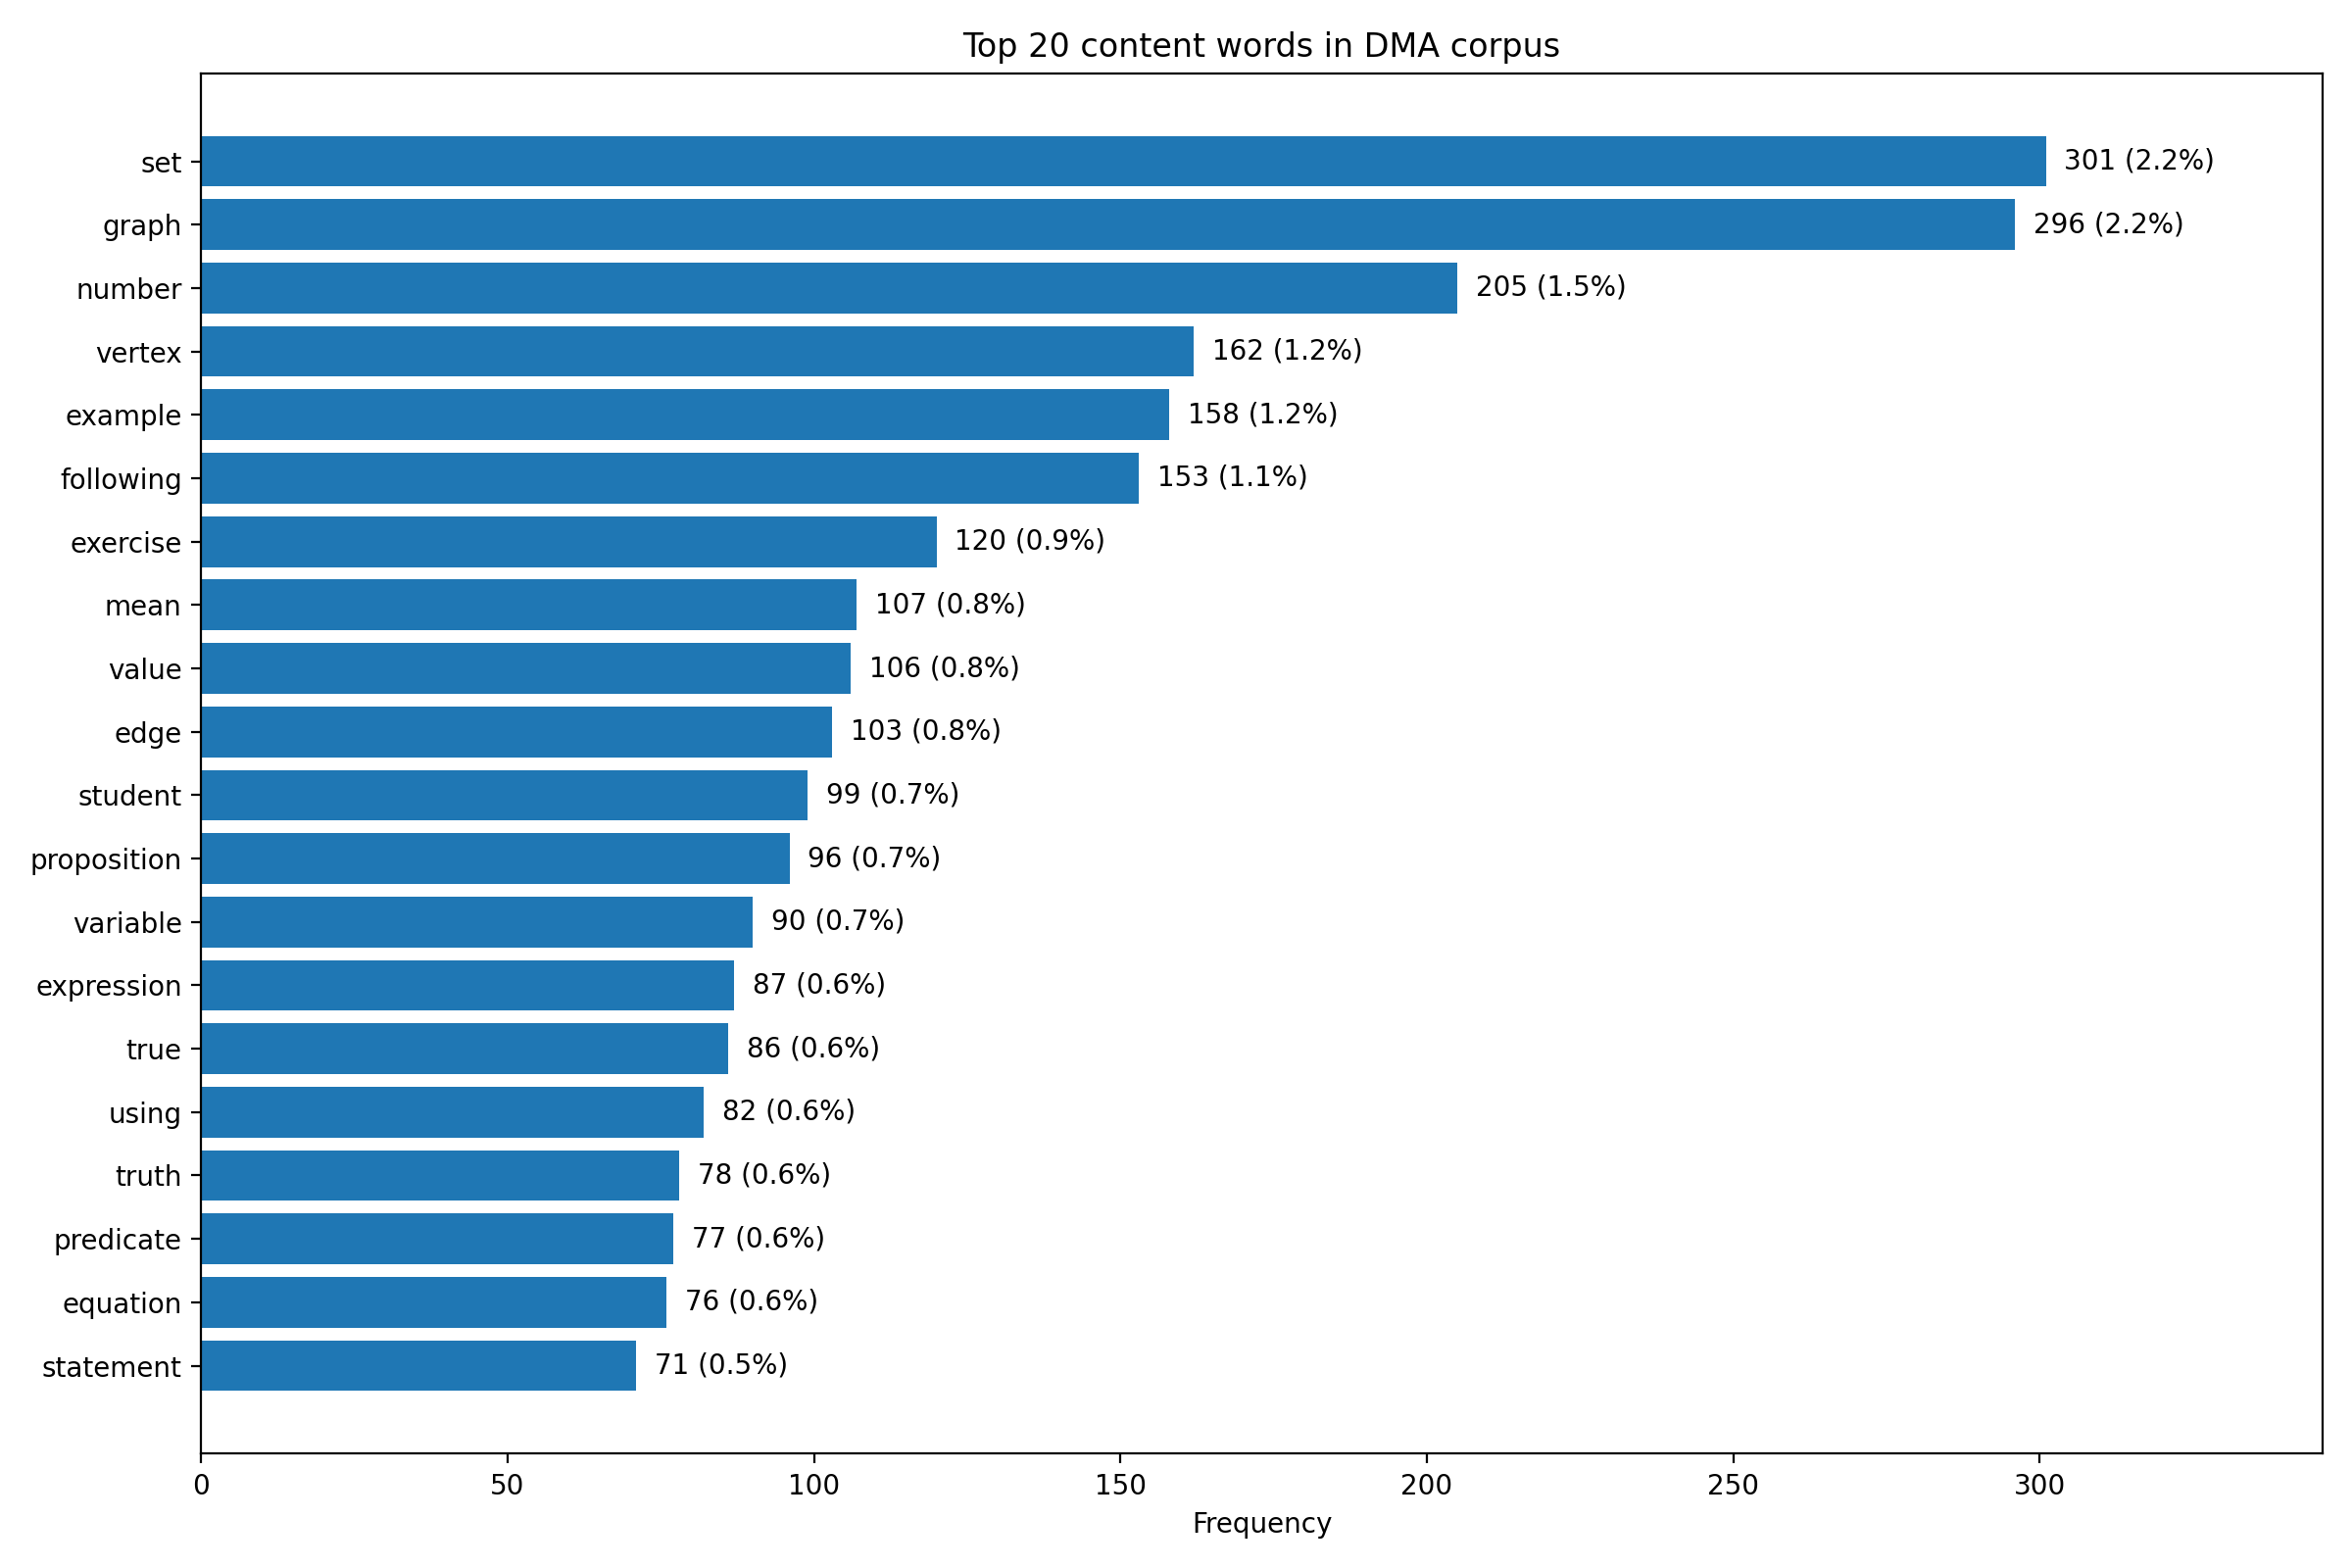
\includegraphics[width=\textwidth]{figs/DMA_top_words.png}
    \caption{Top 20 content words in the DMA corpus with their frequencies.}
    \label{fig:dma-topwords}
\end{figure}
\FloatBarrier

\begin{figure}[h]
    \centering
    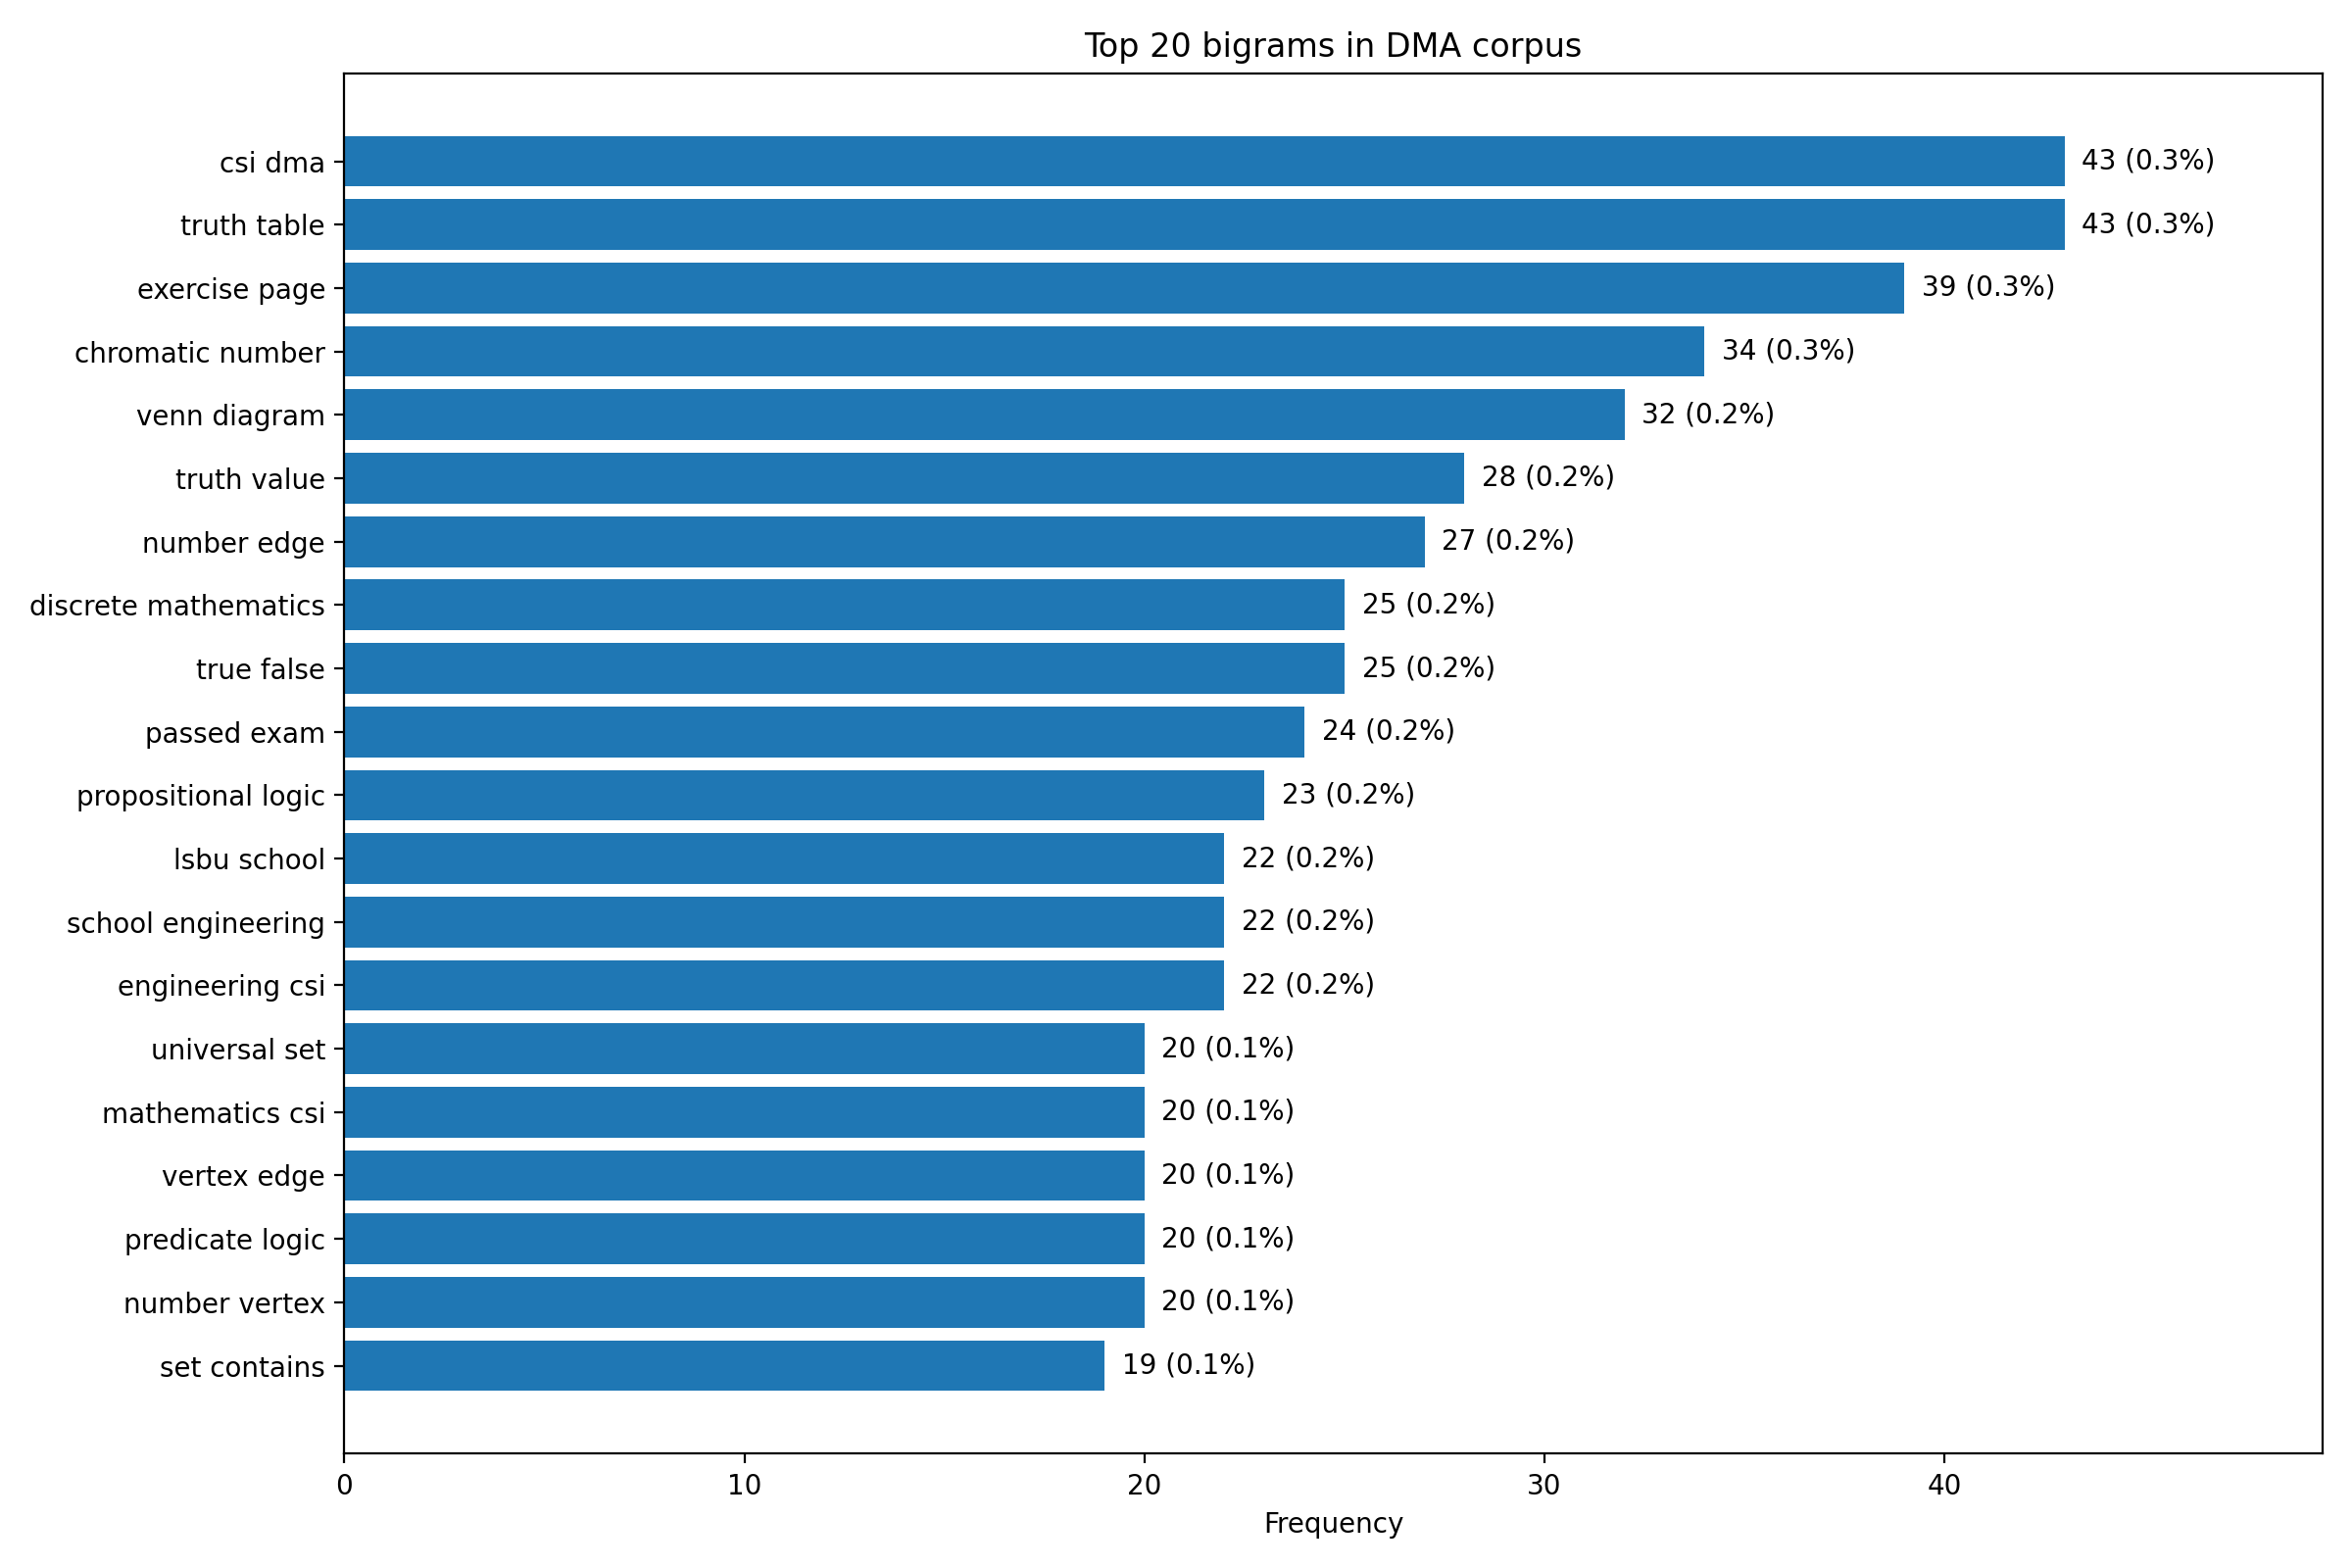
\includegraphics[width=\textwidth]{figs/DMA_top_bigrams.png}
    \caption{Top 20 bigrams in the DMA corpus.}
    \label{fig:dma-bigrams}
\end{figure}
\FloatBarrier

\begin{figure}[h]
    \centering
    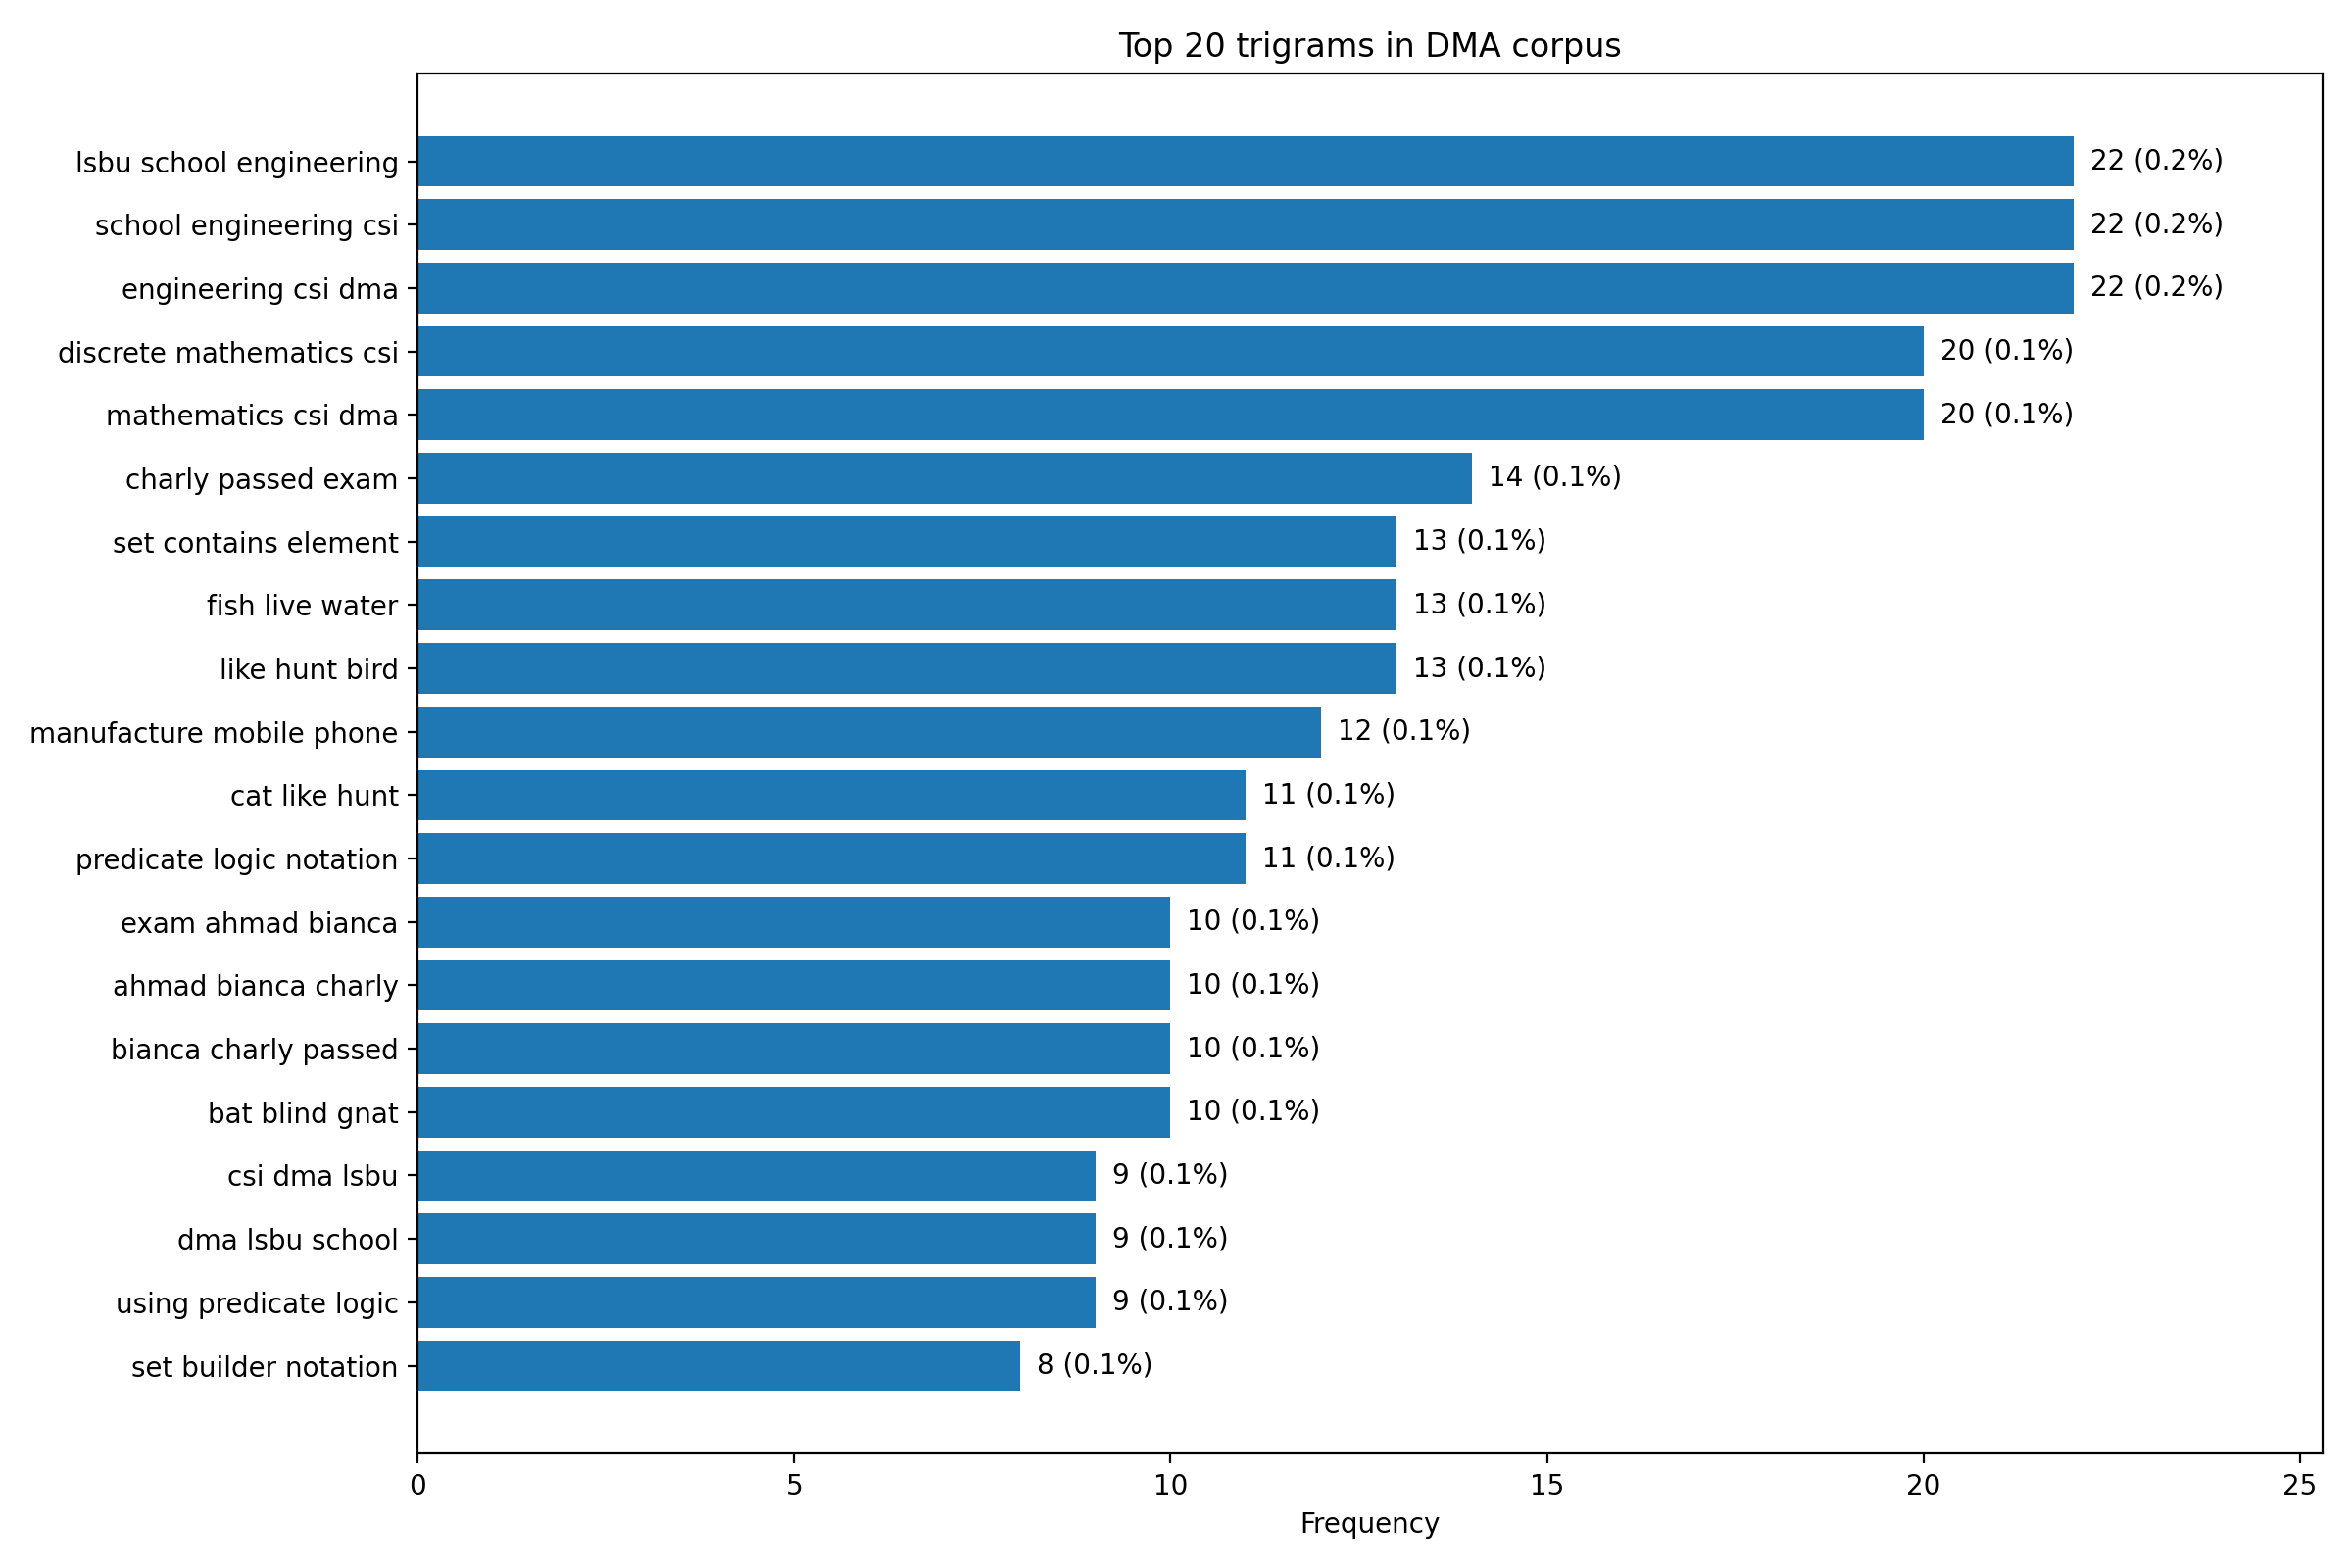
\includegraphics[width=\textwidth]{figs/DMA_top_trigrams.png}
    \caption{Top 20 trigrams in the DMA corpus.}
    \label{fig:dma-trigrams}
\end{figure}
\FloatBarrier

\paragraph{Normalising input into topic texts.}
All subject materials (PDF slides, PPTX lecture decks, and Word-based tutorials) were first consolidated into a unified intermediate representation stored as a topics.pkl file. Each entry is indexed by (subject, topic\_id) and contains the extracted text (full\_text) together with lightweight provenance metadata (a list of source\_files). This normalisation enables the same QA generation pipeline to be reused across subjects without relying on format-specific logic.

\subsection{Data preparation and preprocessing}

The teaching materials were transformed into a question-answer dataset suitable for training a small language model as an AI tutor. While the pipeline itself is subject-agnostic, model fine-tuning was performed separately for each subject. Three independent LoRA adapters were trained, one per subject, each using only the training data from its corresponding module.

\paragraph{Token-based chunking of long topics.}
Topic texts vary substantially in length. Tutorial sheets and consolidated notes can exceed the practical prompt budget for a small model. Therefore, each topic was split into overlapping chunks using the model tokenizer, with a target size of 1200 tokens and an overlap of 120 tokens. Chunks were limited to 1200 tokens to keep the full prompt (instructions + context) and the generated answer within the model’s 4096 token context window, while avoiding aggressive truncation and preserving space for multi-sentence tutor-style explanations. Chunking is performed on paragraph boundaries when possible, and oversized paragraphs are further split by sentence boundaries to avoid extremely long single segments. This step ensures that the model receives coherent context while leaving sufficient generation budget for explanatory answers.

\paragraph{Tutor-oriented QA generation.}
Question–answer pairs were generated using the microsoft/Phi-3-mini-4k-instruct model. The prompt was designed for a tutoring setting: answers are expected to be explanatory (not one-line definitions), typically spanning multiple sentences and focusing on understanding rather than rote memorisation. To increase coverage, the pipeline generates multiple question types per chunk using universal modes: core concepts, definitions and terms, application and reasoning, compare/contrast, and common mistakes. Since Phi-3-mini supports a 4k context window, the generation prompts were designed to fit within this budget (instructions + chunk context + answer). The target number of questions per chunk is chosen heuristically based on chunk length (4 for chunks under 300 tokens, 8 for 300-699 tokens, and 12 for chunks of over 700 tokens).

For each subject, the generated QA dataset was first split into training and evaluation subsets.
This split was performed before any automated or manual quality review to prevent information leakage between training and evaluation data. All subsequent processing steps, including GPT-based quality review and manual inspection, were applied independently to the training and evaluation splits.

\paragraph{Quality filtering.}
Because the target model is trained as an AI tutor, the dataset prioritises explanatory answers rather than one-line definitions. After generation, each candidate QA object is validated and filtered in several stages:

\begin{enumerate}
    \item \textbf{JSON validation and repair.} The model is instructed to output only a JSON array. The pipeline attempts strict JSON parsing. If parsing fails, it issues one repair prompt requesting JSON-only output. Outputs that remain unparsable after the retry are logged in qa\_errors\_<subject>.csv.
    \item 
    \item \textbf{Answer and question length filters.} Only QA pairs passing a deterministic quality function are retained. In particular, questions must contain at least 4 words and answers must contain at least 20 words to enforce tutor-style explanations.
    \item 
    \item \textbf{Deduplication.} To reduce redundancy within each subject, questions are normalised (lowercasing, whitespace normalisation, and punctuation removal) and normalised exact duplicates are removed. In the final datasets, the number of duplicate questions after normalisation is 0 for FSD, FCS and DMA.
    \item \textbf{Semi-automated quality review.} All generated QA pairs were reviewed using an automated GPT-based reviewer, which assigned each pair a label (OK or FLAGGED) together with optional reasons. To validate the reliability of this filtering step, random samples from both the OK and FLAGGED subsets were manually inspected. This inspection confirmed that the automated review reliably retained high-quality tutor-style explanations while filtering out low-quality or unsuitable examples.
    \item
\end{enumerate}

\paragraph{Evaluation subset used for metrics.}
For final metric reporting, only the evaluation subset labelled \texttt{OK} (saved as \texttt{<subject>\_eval\_OK.jsonl}) was used. This ensures that all reported scores are computed on high-quality tutor-style QA pairs and remain strictly held out from training.

\paragraph{Resulting QA datasets.}
The final datasets are stored as JSONL files (one QA pair per line) including metadata fields such as subject, topic\_id, chunk\_id, mode, and source\_files. The resulting dataset sizes are:
\begin{itemize}
    \item \textbf{FSD:} 680 QA pairs from 16 topics and 60 chunks (59 chunks used at least once), covering 31 source files.
    \item \textbf{FCS:} 745 QA pairs from 10 topics and 73 chunks (69 chunks used at least once), covering 32 source files.
    \item \textbf{DMA:} 708 QA pairs from 10 topics and 74 chunks (72 chunks used at least once), covering 25 source files.
\end{itemize}

\paragraph{Conversion to conversational fine-tuning format.}
For LoRA fine-tuning with Unsloth, the simple QA pairs are converted into a conversational format. A separate script reads the flat JSONL file with question-answer pairs and wraps each pair into a short conversation: a system message defining the tutor role for the subject, followed by the student question (user message) and the tutor answer (assistant message).

\section{Model development and training}
Although Phi-3-mini-4k-instruct was used for synthetic QA generation, model fine-tuning and evaluation were performed using microsoft/Phi-4-mini-instruct as the base model, with one LoRA adapter trained per subject (FSD, FCS, DMA). This keeps the training/evaluation stack consistent with the final inference setup used for metric reporting.


Model adaptation was performed separately for each subject. Starting from the same instruction-tuned
base model, three independent LoRA fine-tuning runs were executed, resulting in subject-specific
adapters for FSD, FCS, and DMA. This design choice allows each model to specialise in the terminology, problem types, and explanatory style of its corresponding module, while preserving a consistent training and evaluation methodology across subjects.

The goal of the Agentic AI Tutor is to adapt an existing instruction-tuned model to a specific academic tutoring domain. Low-Rank Adaptation (LoRA) was selected as the main fine-tuning method. The implementation follows best practices described in the Unsloth documentation \parencite{LoRAfine55:online} and uses the Unsloth training framework and example notebooks \parencite{GitHubun10:online} as a reference for stable and efficient fine-tuning.

\subsection{LoRA configuration}

The LoRA configuration was chosen based on recommendations from the Unsloth hyperparameter guide \parencite{LoRAfine55:online} and preliminary experiments. The following key settings were used:

\begin{itemize}
    \item \textbf{LoRA rank ($r=16$).} This value provides sufficient capacity for domain adaptation while keeping the number of trainable parameters low.
    \item \textbf{LoRA scaling factor ($\alpha=16$).} Setting $\alpha$ equal to the rank follows a commonly recommended heuristic and results in stable training behaviour.
    \item \textbf{Target modules.} LoRA adapters were applied to all major linear layers in both the attention and feed-forward blocks (query, key, value, output, and MLP projections). This ensures that the model can adapt both its attention patterns and its internal representations.
    \item \textbf{LoRA dropout ($0.0$).} Dropout was disabled, as the fine-tuning runs are short and the dataset is already filtered for quality.
    \item \textbf{Bias training.} Bias terms were not trained to reduce unnecessary parameter updates.
\end{itemize}

Gradient checkpointing provided by Unsloth was enabled to further reduce memory consumption during training.

\subsection{Training setup}

The training configuration was designed to achieve a stable effective batch size while remaining within GPU memory limits. The main parameters are:

\begin{itemize}
    \item \textbf{Per-device batch size:} 2
    \item \textbf{Gradient accumulation steps:} 8
    \item \textbf{Effective batch size:} 16
    \item \textbf{Learning rate:} $2 \times 10^{-4}$
    \item \textbf{Weight decay:} 0.01
    \item \textbf{Warm-up ratio:} 5\%
    \item \textbf{Number of epochs:} 1
\end{itemize}

An effective batch size of 16 is recommended in the Unsloth documentation as a good default for stable fine-tuning of instruction-based datasets. Training for a single epoch was chosen to reduce the risk of overfitting, as the dataset consists of synthetic but carefully filtered tutor-style question-answer pairs.

\subsection{Design choice: training without response-only masking}

Some fine-tuning pipelines apply loss masking so that the model is trained only on assistant tokens, ignoring system and user messages. While this technique can be useful for large multi-turn conversational datasets, it was deliberately not used in this project.

During implementation, applying response-only masking caused all training labels to be masked out due to strict token-level matching requirements in the training framework. More importantly, the dataset used in this project consists exclusively of single-turn tutor-style interactions with a clear and consistent structure. In this setting, training on the full input sequence does not introduce significant noise and simplifies the training pipeline.

For these reasons, the final implementation keeps the training code unchanged and performs standard supervised fine-tuning without response-only masking. This decision improves robustness and reproducibility while preserving the intended tutoring behaviour of the model.

\subsection{Training environment}

All fine-tuning experiments were conducted in Google Colab using a free NVIDIA Tesla T4 GPU. The Unsloth framework was used to optimise memory usage and training speed.

The trained model is saved as LoRA adapter weights. This allows the adapters to be reused with the original base model during inference, or merged into a standalone model if required for deployment.

\subsection{Retrieval-Augmented Generation}

In addition to fine-tuning the base model with LoRA adapters, the Agentic AI Tutor supports retrieval-augmented generation (RAG) to ground its answers in the original teaching materials.

The RAG pipeline reuses the same token-based chunks created during the data preparation stage. Instead of treating full lecture or tutorial files as retrieval units, each subject corpus is indexed at the chunk level. This design choice is motivated by a factor that semantic retrieval performs better when embeddings represent short, topically coherent text segments rather than long documents containing multiple concepts.

Each retrieved chunk retains lightweight provenance metadata, including the topic identifier and source file names. This allows the system to trace answers back to specific lecture slides or tutorial documents, which is useful for debugging, evaluation, and future user-facing citation features.

For each subject (FSD, FCS and DMA), all chunks are embedded using a lightweight sentence-transformer model and stored in a persistent vector database (ChromaDB). The RAG component operates independently of fine-tuning.

\section{Model evaluation and testing}

Model quality was evaluated separately for each subject (FSD, FCS, DMA) using the corresponding eval\_OK subset. This evaluation set contains only question-answer pairs that passed the semi-automated GPT-based quality review and subsequent manual spot-checking.

We compared five model variants:
\begin{itemize}
    \item \textbf{BASE}: the instruction-tuned base model without adaptation,
    \item \textbf{LoRA}: the base model with a subject-specific LoRA adapter,
    \item \textbf{LoRA+RAG}: the LoRA-adapted model augmented with retrieval of subject materials,
    \item \textbf{Qwen3-32B}: an external LLM baseline,
    \item \textbf{Llama-70B}: an external LLM baseline.
\end{itemize}

All metrics were computed within each subject (FSD/FCS/DMA) using the same evaluation script and the same prompt format. Each model answer was compared to the held-out reference tutor answer.

\subsection{Metrics}
To measure answer quality, we use both lexical overlap metrics (how much the text matches the reference wording) and a semantic similarity metric (how similar the meaning is even if the wording changes). We also report runtime (latency). Lexical-overlap metrics (BLEU, ROUGE-L, METEOR) reward shared words and phrases, so they are sensitive to paraphrasing. Semantic similarity (BERTScore) is more robust to paraphrase. It can increase even if lexical overlap stays modest.

\begin{table}[h]
\centering
\caption{Metric units and value ranges used in this evaluation.}
\label{tab:metric-units-ranges}
\small
\resizebox{\linewidth}{!}{%
\begin{tabular}{lll}
\toprule
\textbf{Metric} & \textbf{Units} & \textbf{Typical range} \\
\midrule
BLEU-2 & Percent scale & 0-100 \\
ROUGE-L & Fraction (float) & 0.0-1.0 \\
METEOR & Fraction (float) & 0.0-1.0 \\
BERTScore F1 & Fraction (float), rescaled & 0.0-1.0 \\
Latency (mean / median) & Seconds & No fixed range \\
\bottomrule
\end{tabular}}
\end{table}
\FloatBarrier

\paragraph{BLEU (lexical overlap).}
BLEU measures modified n-gram precision between a candidate answer and a reference answer, with a brevity penalty for very short outputs \parencite{BleuaMet4:online}. In this project, BLEU is reported on a 0-100 scale. In tutoring-style answers, BLEU is usually low because there are many correct ways to explain the same idea.

\paragraph{ROUGE-L (lexical overlap).}
ROUGE-L is based on the longest common subsequence (LCS) between candidate and reference \parencite{ROUGEAPa16:online}. It is reported in the 0-1 range: 1 means identical text order, 0 means no overlap in sequence.

\paragraph{METEOR (lexical overlap with flexible matching).}
METEOR aligns candidate and reference using unigram matches (including stemming and synonymy) and combines precision and recall with a fragmentation penalty \parencite{METEORAn22:online}. It is also reported in the 0-1 range.

\paragraph{BERTScore F1 (semantic similarity).}
BERTScore compares candidate and reference using contextual embeddings and reports F1 similarity \parencite{Zhang2019BERTScore}. Higher values mean the meaning is closer even if words differ. 

\paragraph{Latency.}
Latency is reported as mean and median inference time per example (seconds). Lower is better.

\subsection{Results}

Tables \ref{tab:metrics-fsd}-\ref{tab:metrics-dma} report the evaluation results for each subject.

\paragraph{Colour coding (SLM variants only).}
In the tables below, colour is applied only within the three local variants: BASE, LoRA, and LoRA+RAG.
For each metric column:
\begin{itemize}
    \item \textcolor{blue}{Blue} marks the \textbf{best} value among BASE/LoRA/LoRA+RAG.
    \item \textcolor{red}{Red} marks the \textbf{worst} value among BASE/LoRA/LoRA+RAG.
\end{itemize}
For quality metrics (BLEU, ROUGE-L, METEOR, BERTScore F1), \textbf{higher is better}.
For latency (mean/median seconds), \textbf{lower is better}.

\begin{table}[h]
\centering
\caption{Evaluation metrics on \texttt{eval\_OK} for FSD (SLMs vs.\ LLM baselines).}
\label{tab:metrics-fsd}
\small
\resizebox{\linewidth}{!}{%
\begin{tabular}{lrrrrrr}
\toprule
Model & BLEU & ROUGE-L & METEOR & BERTScore F1 & Latency (mean) & Latency (median) \\
\midrule
BASE     & \worst{5.260}  & \worst{0.129} & \best{0.297}  & \worst{0.062} & \best{27.116} & \best{26.808} \\
LoRA     & 10.028         & 0.186         & \worst{0.263} & \best{0.257}  & 29.050        & 28.833 \\
LoRA+RAG & \best{11.161}  & \best{0.209}  & 0.268         & 0.242         & \worst{29.493}& \worst{29.041} \\
\midrule
LLM (Llama-3.3-70B) & 8.958 & 0.212 & 0.310 & 0.194 & 2.475 & 2.647 \\
LLM (Qwen3-32B)     & 7.761 & 0.155 & 0.301 & 0.153 & 2.527 & 2.687 \\
\bottomrule
\end{tabular}
}
\end{table}
\FloatBarrier


\begin{table}[h]
\centering
\caption{Evaluation metrics on \texttt{eval\_OK} for FCS (SLMs vs.\ LLM baselines).}
\label{tab:metrics-fcs}
\small
\resizebox{\linewidth}{!}{%
\begin{tabular}{lrrrrrr}
\toprule
Model & BLEU & ROUGE-L & METEOR & BERTScore F1 & Latency (mean) & Latency (median) \\
\midrule
BASE     & \worst{6.296}  & \worst{0.138} & \best{0.291}  & \worst{0.089} & \best{27.393} & \best{27.158} \\
LoRA     & 11.810         & \best{0.211}  & 0.253         & \best{0.272}  & 29.279        & 28.827 \\
LoRA+RAG & \best{12.105}  & 0.210         & \worst{0.238} & 0.247         & \worst{29.540}& \worst{29.191} \\
\midrule
LLM (Llama-3.3-70B) & 11.617 & 0.237 & 0.346 & 0.243 & 2.553 & 2.649 \\
LLM (Qwen3-32B)     & 8.937  & 0.166 & 0.317 & 0.152 & 2.612 & 2.697 \\
\bottomrule
\end{tabular}
}
\end{table}
\FloatBarrier

\begin{table}[h]
\centering
\caption{Evaluation metrics on \texttt{eval\_OK} for DMA (SLMs vs.\ LLM baselines).}
\label{tab:metrics-dma}
\small
\resizebox{\linewidth}{!}{%
\begin{tabular}{lrrrrrr}
\toprule
Model & BLEU & ROUGE-L & METEOR & BERTScore F1 & Latency (mean) & Latency (median) \\
\midrule
BASE     & \worst{5.851}  & \worst{0.130} & \best{0.291}  & \worst{0.082} & \best{26.433} & \best{25.985} \\
LoRA     & 9.282          & 0.196         & \worst{0.255} & 0.208         & 28.444        & 27.638 \\
LoRA+RAG & \best{10.293}  & \best{0.203}  & 0.263         & \best{0.218}  & \worst{28.829}& \worst{28.390} \\
\midrule
LLM (Llama-3.3-70B) & 9.805 & 0.211 & 0.337 & 0.211 & 2.599 & 2.661 \\
LLM (Qwen3-32B)     & 7.595 & 0.152 & 0.299 & 0.120 & 2.525 & 2.665 \\
\bottomrule
\end{tabular}
}
\end{table}
\FloatBarrier

\subsection{Analysis}

\paragraph{How to read the numbers.}
BLEU and ROUGE-L are lexical-overlap metrics. They reward using the same words and similar word order as the single reference tutor answer. BLEU is reported on a 0-100 scale (here mostly 5-12 for SLMs), so low absolute values mainly mean limited exact phrase overlap, which is normal when many correct tutor-style phrasings exist. ROUGE-L (0-1) measures the longest common subsequence. Values around 0.13-0.22 indicate modest in-sequence overlap for multi-sentence explanations. METEOR (0-1) uses unigram matching (including flexible matching such as stemming/synonymy) and adds a penalty when matched words appear in fragmented order. Values around 0.24-0.30 here mean partial alignment to the reference. BERTScore F1 is a semantic-similarity metric. Higher values indicate stronger meaning similarity even when surface wording differs. In this project BERTScore is reported in a rescaled form.

\paragraph{BASE vs.\ LoRA (effect of fine-tuning).}
Figure \ref{fig:all-bleu} and Figure \ref{fig:all-bertscore} summarise the main improvements from BASE to LoRA across subjects.

\begin{figure}[h]
    \centering
    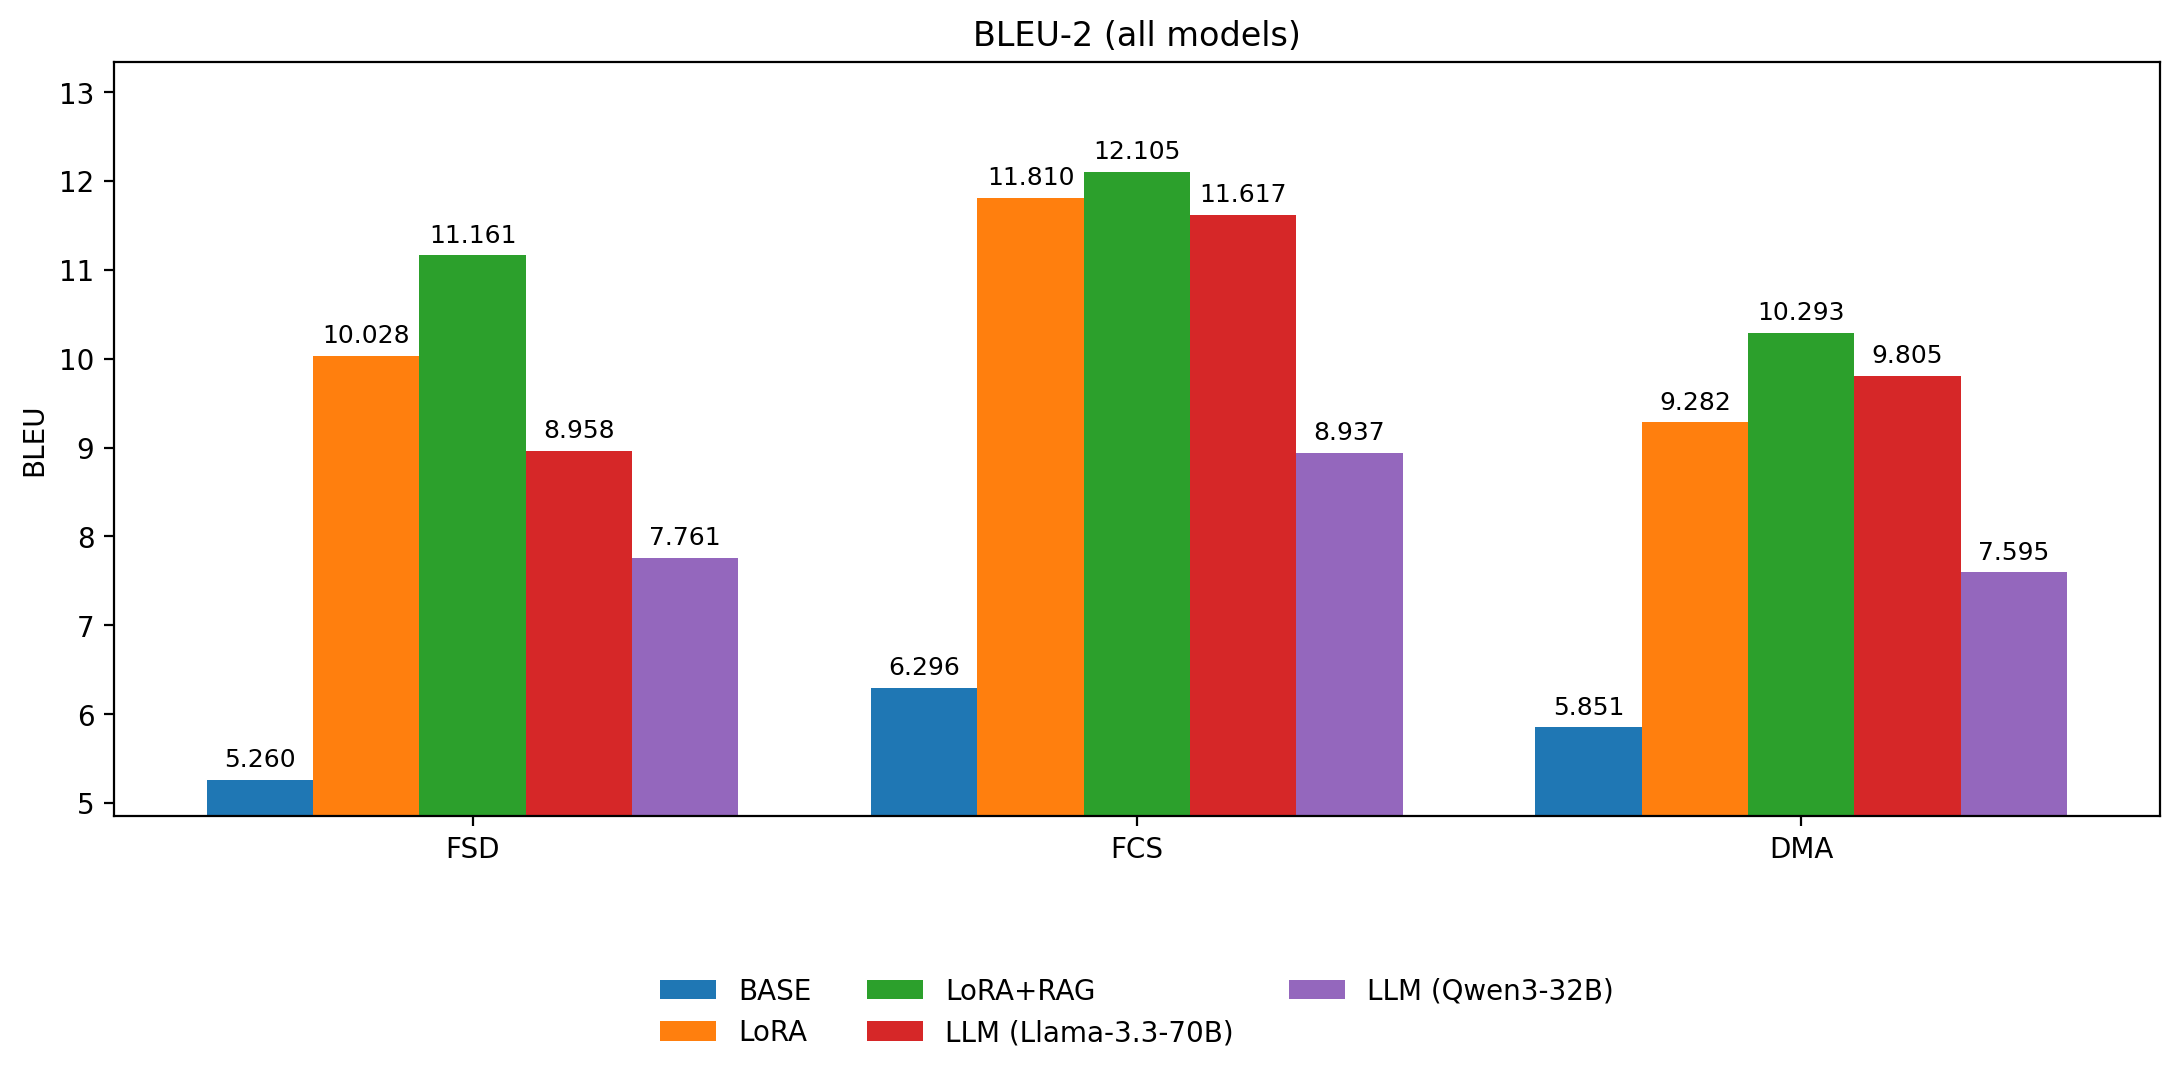
\includegraphics[width=\linewidth]{figs/all_bleu.png}
    \caption{BLEU-2 across subjects for all models.}
    \label{fig:all-bleu}
\end{figure}

\begin{figure}[h]
    \centering
    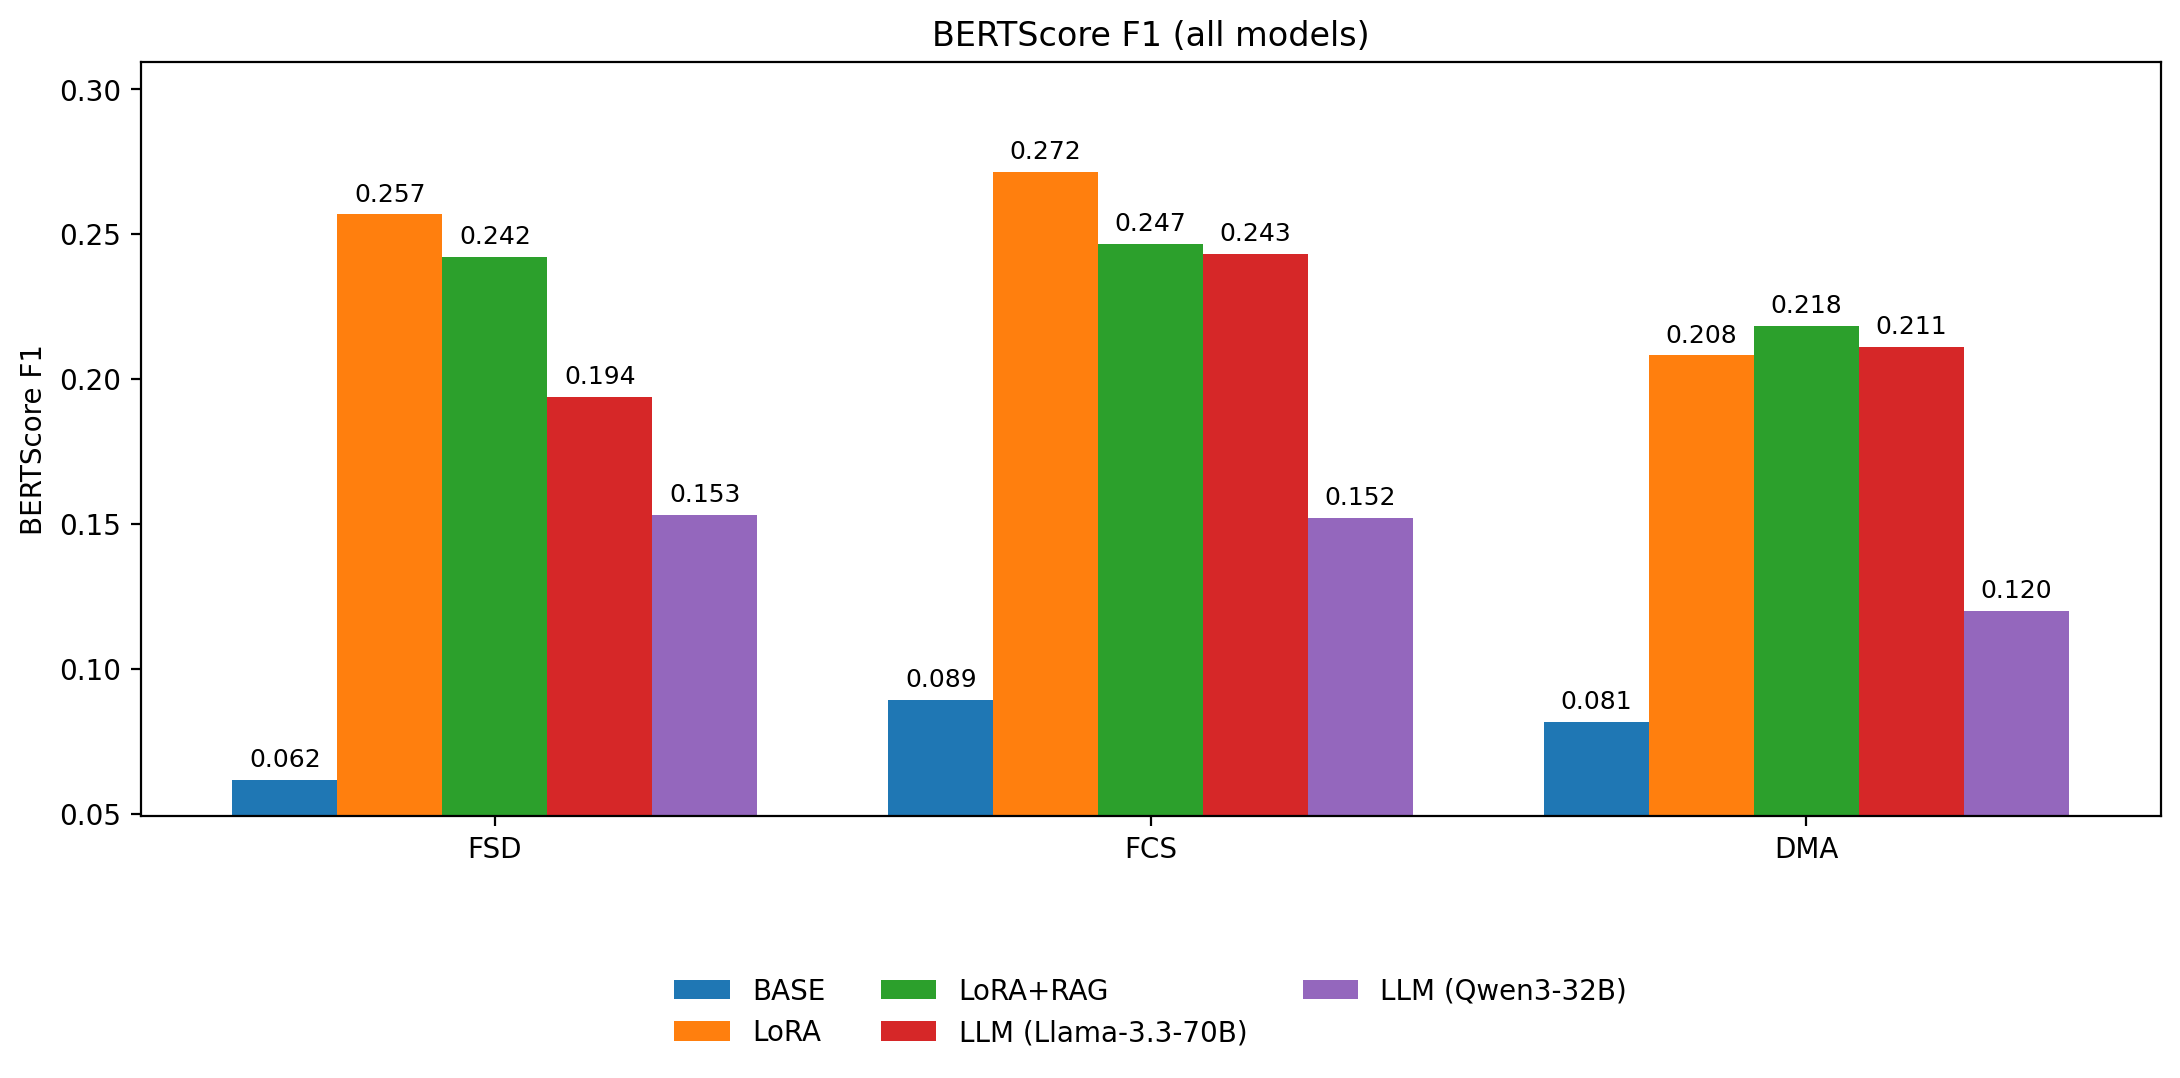
\includegraphics[width=\linewidth]{figs/all_bertscore.png}
    \caption{BERTScore F1 across subjects for all models.}
    \label{fig:all-bertscore}
\end{figure}
\FloatBarrier

Across all three subjects, LoRA improves BLEU-2, ROUGE-L, and BERTScore compared to BASE:
\begin{itemize}
    \item \textbf{FSD:} BLEU-2 increases from 5.260 to 10.028, ROUGE-L from 0.129 to 0.186, and BERTScore F1 from 0.062 to 0.257.
    \item \textbf{FCS:} BLEU-2 increases from 6.296 to 11.810, ROUGE-L from 0.138 to 0.211, and BERTScore F1 from 0.089 to 0.272.
    \item \textbf{DMA:} BLEU-2 increases from 5.851 to 9.282, ROUGE-L from 0.130 to 0.196, and BERTScore F1 from 0.082 to 0.208.
\end{itemize}
These gains mean the LoRA adapters help the SLM follow subject terminology and produce explanations that are closer to the reference answers both in surface form (BLEU-2/ROUGE-L) and in meaning (BERTScore).

\paragraph{LoRA vs.\ LoRA+RAG (effect of retrieval).}
Figure \ref{fig:all-rougeL} helps to see that ROUGE-L gains from retrieval are smaller and sometimes mixed.

\begin{figure}[h]
    \centering
    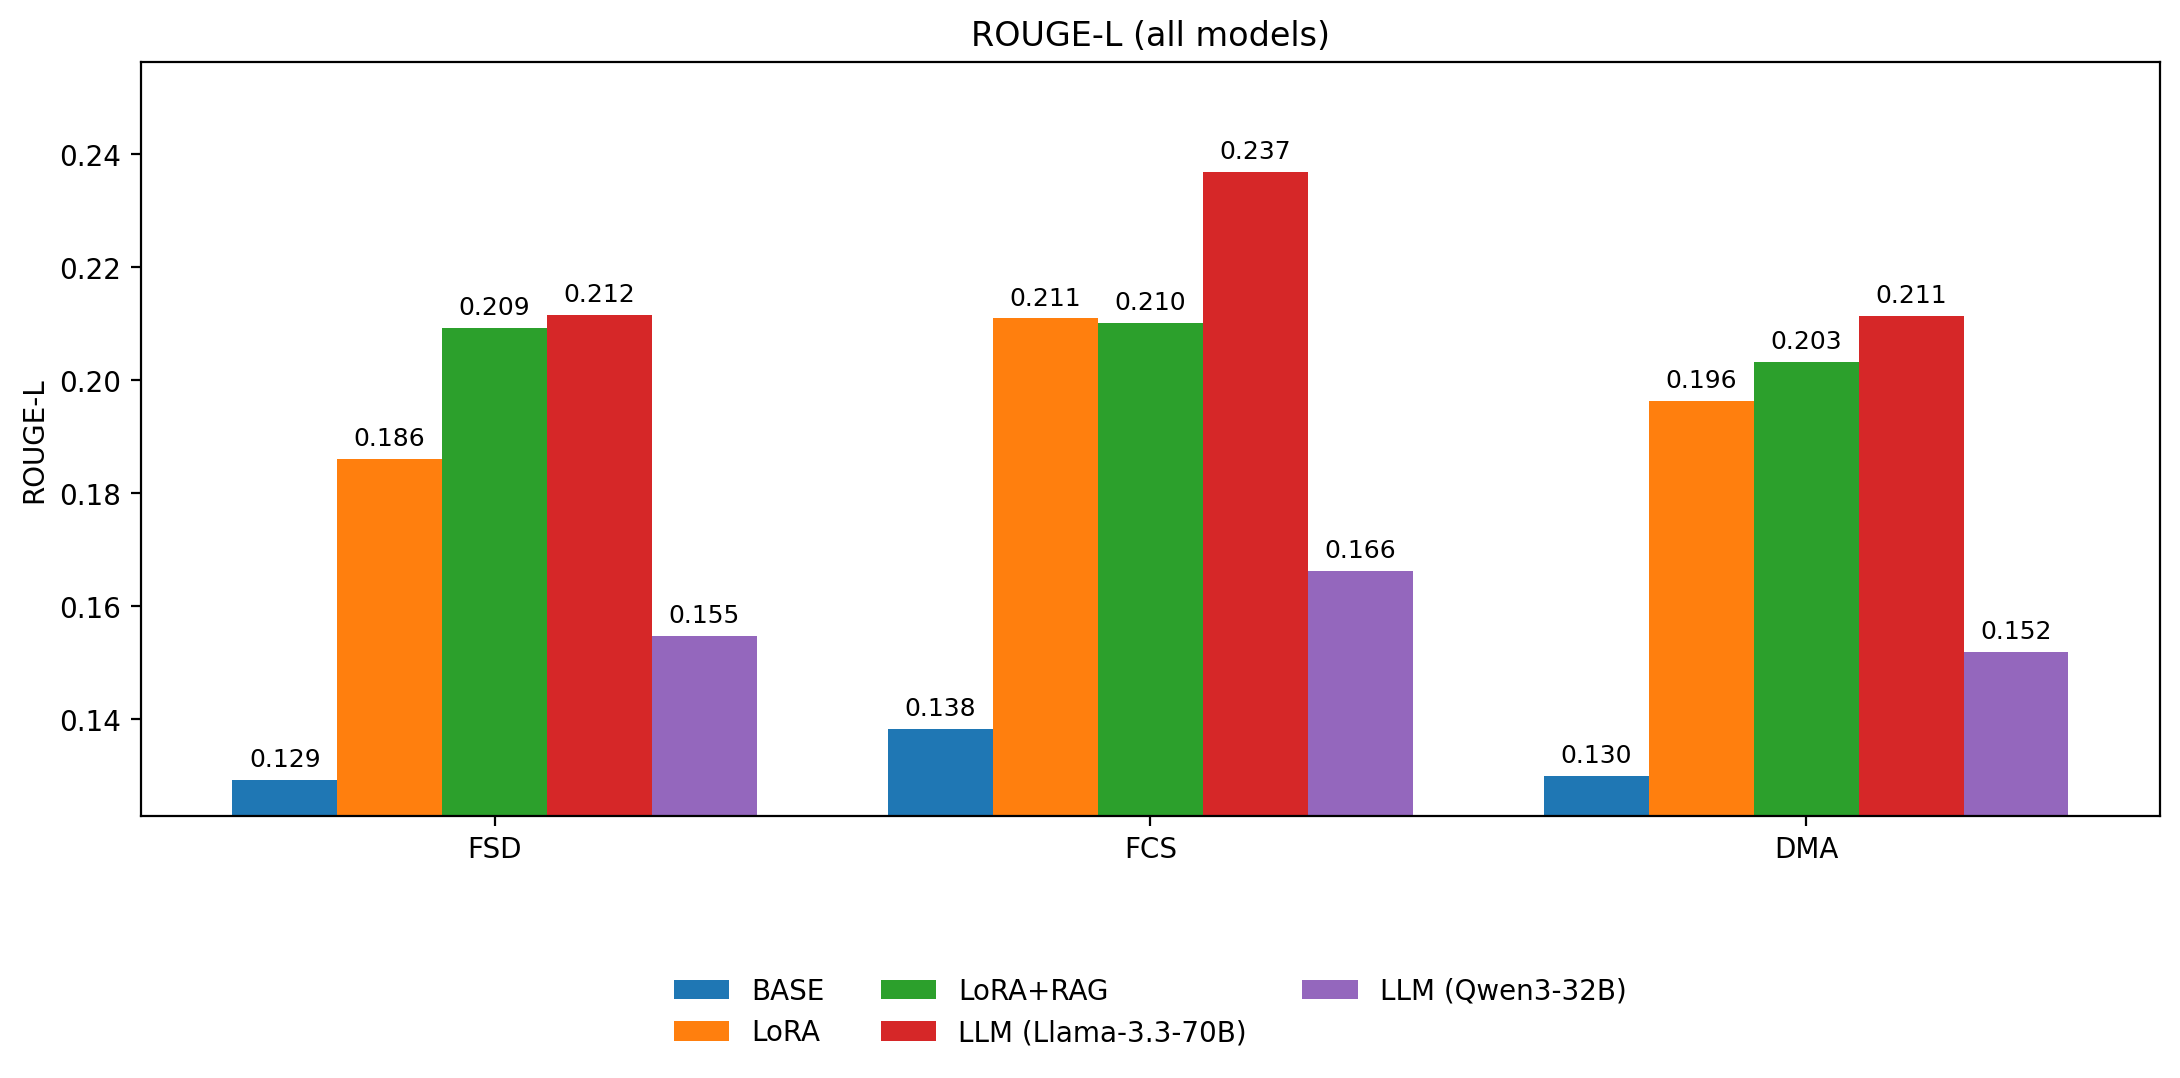
\includegraphics[width=\linewidth]{figs/all_rougeL.png}
    \caption{ROUGE-L across subjects for all models.}
    \label{fig:all-rougeL}
\end{figure}
\FloatBarrier
RAG gives smaller but still visible improvements, mostly for BLEU-2 and ROUGE-L:
\begin{itemize}
    \item \textbf{FSD:} BLEU-2 improves (10.028 $\rightarrow$ 11.161) and ROUGE-L improves (0.186 $\rightarrow$ 0.209).
    \item \textbf{DMA:} BLEU-2 improves (9.282 $\rightarrow$ 10.293) and ROUGE-L improves (0.196 $\rightarrow$ 0.203).
    \item \textbf{FCS:} BLEU-2 improves slightly (11.810 $\rightarrow$ 12.105), while ROUGE-L stays almost unchanged (0.211 $\rightarrow$ 0.210).
\end{itemize}
This mixed pattern is expected for RAG. Retrieved text can improve factual coverage and add correct details, but it can also change phrasing and structure. Because overlap metrics compare to a single reference answer, a correct answer with different wording can score slightly lower even if it is useful for students.

\paragraph{Why METEOR goes down for SLMs.}
This trend is visible in Figure \ref{fig:all-meteor}.

\begin{figure}[h]
    \centering
    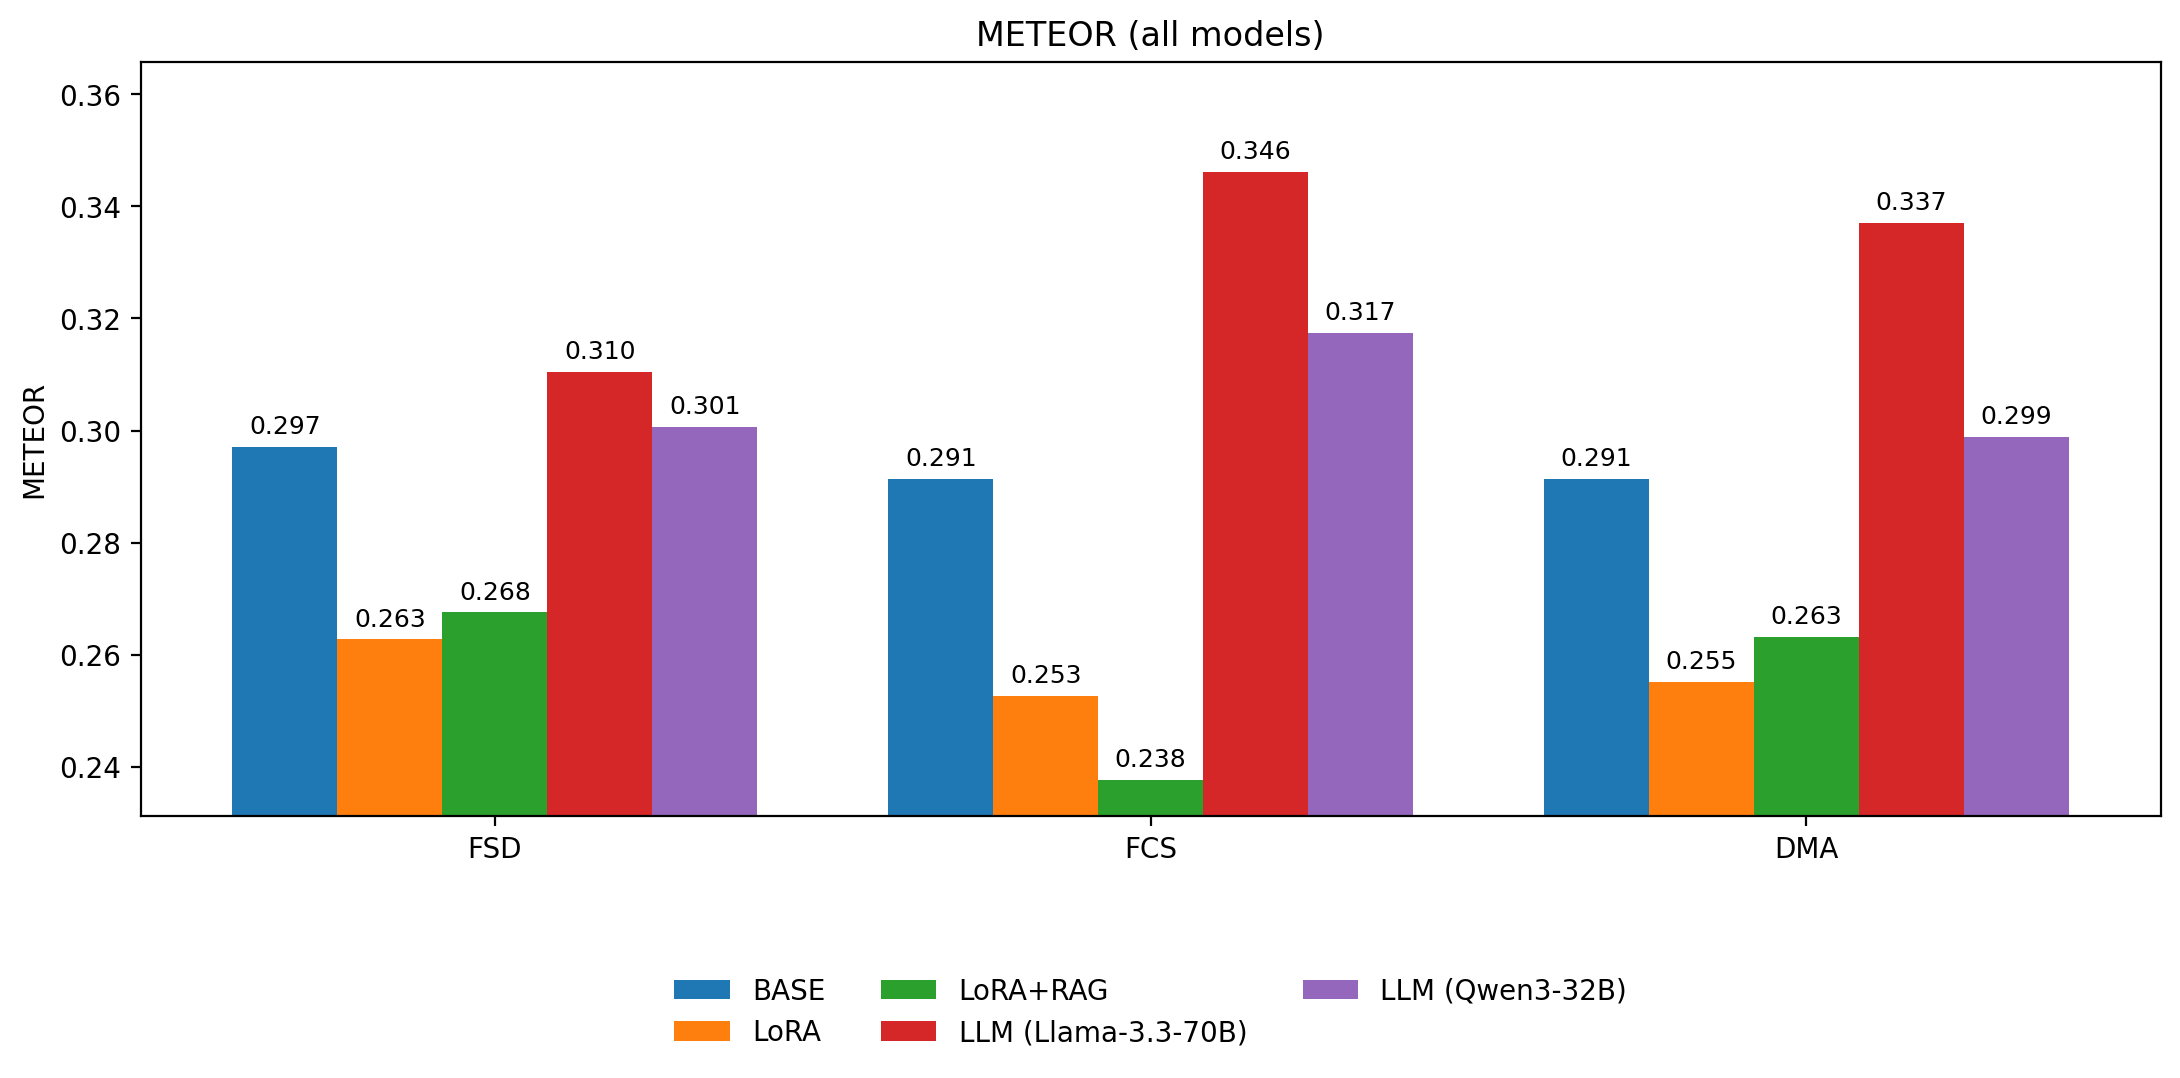
\includegraphics[width=\linewidth]{figs/all_meteor.png}
    \caption{METEOR across subjects for all models.}
    \label{fig:all-meteor}
\end{figure}
\FloatBarrier
In all three subjects, METEOR is highest for BASE and lower for LoRA / LoRA+RAG. This does not automatically mean worse tutoring quality. A likely reason is that LoRA and RAG introduce more domain-specific wording and different sentence structure, which can make unigram alignment more fragmented relative to one reference answer. At the same time, BLEU-2, ROUGE-L, and BERTScore show clear improvements, suggesting better overall alignment in wording and meaning.

\paragraph{Comparing our SLMs to LLM baselines.}
The BASE model is Phi-4-mini-instruct (approximately 3.8B parameters). We compare the subject-specific variants (BASE, LoRA, LoRA+RAG) to two larger LLM baselines (Llama-3.3-70B and Qwen3-32B).

The most important observation is that the adapted SLMs become competitive on several metrics:

\begin{itemize}
    \item \textbf{BLEU-2:} In all subjects, the best SLM (LoRA+RAG) is higher than both LLMs
    (FSD: 11.161 vs.\ Llama 8.958 vs.\ Qwen 7.761,
     FCS: 12.105 vs.\ 11.617 vs.\ 8.937,
     DMA: 10.293 vs.\ 9.805 vs.\ 7.595).
    This suggests our fine-tuning data strongly aligns the SLM outputs with the tutor reference phrasing used in the evaluation set.
    \item \textbf{BERTScore F1:} The best SLM is also higher than both LLMs in all subjects
    (FSD: 0.257 vs.\ 0.194 vs.\ 0.153,
     FCS: 0.272 vs.\ 0.243 vs.\ 0.152,
     DMA: 0.218 vs.\ 0.211 vs.\ 0.120),
    showing that subject adaptation improves meaning similarity to the reference answers.
    \item \textbf{ROUGE-L:} Llama remains slightly higher, but the gap is small in FSD
    (FSD: 0.212 vs.\ best SLM 0.209).
    In FCS and DMA the gap is larger (0.237 vs.\ 0.211, 0.211 vs.\ 0.203), while Qwen is consistently lower.
    \item \textbf{METEOR:} The LLMs score higher, especially Llama (FSD: 0.310, FCS: 0.346, DMA: 0.337),
    which is consistent with METEOR favouring closer word-level alignment and ordering relative to the single reference.
\end{itemize}

\paragraph{Latency.}
Figures \ref{fig:all-lat-mean} and \ref{fig:all-lat-median} show the runtime cost in this setup.

\begin{figure}[h]
    \centering
    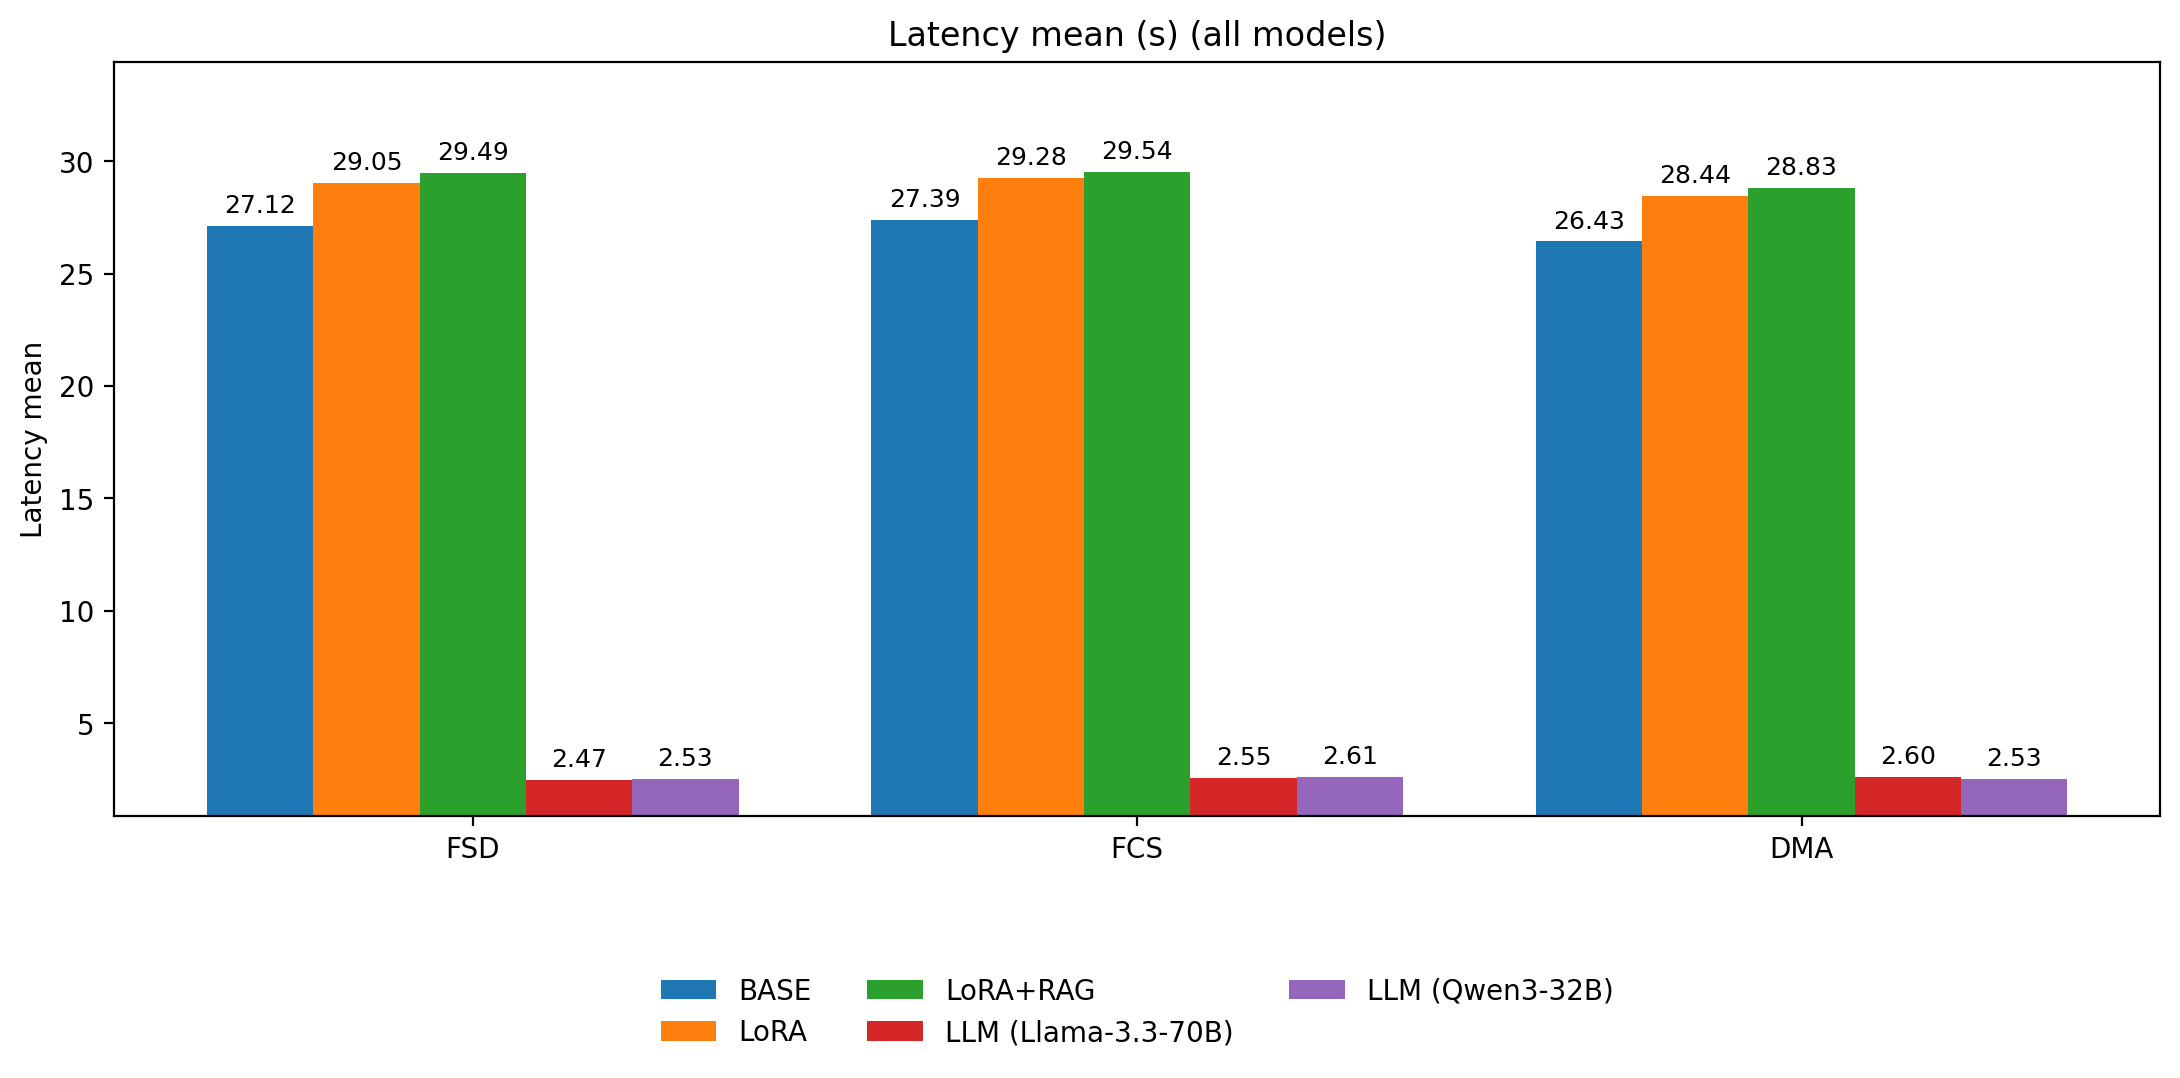
\includegraphics[width=\linewidth]{figs/all_latency_mean.png}
    \caption{Mean latency (seconds) across subjects for all models.}
    \label{fig:all-lat-mean}
\end{figure}

\begin{figure}[h]
    \centering
    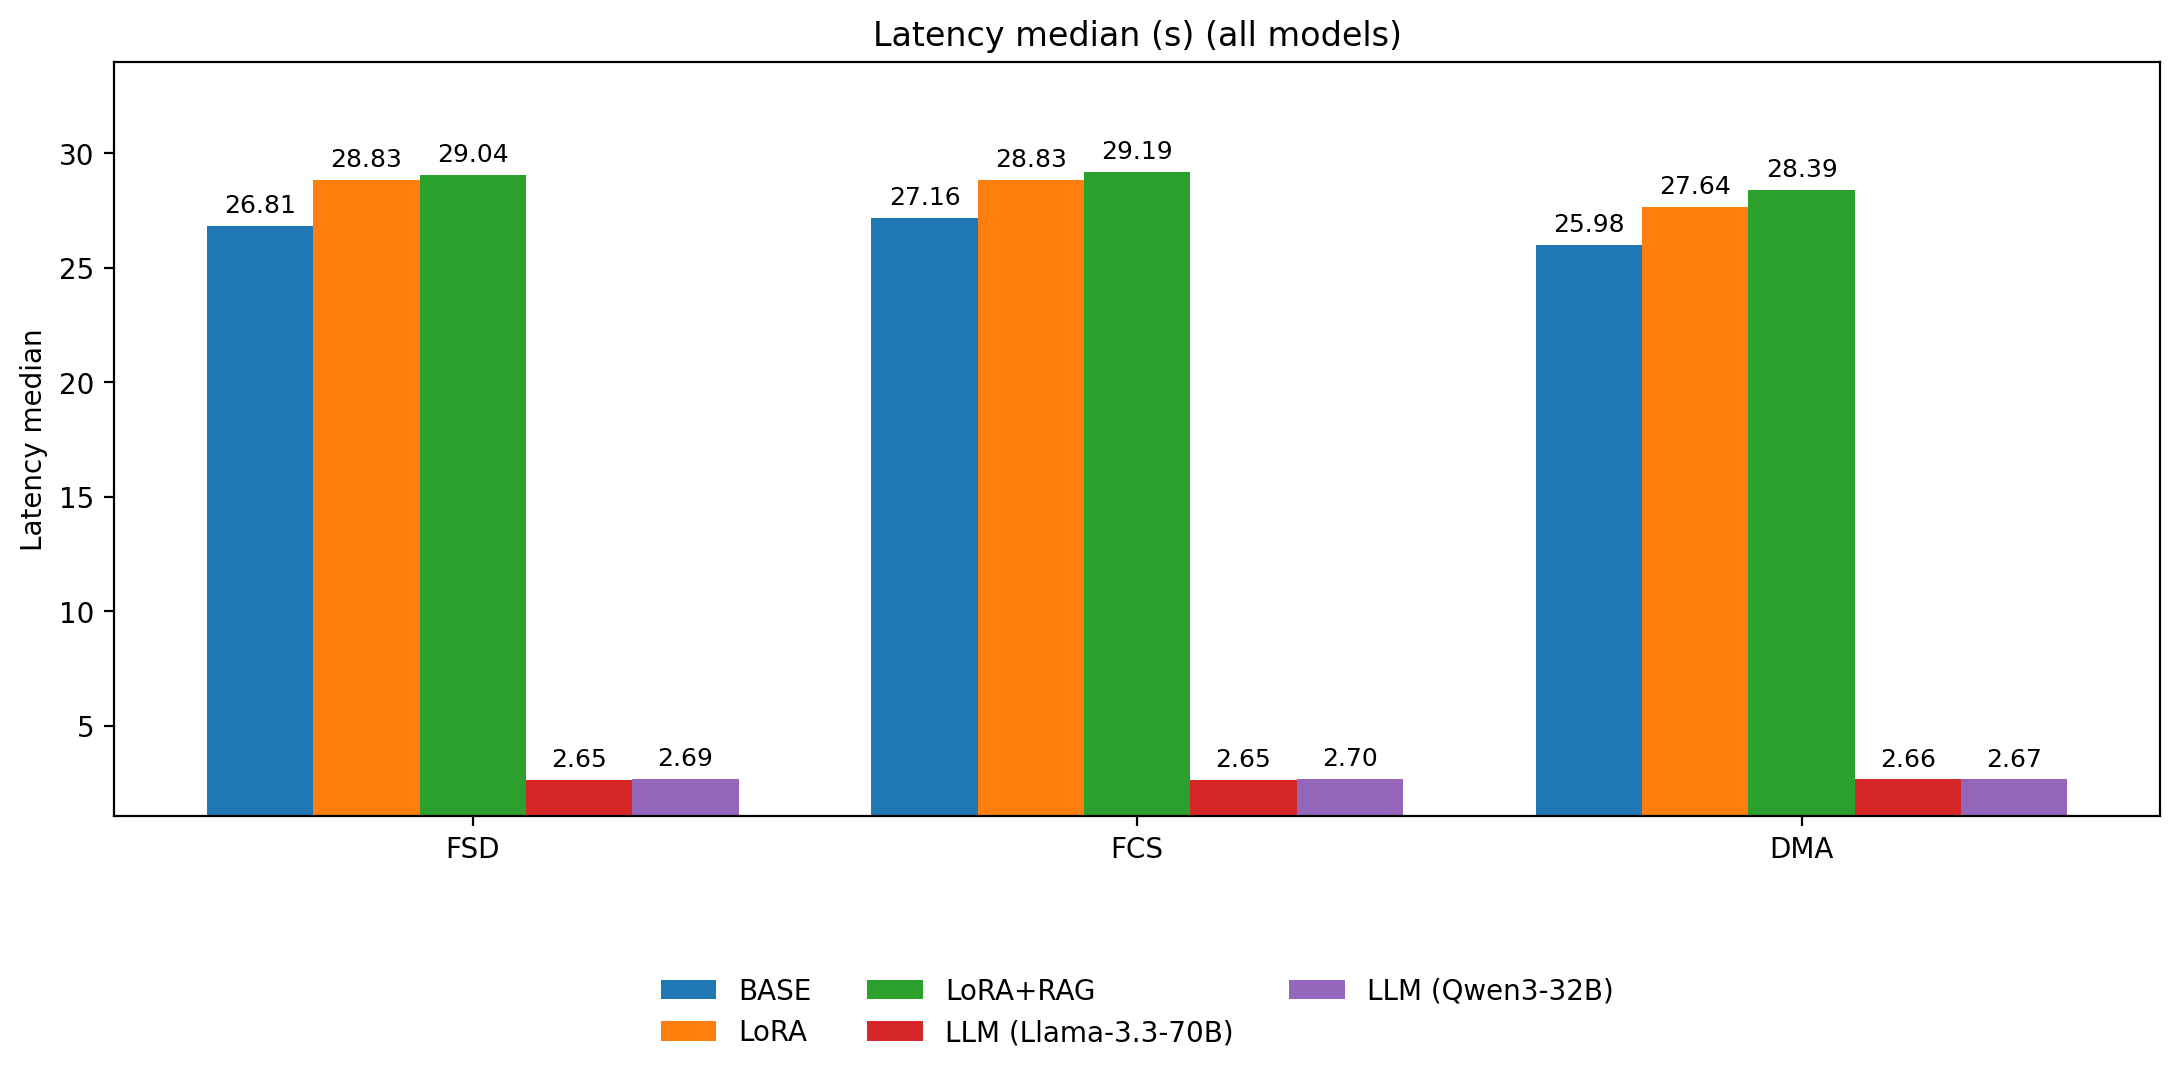
\includegraphics[width=\linewidth]{figs/all_latency_median.png}
    \caption{Median latency (seconds) across subjects for all models.}
    \label{fig:all-lat-median}
\end{figure}
\FloatBarrier
In this setup, the LLM baselines are much faster (about 2.4-2.7 seconds) than the SLM variants (about 26-30 seconds). This is likely driven by differences in serving stack and hardware configuration rather than model size alone. Within the SLM variants, LoRA+RAG is usually the slowest because retrieval increases prompt length.


\subsection{Key findings}
LoRA fine-tuning is the main reason for quality improvement across FSD, FCS, and DMA. Compared to BASE (Phi-4-mini-instruct, 3.8B parameters), LoRA consistently increases BLEU-2, ROUGE-L, and BERTScore F1. This means the SLM becomes closer to the reference tutor answers both in wording (lexical overlap) and in meaning (semantic similarity). These improvements support the project aim: small, subject-specific models can be adapted to produce more tutor-like explanations without training a large model from scratch.

RAG gives smaller and less consistent gains than LoRA. In FSD and DMA, LoRA+RAG improves BLEU-2 and ROUGE-L further, while in FCS the effect is mixed (BLEU-2 slightly increases, but ROUGE-L is almost unchanged). This is expected when evaluation uses only one reference answer: retrieval can add correct details or change phrasing, which may help tutoring quality but does not always increase overlap with a single reference.

METEOR often decreases after LoRA/RAG. A likely reason is that adapted models use more domain-specific wording and a different sentence structure, which reduces word-level alignment and increases fragmentation relative to the single reference, even when answers remain correct and clear.

When comparing to the LLM baselines (Llama-3.3-70B and Qwen3-32B), the picture depends on the metric. The best SLM variants are already competitive and in this evaluation they outperform both LLMs on BLEU-2 and BERTScore F1 in all three subjects. At the same time, Llama generally remains higher on ROUGE-L and METEOR, which suggests closer word-order alignment to the reference. Finally, latency is mainly driven by the serving setup: in this environment the LLM baselines are much faster (about 2.4-2.7 seconds), while the SLM variants take about 26-30 seconds, and RAG increases runtime due to longer prompts.

\section{Model deployment}

\section{Monitoring and maintenance}

\section{Lifecycle management}

\section{Reflection on the Progress}

